%definira klasu dokumenta 
\documentclass[12pt]{report} 

%prostor izmedu naredbi \documentclass i \begin{document} se zove uvod. U njemu se nalaze naredbe koje se odnose na cijeli dokument

%osnovni LaTex ne može riješiti sve probleme, pa se koriste različiti paketi koji olakšavaju izradu željenog dokumenta
\usepackage[croatian]{babel} 
\usepackage{amssymb}
\usepackage{amsmath}
\usepackage{txfonts}
\usepackage{mathdots}
\usepackage{titlesec}
\usepackage{array}
\usepackage{lastpage}
\usepackage{etoolbox}
\usepackage{tabularray}
\usepackage{color, colortbl}
\usepackage{adjustbox}
\usepackage{geometry}
\usepackage[classicReIm]{kpfonts}
\usepackage{hyperref}
\usepackage{fancyhdr}

\usepackage{float}
\usepackage{setspace}
\restylefloat{table}


\patchcmd{\chapter}{\thispagestyle{plain}}{\thispagestyle{fancy}}{}{} %redefiniranje stila stranice u paketu fancyhdr

%oblik naslova poglavlja
\titleformat{\chapter}{\normalfont\huge\bfseries}{\thechapter.}{20pt}{\Huge}
\titlespacing{\chapter}{0pt}{0pt}{40pt}


\linespread{1.3} %razmak između redaka

\geometry{a4paper, left=1in, top=1in,}  %oblik stranice

\hypersetup{ colorlinks, citecolor=black, filecolor=black, linkcolor=black,	urlcolor=black }   %izgled poveznice


%prored smanjen između redaka u nabrajanjima i popisima
\newenvironment{packed_enum}{
	\begin{enumerate}
		\setlength{\itemsep}{0pt}
		\setlength{\parskip}{0pt}
		\setlength{\parsep}{0pt}
	}{\end{enumerate}}

\newenvironment{packed_item}{
	\begin{itemize}
		\setlength{\itemsep}{0pt}
		\setlength{\parskip}{0pt}
		\setlength{\parsep}{0pt}
	}{\end{itemize}}




%boja za privatni i udaljeni kljuc u tablicama
\definecolor{LightBlue}{rgb}{0.9,0.9,1}
\definecolor{LightGreen}{rgb}{0.9,1,0.9}

%Promjena teksta za dugačke tablice
\DefTblrTemplate{contfoot-text}{normal}{Nastavljeno na idućoj stranici}
\SetTblrTemplate{contfoot-text}{normal}
\DefTblrTemplate{conthead-text}{normal}{(Nastavljeno)}
\SetTblrTemplate{conthead-text}{normal}
\DefTblrTemplate{middlehead,lasthead}{normal}{Nastavljeno od prethodne stranice}
\SetTblrTemplate{middlehead,lasthead}{normal}

%podesavanje zaglavlja i podnožja

\pagestyle{fancy}
\lhead{Programsko inženjerstvo}
\rhead{Program konferencije}
\lfoot{Koke}
\cfoot{stranica \thepage/\pageref{LastPage}}
\rfoot{\today}
\renewcommand{\headrulewidth}{0.2pt}
\renewcommand{\footrulewidth}{0.2pt}


\begin{document} 
	
	
	
	\begin{titlepage}
		\begin{center}
			\vspace*{\stretch{1.0}} %u kombinaciji s ostalim \vspace naredbama definira razmak između redaka teksta
			\LARGE Programsko inženjerstvo\\
			\large Ak. god. 2022./2023.\\
			
			\vspace*{\stretch{3.0}}
			
			\huge Kokeferencije\\
			\Large Dokumentacija, Rev. \textit{2.}\\
			
			\vspace*{\stretch{12.0}}
			\normalsize
			Grupa: \textit{Koke}\\
			Voditeljica: \textit{Nikoleta Benić}\\
			
			
			\vspace*{\stretch{1.0}}
			Datum predaje: \textit{13. siječnja 2023.}\\
	
			\vspace*{\stretch{4.0}}
			
			Nastavnik: \textit{Miljenko Krhen}\\
		
		\end{center}

	
	\end{titlepage}

	
	\tableofcontents


	\chapter{Dnevnik promjena dokumentacije}
				
		
		\begin{longtblr}[
				label=none
			]{
				width = \textwidth, 
				colspec={|X[2]|X[13]|X[3]|X[3]|}, 
				rowhead = 1
			}
			\hline
			\textbf{Rev.}	& \textbf{Opis promjene/dodatka} & \textbf{Autori} & \textbf{Datum}\\[3pt] \hline
			0.1 & Napravljen predložak.	& Andrea Kaselj & 31.10.2022. 		\\[3pt] \hline 
			0.2	& Zapisani dotadašnji sastanci u dodatku. & Andrea Kaselj & 31.10.2022. \\[3pt] \hline 
			0.3 & Dodana 4 Use Case i 2 sekvencijska dijagrama & Ana Ćepić & 12.11.2022.	\\[3pt] \hline 
			0.4 & Dodana 4 \textit{Use Case} dijagrama & Iva Ursić & 14.11.2022. \\[3pt] \hline 
            0.5. & Dodani opisi tablica baze podataka & Josipa Markić & 14.11.2022. \\[3pt] \hline
            0.5.1 & Dijagram baze podataka & Dorotea Dragojević & 15.11.2022. \\[3pt] \hline  
            0.5.2 & Popravljeni opisi tablica baze podataka & Josipa Markić & 16.11.2022. \\[3pt] \hline
			0.6 & Opis projektnog zadatka & Valentina Valić & 16.11.2022. \\[3pt] \hline 
			0.7 & Dodana 4 \textit{Use case} dijagrama & Nikoleta Benić & 16.11.2022. \\[3pt] \hline 
			0.8 & Dodana 4 \textit{Use case} dijagrama & Andrea Kaselj & 16.11.2022. \\[3pt] \hline 
			0.9 & Opisani nefunkcionalni zahtjevi & Andrea Kaselj & 16.11.2022. \\[3pt] \hline 
            0.9.1 & Ispravljeni \textit{Use Case} & Nikoleta Benić & 17.11.2022. \\[3pt] \hline 
			0.9.2 & Ispravljeni Use Case dijagrami & Ana Ćepić & 17.11.2022. \\[3pt] \hline
			0.9.3 & Ispravljena naslovna strana & Josipa Markić & 17.11.2022. \\[3pt] \hline
            0.9.4 & Popunjena tablica aktivnosti & Dorotea Dragojević & 17.11.2022. \\[3pt] \hline
            0.9.5 & Opisana arhitektura sustava & Andrea Kaselj & 18.11.2022. \\[3pt] \hline
		 0.9.6 & Dodan dijagram razreda & Nikoleta Benić & 18.11.2022. \\[3pt] \hline
    1.0 & Popravak i provjera dokumentacije & Nikoleta Benić & 18.11.2022. \\[3pt] \hline
    1.1 & Dodan dijagram aktivnosti za system ownera & Dorotea Dragojević & 3.1.2023. \\[3pt] \hline
    1.1.1 & Dodan dijagram aktivnosti za glavnog admina, operativnog admina i korisnika & Dorotea Dragojević & 7.1.2023. \\[3pt] \hline
     1.1.2 & Dodano ispitivanje komponenti & Dorotea Dragojević & 7.1.2023. \\[3pt] \hline
     1.1.3 & Aktivnosti grupe & Dorotea Dragojević & 7.1.2023. \\[3pt] \hline
     1.1.4 & Grafovi promjena datoteka & Dorotea Dragojević & 10.1.2023. \\[3pt] \hline
     1.2 & Ispravak tablica baze podataka & Josipa Markić & 10.1.2023. \\[3pt] \hline
    1.2.1 & Ispravljena naslovna strana & Josipa Markić & 10.1.2023. \\[3pt] \hline
    1.2.2 & Relacijski model baze & Josipa Markić & 10.1.2023. \\[3pt] \hline
	1.3 & Dodano ispitivanje komponenti & Iva Ursić & 10.1.2023. \\[3pt] \hline
	1.3.1 & Dodan zaključak & Iva Ursić & 10.1.2023. \\[3pt] \hline
	1.3.2 & Nadopunjeni nefunkcionalni zahtjevi & Iva Ursić & 10.1.2023. \\[3pt] \hline
	1.3.3 & Dodani novi sekvencijski dijagrami & Josipa Markić & 10.1.2023. \\[3pt] \hline
	1.3.4 & Dodane korištene tehnologije i alati & Valentina Valić & 10.1.2023. \\[3pt]
    \hline
    	1.3.5 & Dodana literatura & Valentina Valić & 10.1.2023. \\[3pt]
    \hline
	1.4 & Ažurirani dijagrami razreda & Nikoleta Benić & 10.1.2023. \\[3pt] \hline
	1.4.1 & Dodane upute za puštanje u pogon & Nikoleta Benić & 11.1.2023. \\[3pt] \hline
	1.5 & Dodani novi sekvencijski dijagrami & Ana Ćepić & 11.1.2023. \\[3pt]
     \hline
	1.5.1 & Uređeni obrasci uporabe & Ana Ćepić & 11.1.2023. \\[3pt]
    \hline
	1.6 & Dodani dijagram komponenti & Ana Ćepić & 11.1.2023. \\[3pt]
    \hline
	1.7 & Dodan dijagram stanja & Nikoleta Benić & 11.1.2023. \\[3pt]
    \hline
	1.8 & Dodan dijagram razmještaja & Josipa Markić & 11.1.2023. \\[3pt]
    \hline
	1.8.1 & Dodani use case dijagrami & Iva Ursić & 11.1.2023. \\[3pt]
    \hline
	1.9 & Ispravci i provjera & Josipa Markić & 11.1.2023. \\[3pt]
    \hline
	1.9.1 & Ispravak use case dijagrama & Iva Ursić & 11.1.2023. \\[3pt]
    \hline
	1.9.2 & Ispitivanje sustava & Nikoleta Benić & 12.1.2023. \\[3pt]
 \hline
	1.9.3 & Ispravak opisa projektnog zadatka & Valentina Valić & 12.1.2023. \\[3pt]
    \hline
	2.0 & Pregled dokumentacije & Iva Ursić & 13.1.2023. \\[3pt]
    \hline
		\end{longtblr}
       
	

	\chapter{Opis projektnog zadatka}
		
	
		
	
    Cilj ovog projekta je razviti programsku podršku 
    za stvaranje web aplikacije “Program Konferencije” 
    koja pruža učinkovit informacijski sustav koji omogućuje
    praćenje dolazaka sudionika na konferenciju, 
    sudjelovanje sudionika u glavnim i popratnim događanjima na
    konferenciji i davanje svih potrebnih informacija sudionicima. 
    Registriranim korisnicima konferencije informacijski 
    sustav služi kao temeljno mjesto za dobivanje informacije,
    dok organizator pomoću njega ima mogućnost distribucije 
    raznih materijala sudionicima, davanja svih potrebnih 
    informacija te praćenja aktivnosti sudionika 
    tijekom konferencije. 
    Ako korisnik nije registriran, na web stranici može 
    vidjeti samo temeljni opis događaja i tema o kojima 
    se raspravlja na konferenciji.
    \newline
    \newline
    Četiri su vrste korisnika u informacijskom sustavu:
    
    \item\textbf{Vlasnik sustava} određuje administratora za svaku pojedinu konferenciju te kreira
    generalne podatke o konferencijama čiji se rad prati.
		
	\item\textbf{Glavni administrator} konferencije imenuje operativne administratore,  te upisuje konkretne i detaljne podatke o konferenciji. Sustav mu mora omogućiti pregled prijavljenih sudionika, pregled po državama od kuda sudionici dolaze, pregled po njihovim statusima te broj prijavljenih sudionika na pojedinim posebnim događanjima. Glavni administrator ima mogućnost 
	upisa do najviše 15 grupa podataka o nekoj konferenciji, a pritom su obavezni dijelovi za svaku konferenciju:
	\begin{itemize}
		    \item   Raspored predavanja
		    \item   Prezentacije predavanja u pdf formatu dostupne svim sudionicima za preuzimanje
		    \item  Zbornik radova u pdf formatu dostupan svim sudionicima za preuzimanje
		    \item   Mjesto događanja
		\end{itemize}
		\newline
	   Također ima mogućnost postaviti sve multimedijske materijale na poslužitelj kako bi registrirani korisnici imali pristup tim materijalima u obliku pregleda te može preuzeti pdf s podacima o konferenciji.
		
		\item\textbf{Operativni administrator} koji prilikom dolaska na konferenciju svakom sudioniku dodjeljuje, tj. aktivira korisnički račun koji sudionik potom mora potvrditi putem elektroničke pošte. Za svakog korisnika treba upisati:
		\begin{itemize}
		    \item   Ime i prezime
		    \item   Broj telefona
		    \item   Adresu elektroničke pošte pod pretpostavkom da je svi sudionici koriste
		    \item   Adresu
		    \item   Državu
		    \item Naziv institucije ili poduzeća iz kojeg dolazi
		    \item Svojstvo sudjelovanja na konferenciji (gost, predavač, pozvani predavač, sudionik s objavljenim radom u zborniku, sudionik s plaćenom kotizacijom bez predavanja, pratnja sudionika)

		\end{itemize}
		
		\item\textbf{Sudionik konferencije} čija je funkcija da pregledava podatke namijenjene sudionicima. Može se registrirati tek nakon početka i dolaska na konferenciju. Kako bi registracija bila uspješna potrebno je provjeriti zadovoljava li sudionik sve zahtjeve za registracijom, a ti su podaci dostupni u drugom, tj. nezavisnom informacijskom sustavu. Registrirani sudionik može izdati zahtjev o potvrdi za sudjelovanjem u obliku pdf datoteke koja će biti izrađena na službenom dokumentu, tj. memorandumu konferencije. Na njoj će biti navedeno da je sudionik (imenom i prezimenom) sudjelovao na određenoj konferenciji u navedenom vremenskom terminu.
		\newline
		\newline
		Nakon kreiranja konferencije u sustavu upisuju se njeni podatci, a dostupni su do 30 dana nakon njenog završetka nakon čega se korisnicima zabranjuje pristup, osim glavnom administratoru koji ima period od 40 dana nakon završetka konferencije za spremanje svih podataka i zaključivanje rada s aplikacijom. Također se treba omogućiti prikaz podataka o trenutnim vremenskim uvjetima i prognozi vremena za lokaciju održavanja konferencije sudionicima što se preuzima od nekog javno dostupnog servisa. Obzirom da se sva događanja tijekom rada konferencije snimaju i slikaju od strane ovlaštenog fotografa na stranici postoji obavijest da se događaji snimaju. Potrebno je omogućiti pregled konferencija putem javno nedostupnog Youtube kanala kroz aplikaciju. Kanalu je moguće pristupiti preko poveznice koja se nalazi u aplikaciji. Pregled multimedijskih materijala napravljen je po danima, a pristupa im se zasebno za svaki pojedini dan. Po želji se pojedini materijali mogu skinuti i na lokalno računalo.
		\newline
		Tijekom konferencije su predviđena i posebna događaja te je broj mjesta na njima ograničen. Zbog toga se svaki sudionik treba prijaviti ukoliko želi na njima sudjelovati, a dozvoljeni broj sudionika je definiran od strane glavnog organizatora konferencije. Ukoliko nakon prijave sudionika sustav ustanovi da nema više slobodnih mjesta, glavnog administratora se obavještava putem elektroničke pošte o dostignutom najvećem broju sudionika na nekom događaju te ga se upućuje na potrebu rješavanja prekomjernih zahtjeva. Glavni administrator naknadno može povećati broj mogućih sudionika na nekom posebnom događaju, u tome slučaju se sudionici koji su na listi čekanja automatski prijavljuju na posebni događaj te dobivaju obavijest na mail da mogu pohađati taj posebni događaj.
		\newline
	    Sustav mora omogućiti istovremeni rad svih korisnika sustava i   
	    unos hrvatskih dijakritičkih znakova.

	\chapter{Specifikacija programske potpore}
		
	\section{Funkcionalni zahtjevi}
			
			
			\noindent \textbf{Dionici:}
			
			\begin{packed_enum}
				
				\item Vlasnik sustava
				\item Glavni administrator konferencije				
				\item Operativni administrator
				\item Sudionik konferencije
				\item Razvojni tim
				\item Baza podataka
                \item Cloudinary
                \item Poslužitelj za vremensku prognozu
				
			\end{packed_enum}
			
			\noindent \textbf{Aktori i njihovi funkcionalni zahtjevi:}
			
			
			\begin{packed_enum}
				\item  \underbar{Neprijavljeni korisnik može:}
				
				\begin{packed_enum}
					
					\item pregledati aktivne konferencije i temeljne podatka o svakoj od tih konferencija
					
				\end{packed_enum}
			
				\item  \underbar{Vlasnik sustava može:}
				
				\begin{packed_enum}
    
                        \item Prijaviti se u sustav					
					\item Dodati konferenciju
					\item Kreirati korisnički račun glavnog admina svake konferencije
					
				\end{packed_enum}
				
				\item  \underbar{Glavni administrator može:}
				
				\begin{packed_enum}

                        \item Prijaviti se u sustav	
					\item Unijeti grupe podataka za konferenciju
					\item Kreirati korisničke račune za operativne admine konferencije
					\item Spremiti podatke o konferenciji nakon njenog završetka u obliku PDFa
					\item Postaviti multimedijske materijale sa konferencije i skinuti ih
					\item Pregledati sudionike konferencije po ulozi i državi iz koje dolaze
                        \item Kreirati poseban događaj i po potrebi povećati kapacitet
                        \item Pregledati detaljne podatke o svojoj konferenciji
					
				\end{packed_enum}
				
				\item  \underbar{Operativni administrator može:}
				
				\begin{packed_enum}

                         \item Prijaviti se u sustav	
					\item Kreirati korisničke račune sudionika konferencije
                        \item Pregledati detaljne podatke o svojoj konferenciji
					
				\end{packed_enum}
				
				\item  \underbar{Sudionik konferencije može:}
				
				\begin{packed_enum}

                        
					\item Prijaviti se u sustav
					\item Pregledati multimedijske materijale i skinuti ih
					\item Prijaviti se na posebna događanja
					\item Skinuti PDF potvrdu o sudjelovanju
                        \item Pregledati detaljne podatke o svojoj konferenciji
					
				\end{packed_enum}
				
				\item  \underbar{Baza podataka može:}
				
				\begin{packed_enum}
					
					\item Pohranjivati podatke o konferencijama
					\item Pohranjivati podatke o registriranim korisnicima
                        \item Pohranjivati podatke o posebnim događajima
                        \item Pohranjivati podatke o multimediji
                        \item Pohranjivati podatke o grupama podataka
					
				\end{packed_enum}
			\end{packed_enum}
			
			\eject 
			
			
				
			\subsection{Obrasci uporabe}
				
				
				\subsubsection{Opis obrazaca uporabe}
			
									\noindent \underbar{\textbf{UC1 -Pregled aktivnih konferencija}}
					\begin{packed_item}

                            
						\item \textbf{Glavni sudionik: }neprijavljeni korisnik, prijavljeni korisnik(sudionik, glavni admin, vlasnik sustava, operativni admin)
						\item  \textbf{Cilj:} Pregledati aktivne konferencije
						\item  \textbf{Sudionici:} Baza podataka
						\item  \textbf{Preduvjet:} -
						\item  \textbf{Opis osnovnog tijeka:}
						
						\item[] \begin{packed_enum}
	
							\item Popis konferencija vidljiv je odmah nakon pokretanja aplikacije
							\item Prikazuju se osnovne informacije o konferenciji: grad održavanja, opis konferencije i teme
						\end{packed_enum}
					\end{packed_item}

     \noindent \underbar{\textbf{UC2 - Registracija glavnog admina}}
					\begin{packed_item}
	
						\item \textbf{Glavni sudionik: }vlasnik sustava
						\item  \textbf{Cilj:} Stvoriti korisnički račun za  glavnog admina konferencije
						\item  \textbf{Sudionici:} Baza podatka, glavni admin
						\item  \textbf{Preduvjet:} -
						\item  \textbf{Opis osnovnog tijeka:}
						
						\item[] \begin{packed_enum}

							\item Vlasnik sustava odabere opciju \textit{Registriraj}
							\item Vlasnik sustava unosi potrebne podatke: ime, prezime, broj telefona, e-mail, adresu, državu, naziv poduzeća iz koje dolazi, svojstvo sudjelovanja na konferenciji
                                \item Povratak na meni
						
						\end{packed_enum}
						\item  \textbf{Opis mogućih odstupanja:}
						
						\item[] \begin{packed_item}

                                    \item[1.]  Unos već zauzetog korisničkog imena, unos podataka u nedozvoljenom       formatu ili pružanje neispravnog e-maila:
							\item[] \begin{packed_enum}
								
								\item Sustav obavještava glavnog sudionika o neuspjelom upisu
								\item Glavni sudionik mijenja potrebne podatke te završava unos ili odustaje od registracije
							
						\end{packed_enum}
					\end{packed_item}
     \end{packed_item}

     				 \noindent \underbar{\textbf{UC3 - Registracija operativnog admina}}
					\begin{packed_item}
	
						\item \textbf{Glavni sudionik: }glavni admin
						\item  \textbf{Cilj:} Stvoriti korisnički račun za  operativnog admina konferencije
						\item  \textbf{Sudionici:} Baza podatka, operativni admin
						\item  \textbf{Preduvjet:} -
						\item  \textbf{Opis osnovnog tijeka:}
						
						\item[] \begin{packed_enum}

							\item Glavni admin odabere opciju \textit{Registriraj}
							\item Glavni admin unosi potrebne podatke: ime, prezime, broj telefona, e-mail, adresu, državu, naziv poduzeća iz koje dolazi, svojstvo sudjelovanja na konferenciji
                                \item Povratak na meni
						
						\end{packed_enum}
						\item  \textbf{Opis mogućih odstupanja:}
						
						\item[] \begin{packed_item}

                                    \item[1.]  Unos već zauzetog korisničkog imena, unos podataka u nedozvoljenom       formatu ili pružanje neispravnog e-maila:
							\item[] \begin{packed_enum}
								
								\item Sustav obavještava glavnog sudionika o neuspjelom upisu
								\item Glavni sudionik mijenja potrebne podatke te završava unos ili odustaje od registracije
							
						\end{packed_enum}
					\end{packed_item}
     \end{packed_item}

      \noindent \underbar{\textbf{UC4 - Registracija sudionika}}
					\begin{packed_item}
	
						\item \textbf{Glavni sudionik: }operativni admin
						\item  \textbf{Cilj:} Stvoriti korisnički račun za  sudionika konferencije
						\item  \textbf{Sudionici:} Baza podatka, operativni admin
						\item  \textbf{Preduvjet:} Plaćena kotizacija
						\item  \textbf{Opis osnovnog tijeka:}
						
						\item[] \begin{packed_enum}

							\item Operativni admin odabere opciju \textit{Registriraj}
							\item Operativni admin unosi potrebne podatke: ime, prezime, broj telefona, e-mail, adresu, državu, naziv poduzeća iz koje dolazi, svojstvo sudjelovanja na konferenciji
                                \item Sustav šalje mail s linkom za potvrdu registracije sudioniku
                                \item Povratak na meni
						
						\end{packed_enum}
						\item  \textbf{Opis mogućih odstupanja:}
						
						\item[] \begin{packed_item}

                                \item[1.]  Sudionik nije platio kotizaciju
							\item[] \begin{packed_enum}
								
								\item Odustaje se od registracije

                                    \item[2.]  Unos već zauzetog korisničkog imena, unos podataka u nedozvoljenom       formatu ili pružanje neispravnog e-maila:
							\item[] \begin{packed_enum}
								
								\item Sustav obavještava glavnog sudionika o neuspjelom upisu
								\item Glavni sudionik mijenja potrebne podatke te završava unos ili odustaje od registracije
							
						\end{packed_enum}
                    \end{packed_enum}
					\end{packed_item}
     \end{packed_item}

     \noindent \underbar{\textbf{UC5 - Prijava u sustav}}
					\begin{packed_item}
	
						\item \textbf{Glavni sudionik: } Korisnik
						\item  \textbf{Cilj:} Dobiti pristup korisničkom sučelju
						\item  \textbf{Sudionici:} Baza podataka
						\item  \textbf{Preduvjet:} Registracija uspješna
						\item  \textbf{Opis osnovnog tijeka:}
						
						\item[] \begin{packed_enum}
	
							\item Korisnik odabere opciju \textit{Prijavi se}
							\item Korisnik unosi korisničko ime i lozinku
							\item Pristup korisničkim funkcijama
						\end{packed_enum}
						
						\item  \textbf{Opis mogućih odstupanja:}
						
						\item[] \begin{packed_item}
	
							\item[1.] Neispravno korisničko ime i lozinka

							\item[] \begin{packed_enum}
								
								\item Sustav obavještava korisnika o neuspjeloj prijavi porukom "Login failed"
								
							\end{packed_enum}
							
						\end{packed_item}
					\end{packed_item}

     \noindent \underbar{\textbf{UC6 - Stvaranje konferencije}}
					\begin{packed_item}
	
						\item \textbf{Glavni sudionik: } vlasnik sustava
						\item  \textbf{Cilj:} Unijeti temeljne podatke o konferenciji u sustav
						\item  \textbf{Sudionici:} Baza podataka
						\item  \textbf{Preduvjet:} -
						\item  \textbf{Opis osnovnog tijeka:}
						
						\item[] \begin{packed_enum}
	
							\item Vlasnik sustava odabere opciju \textit{Dodaj konferenciju}
							\item Vlasnik unosi temeljne podatke: naziv, mjesto i vrijeme, teme, događaji, glavnog administratora konferencije
							\item Konferencija se prikazuje u sustavu
						\end{packed_enum}

                        \item  \textbf{Opis mogućih odstupanja:}
						
						\item[] \begin{packed_item}
	
							\item[1.] Nisu uneseni svi podatci

							\item[] \begin{packed_enum}
								
								\item Sustav obavještava korisnika da mora unijeti sve podatke za konferenciju
								
							\end{packed_enum}
							
						\end{packed_item}
						
					\end{packed_item}


     					\noindent \underbar{\textbf{UC7 - Unos grupa podataka za konferenciju}}
					\begin{packed_item}
	
						\item \textbf{Glavni sudionik: } glavni administrator
						\item  \textbf{Cilj:} unijeti grupe podataka za konferenciju
						\item  \textbf{Sudionici:} baza podataka
						\item  \textbf{Preduvjet:} konferencija stvorena
						\item  \textbf{Opis osnovnog tijeka:}
						
						\item[] \begin{packed_enum}

                                \item Glavni admin najprije unosi glavne grupe podataka
							\item Glavni admin odabere opciju \textit{Unos podataka}
							\item Glavni admin unosi do najviše 15 grupa podataka među kojima su obavezni: raspored predavanja, zbornik radova, prezentacije predavanja i mjesto događaja
							\item Detaljni podaci dostupni registriranim korisnicima na pregled
						\end{packed_enum}
						
						\item  \textbf{Opis mogućih odstupanja:}
						
						\item[] \begin{packed_item}
	
							\item[1.] Nepotpuno ispunjavanje obveznih grupa podataka
							\item[] \begin{packed_enum}
								
								\item Admin ne može unijeti ostale grupe podataka

                                    \end{packed_enum}
                                \item[2.] Nepotpuno ispunjavanje forme za kreiranje neobavezne grupe podataka
							\item[] \begin{packed_enum}
								
								\item Sustav obaviještava admina da mora unijeti sve podatke
                                \end{packed_enum}
        
                                \item[3.] Admin pokušava unijeti više od 15 grupa podataka
							\item[] \begin{packed_enum}
								
								\item Sustav obaviještava admina da ne može unijeti sve podatke

                                    \end{packed_enum}
							
						\end{packed_item}
					\end{packed_item}

     \noindent \underbar{\textbf{UC8 - Spremanje podataka o konferenciji u obliku PDF-a}}
					\begin{packed_item}
	
						\item \textbf{Glavni sudionik: }Glavni administrator

						\item  \textbf{Cilj:} spremiti sve podatke prije zaključenja rada s aplikacijom
						\item  \textbf{Sudionici:} baza podataka
						\item  \textbf{Preduvjet:} -
						\item  \textbf{Opis osnovnog tijeka:}
						
						\item[] \begin{packed_enum}
	
							\item Glavni admin odabire opciju \textit{Spremi konferenciju}
							\item Podaci se spremaju na lokalno računalo u obliku PDF-a
							
						\end{packed_enum}
						
						
						\end{packed_item}

     \noindent \underbar{\textbf{UC9 - Postavljanje multimedijskih sadržaja}}
					\begin{packed_item}
	
						\item \textbf{Glavni sudionik: }Glavni administrator

						\item  \textbf{Cilj:} ponuditi pregled i skidanje multimedijskog sadržaja registriranim korisnicima
						\item  \textbf{Sudionici:} poslužitelj Cloudinary
						\item  \textbf{Preduvjet:} -
						\item  \textbf{Opis osnovnog tijeka:}
						
						\item[] \begin{packed_enum}
	
							\item Glavni admin odabire opciju \textit{Dodaj multimedijski sadržaj}
							\item Glavni admin dodaje direktorij za pojedini dan ili odabire postojeći direktorij
                                \item Glavni admin postavlja multimedijski sadržaj za pojedini dan
							
						\end{packed_enum}
                     \item  \textbf{Opis mogućih odstupanja:}
						
						\item[] \begin{packed_item}
	
							\item[1.] Pokušava se kreirati direktorij s datumom koji nije unutar datuma održavanja konferencije

							\item[] \begin{packed_enum}
								
								\item Sustav obavještava korisnika da uneseni datum nije dobar
								
							\end{packed_enum}
							
						\end{packed_item}
										
						\end{packed_item}

     \noindent \underbar{\textbf{UC10 - Pregled sudionika konferencije}}
					\begin{packed_item}
	
						\item \textbf{Glavni sudionik: }Glavni administrator

						\item  \textbf{Cilj:} Pregled prijavljenih sudionika
						\item  \textbf{Sudionici:} Baza podataka
						\item  \textbf{Preduvjet:} -
						\item  \textbf{Opis osnovnog tijeka:}
						
						\item[] \begin{packed_enum}
	
							\item Glavni admin odabere opciju \textit {Pregled prijavljenih sudionika}
							\item Prikazuju se podaci o prijavljenim sudionicima (status i država iz koje dolaze)
							
						\end{packed_enum}
						
						
						\end{packed_item}
				
						\noindent \underbar{\textbf{UC11 - Pregled multimedijskih sadržaja}}
					\begin{packed_item}
						
						\item \textbf{Glavni sudionik:} Korisnik(sudionik, glavni admin ili operativni admin)
						\item  \textbf{Cilj:} Pregled multimedijskih materijala po danima i mogućnost preuzimanja na lokalno računalo
						\item  \textbf{Sudionici:} Poslužitelj Cloudinary
						\item  \textbf{Preduvjet:} Glavni administrator konferencije je postavio multimedijske materijale na poslužitelj
						\item  \textbf{Opis osnovnog tijeka:}
						
						\item[] \begin{packed_enum}
							
							\item Korisnik odabere opciju \textit{Pregled multimedijskog sadržaja}
							\item Korisniku se prikazuju multimedijski materijali po danima
							\item Korisnik ih može preuzeti klikom na gumb "Preuzmi"
						\end{packed_enum}
					\end{packed_item}

			
						\noindent \underbar{\textbf{UC12 - Prijava na poseban događaj}}
					\begin{packed_item}
						
						\item \textbf{Glavni sudionik:} Sudionik konferencije
						\item  \textbf{Cilj:} Prijava na posebni događaj
						\item  \textbf{Sudionici:} Baza podataka
						\item  \textbf{Preduvjet:} -
						\item  \textbf{Opis osnovnog tijeka:}
						
						\item[] \begin{packed_enum}
							
							\item Korisnik odabere opciju \textit{Prijavi se na posebni događaj}
							\item Sustav ispisuje potvrdu o uspješnoj prijavi
						\end{packed_enum}
						\item  \textbf{Opis mogućih odstupanja:}
					
					\item[] \begin{packed_item}
						
						\item[1.] Sva mjesta za željeni događaj su zauzeta
						\item[] \begin{packed_enum}

                                \item Sudionik se stavlja u listu čekanja za događaj
							\item Sustav obavještava glavnog administratora o prekobrojnoj potražnji za već popunjeni događaj i mogućnosti povećanja broja sudionika
							
						\end{packed_enum}
						
					\end{packed_item}
				\end{packed_item}
			
				\noindent \underbar{\textbf{UC13 - Generiranje PDF potvrde o sudjelovanju}}
			\begin{packed_item}
				
				\item \textbf{Glavni sudionik:} Korisnik
				\item  \textbf{Cilj:} Generiranje PDF potvrde
				\item  \textbf{Sudionici:} baza podataka
				\item  \textbf{Preduvjet:} -
				\item  \textbf{Opis osnovnog tijeka:}
				
				\item[] \begin{packed_enum}
					
					\item Korisnik bira opciju \textit{Potvrda o sudjelovanju}
					\item Sustav generira PDF dokument o sudjelovanju
					\item Korisnik može preuzeti pdf potvrdu
				\end{packed_enum}
			\end{packed_item}

        \noindent \underbar{\textbf{UC14 - Povećanje kapaciteta posebnog događaja}}
			\begin{packed_item}
				
				\item \textbf{Glavni sudionik:} Glavni admin
				\item  \textbf{Cilj:} Povećanje kapaciteta posebnog događaja
				\item  \textbf{Sudionici:} baza podataka
				\item  \textbf{Preduvjet:} Popunjenost kapaciteta posebnog događaja, postoji poseban događaj
				\item  \textbf{Opis osnovnog tijeka:}
				
				\item[] \begin{packed_enum}
					
					\item Glavni admin bira opciju \textit{Povećaj kapacitet}
					\item Sustav ažurira broj mjesta na posebnom događaju
					\item Sudionik koji je bio u listi čekanja dobiva mail obavijest da se mjesto otvorilo
				\end{packed_enum}
			\end{packed_item}

    \noindent \underbar{\textbf{UC15 - Stvaranje posebnog događaja}}
			\begin{packed_item}
				
				\item \textbf{Glavni sudionik:} Glavni admin
				\item  \textbf{Cilj:} Stvoriti poseban događaj na konferenciji
				\item  \textbf{Sudionici:} baza podataka
				\item  \textbf{Preduvjet:} -
				\item  \textbf{Opis osnovnog tijeka:}
				
				\item[] \begin{packed_enum}
					
					\item Glavni admin bira opciju \textit{Kreiraj posebni događaj}
					\item Glavni admin unosi kapacitet, tip posebnog događaja i poruku sudionicima
					\item Poseban događaj se dodaje kao grupa podataka konferencije
				\end{packed_enum}
         \item  \textbf{Opis mogućih odstupanja:}
					
					\item[] \begin{packed_item}
						
						\item[1.] Nisu uneseni svi podatci
						\item[] \begin{packed_enum}

                                \item Sustav obaviještava korisnika da mora unijeti sve podatke
							
						\end{packed_enum}
						
					\end{packed_item}
			\end{packed_item}



   \noindent \underbar{\textbf{UC16 - Pregled podataka o konferenciji}}
			\begin{packed_item}
				
				\item \textbf{Glavni sudionik:} Registrirani korisnik
				\item  \textbf{Cilj:} Pregledati detaljne podatke o konferenciji
				\item  \textbf{Sudionici:} baza podataka, poslužitelj za vremensku prognozu
				\item  \textbf{Preduvjet:} -
				\item  \textbf{Opis osnovnog tijeka:}
				
				\item[] \begin{packed_enum}
					
					\item Korisnik bira opciju \textit{ Moja konferencija }
					\item Prikazuje se stranica sa svim podacima o konferenciji
         
					\end{packed_item}
			\end{packed_item}
	
     
					
				\subsubsection{Dijagrami obrazaca uporabe}
					
						\begin{figure}[H]
			            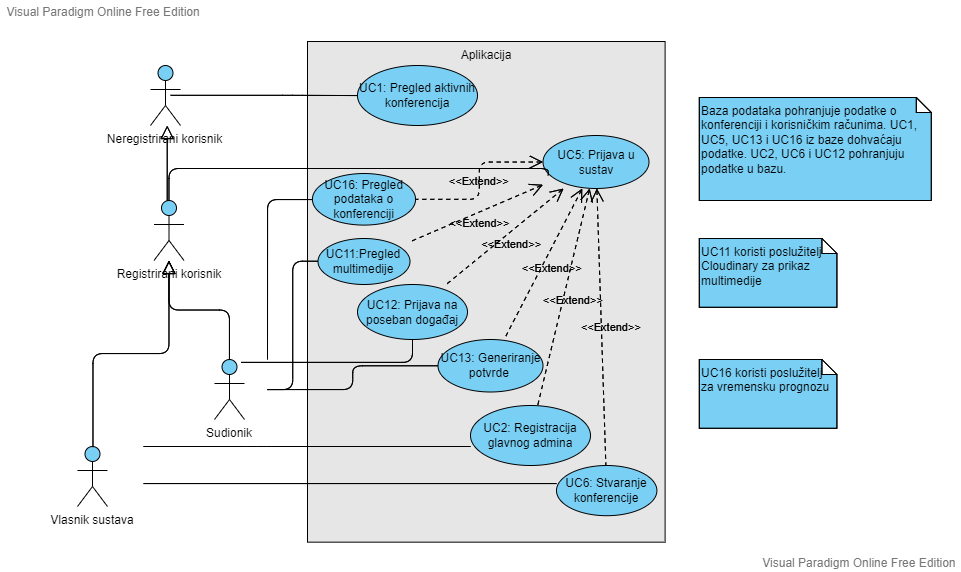
\includegraphics[scale=0.5]{slike/UC_diagram_1.png} %veličina slike u odnosu na originalnu datoteku i pozicija slike
			            \centering
			            \caption{Funkcionalnosti za sudionika i vlasnika sustava}
			            \label{fig:uc-dijagram1}
		                \end{figure}
		                
		                \begin{figure}[H]
			            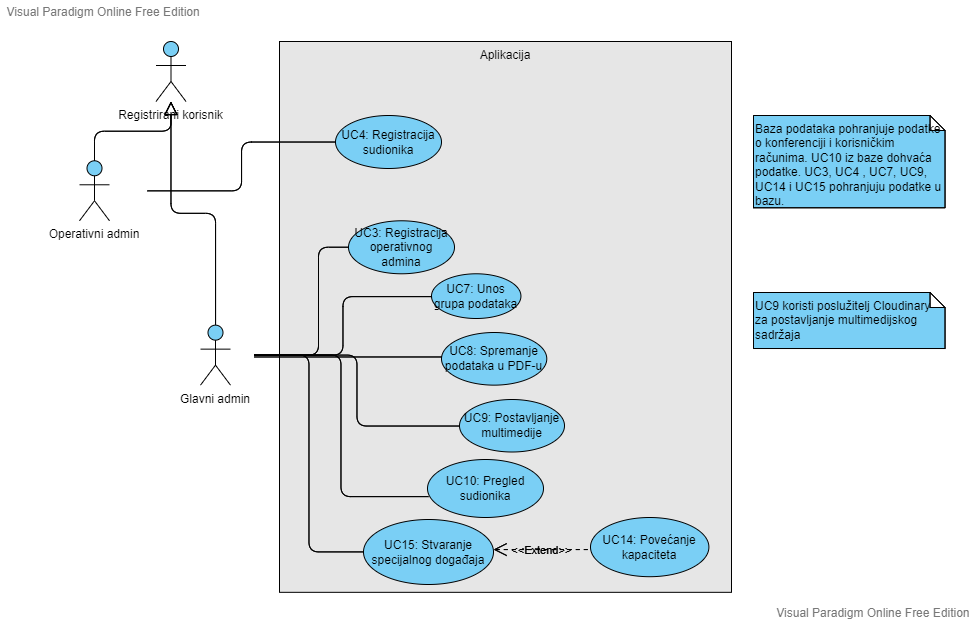
\includegraphics[scale=0.5]{slike/UC_diagram_2.png} %veličina slike u odnosu na originalnu datoteku i pozicija slike
			            \centering
			            \caption{Funkcionalnosti za glavnog admina i operativnog admina}
			            \label{fig:uc-dijagram2}
		                \end{figure}
				\eject		
				
			\subsection{Sekvencijski dijagrami}
				
	

            \textbf{UC7: Unos grupa podataka za konferenciju}\\
				
				{Glavni admin konferencije unosi grupe podataka za svoju konferenciju. Postoje 4 obavezne grupe podataka: raspored predavanja, zbornik radova, prezentacije predavanja i lokacija događanja te jedna grupa podataka koja je obavezna samo ako postoji posebni događaj - obavijest o posebnom događaju. Glavni admin mora prvo unijeti obavezne grupe podataka, a onda tek smije unijeti dodatne podatke. Moguće je unijeti maksimalno 15 grupa podataka za neku konferenciju. Ukoliko je već uneseno 15 grupa podataka aplikacija obaviještava admina porukom.}
				
		        \begin{figure}[H]
			            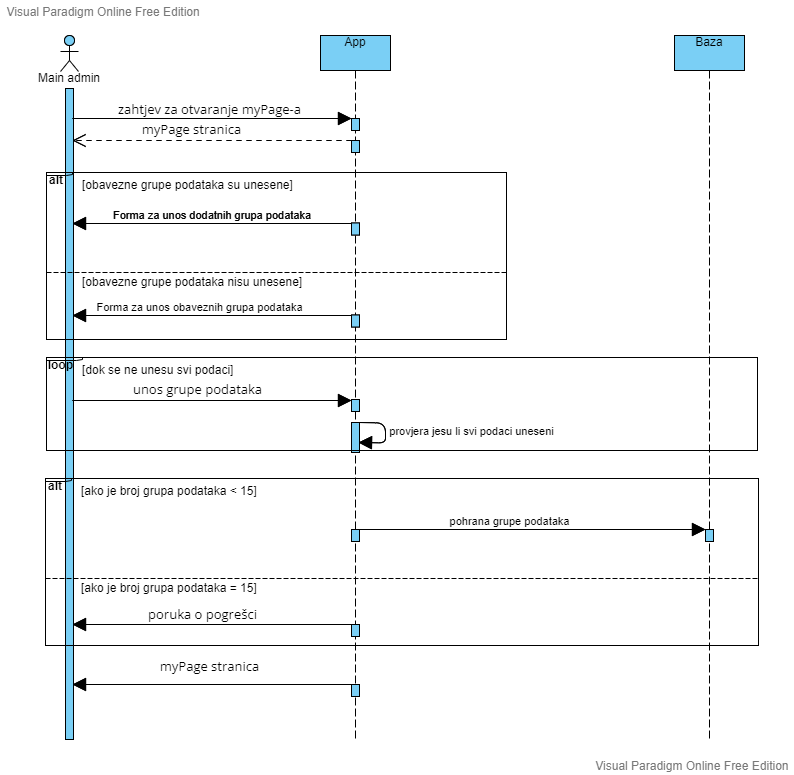
\includegraphics[scale=0.55]{slike/stvaranje grupe podataka (1).png} %veličina slike u odnosu na originalnu datoteku i pozicija slike
			            \centering
			            \caption{Unos grupe podataka}
			            \label{fig:seq-dijagram2}
		        \end{figure}\\
				
				\eject

             \textbf{UC15: Stvaranje posebnog događaja}\\
				
				{Glavni admin stvara posebna događanja za konferenciju. S obzirom da se stvaranjem posebnog događaja stvara i grupa podataka tj. obavijest, provjerava se je li dosegnut maksimalan broj grupa podataka. Ukoliko nije, stvara se posebni događaj i obavijest o tom posebnom događaju, u suprotnom se obaviještava admina o pogrešci.}
				
		        \begin{figure}[H]
			            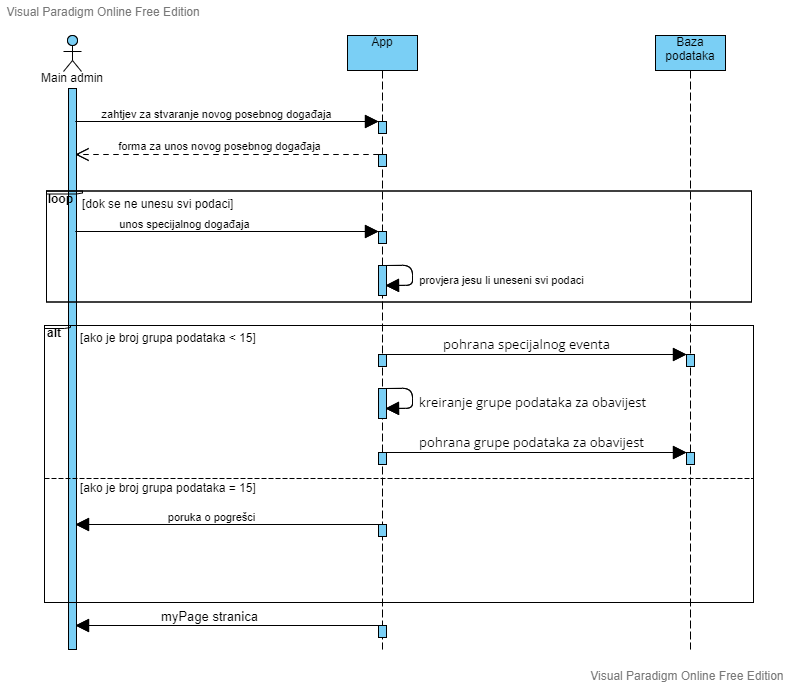
\includegraphics[scale=0.55]{slike/stvaranje spec eventa.png} %veličina slike u odnosu na originalnu datoteku i pozicija slike
			            \centering
			            \caption{Unos posebnog događaja}
			            \label{fig:seq-dijagram2}
		        \end{figure}\\
				
				\eject

             \textbf{UC5: Prijava u sustav, UC6: Stvaranje konferencije, UC2: Registracija glavnog admina}\\
				
				{Vlasnik sustava se prijavljuje u aplikaciju. Ako je prijava uspješna, vlasnik sustava dobiva pristup aplikaciji, inače dobiva poruku o neuspjeloj prijavi i može pokušati opet. Vlasnik sustava odabire opciju kreiranja konferencije i unosi glavne podatke o konferenciji. Ako nisu uneseni svi podatci, sustav to dojavljuje vlasniku. Ako je sve ispravno uneseno, stvara se nova konferencija i vlasnik sustava je preusmjeren na formu za registraciju glavnog admina te konferencije. Unosi podatke o glavnom adminu i pridružuje ga upravo napravljenoj konferenciji. Ako je sve ispravno uneseno, stvoren je račun glavnog admina i vlasnik sustava je preusmjeren na menu page, inače dobiva poruku o netočno unesenim podatcima.}
				
		        \begin{figure}[H]
			            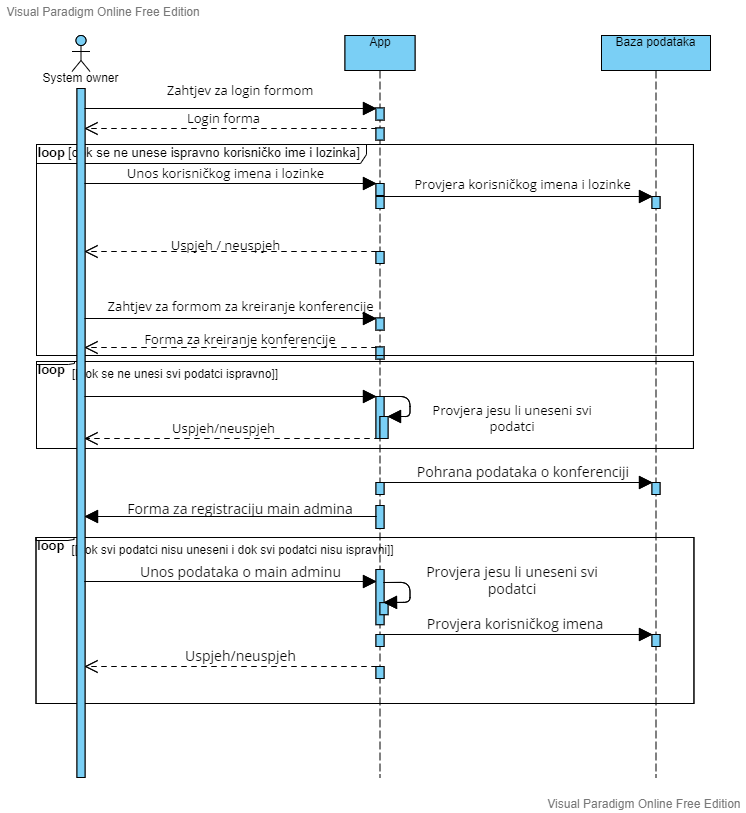
\includegraphics[scale=0.55]{slike/Stvaranje_konf_seq.png} %veličina slike u odnosu na originalnu datoteku i pozicija slike
			            \centering
			            \caption{Stvaranje konferencije i main admina konferencije}
			            \label{fig:seq-dijagram2}
		        \end{figure}\\
				
				\eject

             \textbf{UC12: Prijava na poseban događaj}\\
				
				{Sudionik konferencije odabire opciju prijave na poseban događaj. Ako ima još slobodnih mjesta, korisnik postaje sudionik tog posebnog događaja, a broj slobodnih mjesta se umanjuje za jedan. Ako nema slobodnih mjesta, sudionik se stavlja u listu čekanja, a sustav šalje mail obavijest glavnom adminu konferencije da su sva mjesta na specijalnom događaju popunjena. Nakon toga, glavni admin može povećati broj mjesta. Ako to učini, sustav šalje mail obavijest korisniku da je primljen na poseban događaj te ažurira broj slobodnih mjesta.}
				
		        \begin{figure}[H]
			            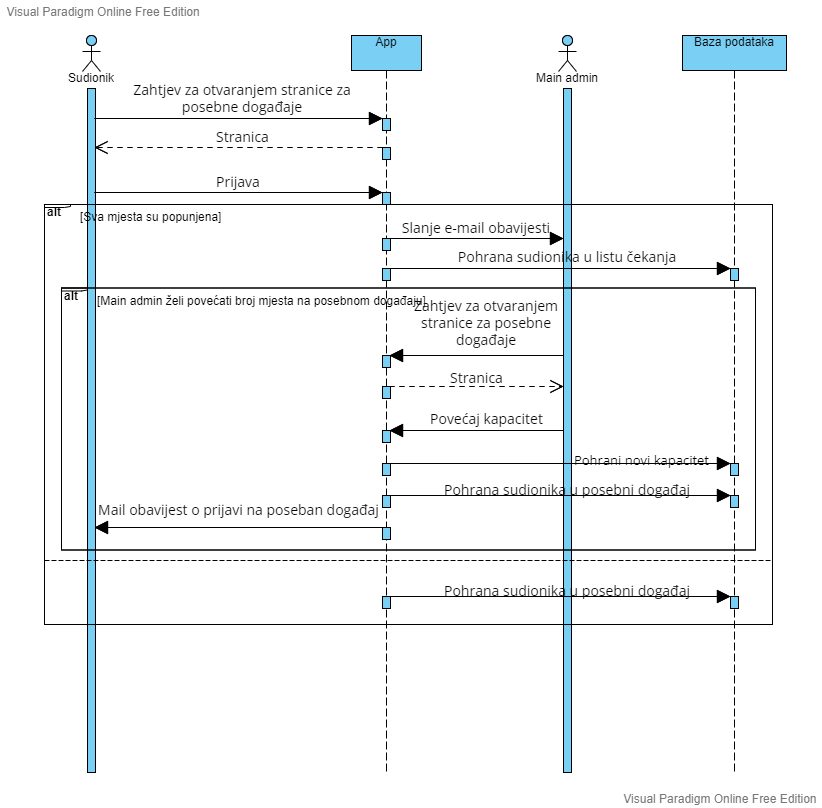
\includegraphics[scale=0.55]{slike/Spec_event_prijava_seq.png} %veličina slike u odnosu na originalnu datoteku i pozicija slike
			            \centering
			            \caption{Prijava na poseban događaj}
			            \label{fig:seq-dijagram2}
		        \end{figure}\\
	
				\eject
	
		\section{Nefunkcionalni zahtjevi}
		
		 
			\begin{packed_item}  
				 \item Sustav treba biti implementiran kao web aplikacija koristeći objektno-orijentirane jezike
				 \item Pristup sustavu mora biti omogućen iz javne mreže pomoću HTTPS
				 \item Sustav treba omogućiti rad više korisnika u stvarnom vremenu, preko 500
				 \item Sustav treba biti izdržljiv na neispravno korištenje
				 \item Izvršavanje dijela programa u kojem se pristupa bazi podataka ne smije trajati duže od nekoliko sekundi
				 \item Nadogradnja sustava ne smije narušavati postojeće funkcionalnosti sustava
				 \item Veza s bazom podataka mora biti zaštićena i otporna na vanjske greške
				 \item Učitavanje prikaza ne smije trajati duže od nekoliko sekundi
				 \item Pristup sustavu treba biti omogućen samo registriranim korisnicima i zaštićen od vanjskih sudionika
                \item Tokeni za potvrdu e-mail adrese traju 24 sata
                \item Tokeni za autentifikaciju traju 1 sat
                \item Korisničko sučelje i sustav moraju podržavati hrvatsku abecedu (dijakritičke znakove) pri unosu i prikažu tekstualnog sadrzaja
                \item Neispravno korištenje korisničkog sučelja ne smije narušiti funkcionalnost i rad sustava
                \item Korisnički podaci trebaju biti sigurno pohranjeni i odgovarajuće enkriptirani
                \item Korisničko sučelje treba biti jednostavno, intuitivno i pregledno, korisnici se moraju znati koristiti sučeljem bez opširnih uputa
                \item Korisnicima su podatci o njihovoj konferenciji dostupni do 30 dana nakon njenog završetka
                \item Glavni administrator do 40 dana nakon završetka konferencije može spremati podatke
                \item Glavnom administatoru zabranjeno je stvoranje specijalnog događaja ili grupe podataka za konferenciju koja već ima 15 grupa podataka

			\end{packed_item}
	
	\chapter{Arhitektura i dizajn sustava}
		
		
		Budući da je glavna namjera sustava da funkcionira putem interneta i ima što jednostavniju uporabu od strane korisnika odlučile smo se za samostalnu jednostraničnu web aplikaciju.
		Arhitektura se može podijeliti na tri podsustava:
		\begin{itemize}
		\item Web poslužitelj
		\item Web aplikacija
		\item Baza podataka
	 	\end{itemize}
 	
 		\begin{figure}[H]
 			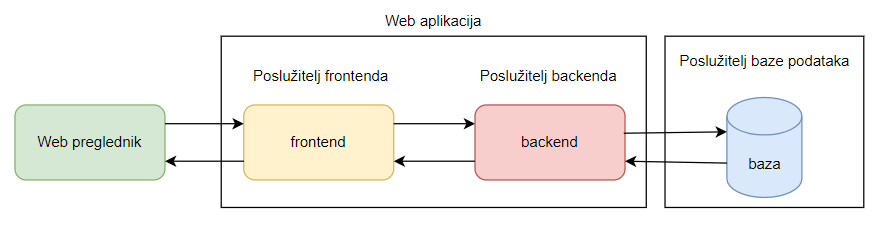
\includegraphics[scale=0.8]{slike/Arhitektura.png} %veličina slike u odnosu na originalnu datoteku i pozicija slike
 			\centering
 			\caption{Arhitektura sustava}
 			\label{fig:arhitektura}
 		\end{figure}
		
		Web preglednik je program koji korisniku omogućuje pregled web-stranica i multimedijskih sadržaja vezanih uz njih. Svaki internetski preglednik je prevoditelj. Korisnik putem web preglednika šalje zahtjev web poslužitelju.
		
		Web poslužitelj osnova je rada web aplikacije. Njegova primarna zadaća je komunikacija s aplikacijom koja se odvija preko HTTPS (engl. Hyper Text Transfer Protocol Secure) protokola, što je protokol u prijenosu informacija na webu. Poslužitelj je onaj koji pokreće web aplikaciju te joj prosljeđuje zahtjev.
		
		Korisnik koristi web aplikaciju za obrađivanje željenih zahtjeva. Web aplikacija obrađuje zahtjev te ovisno o zahtjevu, pristupa bazi podataka nakon čega preko poslužitelja vraća korisniku odgovor u web pregledniku.
		
		Programski jezik kojeg smo odabrale za izradu naše web aplikacije je Java u okviru Spring Boot te programski jezik JavaScript u React razvojnoj biblioteci. Odabrana razvojna okruženja su IntelliJ, Eclipse i  VSCode.
		Arhitektura web aplikacije je slojevita što omogućava nezavisan razvoj pojedinog dijela aplikacije, lakše ispitivanje i održavanje aplikacije te vrlo jednostavno dodavanje novih značajki u sustav. Sastoji se od pristupne i pozadinske aplikacije.
		
		Pristupna aplikacija (frontend) preko Rest API komunicira s pozadinskom aplikacijom.
		
		Pozadinska aplikacija (backend) je troslojno ustrojena:
		\begin{itemize}
		\item Repository
		\item Service
		\item Controller
		\end{itemize}
		Controller predstavlja sloj aplikacije koji obrađuje HTTP zahtjeve i priprema podatke za prikaz u JSON datoteke.
		Service je središnji sloj koji izravno upravlja podatcima, logikom i pravilima aplikacije te obavlja autentikaciju i validaciju.
		Repository šalje SQL upite bazi podataka, odnosno obavlja CRUD (Create, Retrieve, Update and Delete) operacije.
		

				
		\section{Baza podataka}
			
			
			
		Za potrebe našeg sustava koristit ćemo relacijsku bazu podataka čija je gradivna jedinka relacija, odnosno dvodimenzionalna imenovana tablica sa skupom atributa - imenovanim stupcima tablice. Relacijska baza podataka omogućava jednostavno pohranjivanje i upravljanje podatcima. Baza podataka ove aplikacije sastoji se od sljedećih entiteta:
		
		\begin{itemize}
		    \item   UserAccount
		    \item   Conference
		    \item   Multimedia
		    \item   SpecialEvent
		    \item   DataGroup
		    \item   conferenceDataGroup
		    \item   operationalAdmins
		    \item   pending
		    \item   attendees
                \item   users
		\end{itemize}

		
			\subsection{Opis tablica}
			
			\textbf{UserAccount} Ovaj entitet opisuje korisnika konferencije i njegov račun s kojim se prijavljuje u aplikaciju. Sadrži atribute idUserAccount, address, companyName, country, detailsOfParticipation, email, enabled, firstAndLastName, isMainAdmin, isOperativeAdmin, isParticipant, isSystemOwner, phoneNumber, username, password i idConference. Postoje četiri vrste korisnika, vlasnik sustava, glavni admin, operativni admin te sudionik konferencije.
			
		
				
				\begin{longtblr}[
					label=none,
					entry=none
					]{
						width = \textwidth,
						colspec={|X[13,l]|X[9, l]|X[20, l]|}, 
						rowhead = 1,
					} %definicija širine tablice, širine stupaca, poravnanje i broja redaka naslova tablice
					\hline \multicolumn{3}{|c|}{\textbf{UserAccount}}	 \\ \hline[3pt]
					\SetCell{LightGreen}idUserAccount & INT	&  	jedinstveni identifikator korisnika  	\\ \hline
					address	& VARCHAR &  adresa 	\\ \hline 
					companyName & VARCHAR &   ime tvrtke\\ \hline 
					country & VARCHAR	&  		država\\ \hline
					detailsOfParticipation & VARCHAR	&  	uloga	\\ \hline
					email & VARCHAR	&  	email	\\ \hline
                        enabled & BOOLEAN	&  	potvrđen račun	\\ \hline
					firstAndLastName & VARCHAR	&  	ime i prezime	\\ \hline
					isMainAdmin & BOOLEAN	&  	je li glavni admin\\ \hline
					isOperativeAdmin & BOOLEAN	&  je li operativni admin		\\ \hline
					isParticipant & BOOLEAN	& je li participant  		\\ \hline
					isSystemOwner & BOOLEAN	&  je li vlasnik sustava		\\ \hline
					phoneNumber & VARCHAR	&  broj mobitela		\\ \hline
					username & VARCHAR	&  	korisničko ime	\\ \hline
					password & VARCHAR	&  	lozinka	\\ \hline
				\end{longtblr}

                \vspace{8mm}
				
				
				\textbf{Conference} Ovaj entitet opisuje konferenciju. Sadrži atribute idConference, city, country, dateStart, dateEnd, description, topics, name,
				mainAdminIdUserAccount i systemOwnerIdUserAccount. Ovaj entitet je u dvije veze \textit{One-to-Many} sa entitetom UserAccount preko atributa idConference, jedna veza predstavlja operativne admine, a druga participante konferencije, također je u vezi \textit{One-to-Many} sa entitetom dataGroup preko atributa idConference, \textit{One-to-Many} sa entitetom SpecialEvent preko atributa idConference te je u vezi \textit{One-to-Many} sa entitetom Multimedia preko atributa idConference.
			
				
				\begin{longtblr}[
					label=none,
					entry=none
					]{
						width = \textwidth,
						colspec={|X[17,l]|X[7, l]|X[20, l]|}, 
						rowhead = 1,
					} %definicija širine tablice, širine stupaca, poravnanje i broja redaka naslova tablice
					\hline \multicolumn{3}{|c|}{\textbf{Conference}}	 \\ \hline[3pt]
					\SetCell{LightGreen}idConference & INT	&  	jedinstveni identifikator konferencije  	\\ \hline
					city	& VARCHAR & grad u kojem se održava  	\\ \hline 
                        country	& VARCHAR & država u kojoj se održava  	\\ \hline 
                        dateStart	& DATE & datum početka konferencije 	\\ \hline
					dateEnd & DATE &  datum završetka konferencije \\ \hline 
					description	& VARCHAR &  kratak opis konferencije 	\\ \hline
                        topics	& VARCHAR &  teme 	\\ \hline 
					name & VARCHAR &   naziv grupe podaataka\\ \hline 
					\SetCell{LightBlue}mainAdminIdUserAccount & INT &  id glavnog admina sustava \\ \hline 
					\SetCell{LightBlue}systemOwnerIdUserAccount & INT &  id vlasnika sustava \\ \hline 
				\end{longtblr}

                \vspace{8mm}
				
				
				\textbf{Multimedia} Ovaj entitet opisuje multimedijske sadržaje snimane od strane ovlaštenog fotografa za određenu konferenciju. Sadrži atribute idMultimedia, url, date i idConference.  Ovaj entitet je u vezi \textit{Many-to-One} sa entitetom Conference preko atributa idConference.
				
				\begin{longtblr}[
					label=none,
					entry=none
					]{
						width = \textwidth,
						colspec={|X[7,l]|X[6, l]|X[20, l]|}, 
						rowhead = 1,
					} %definicija širine tablice, širine stupaca, poravnanje i broja redaka naslova tablice
					\hline \multicolumn{3}{|c|}{\textbf{Multimedia}}	 \\ \hline[3pt]
					\SetCell{LightGreen}idMultimedia & INT	&  	jedinstveni identifikator multimedijskog sadržaja  	\\ \hline
					url	& VARCHAR &  link na drive gdje je pohranjena multimedia	\\ \hline 
					date	& DATETIME &   datum nastanka	\\ \hline 
					\SetCell{LightBlue}idConference	& INT &   id konferencije kojoj pripada	\\ \hline 
				\end{longtblr}

                \vspace{8mm}
				
				
				
				\textbf{SpecialEvent} Ovaj entitet opisuje posebna događanja tijekom neke konferencije. Sadrži atribute idSpecialEvent, capacity, type, message i idConference.  Ovaj entitet je u vezi \textit{Many-to-One} sa entitetom Conference preko atributa idSpecialEvent te je u dvije veze \textit{Many-to-Many} sa entitetom UserAccount preko atributa idSpecialEvent. Jedna veza opisuje korisnike koji su prijavljeni za sudjelovanje na posebnom događaju, a druga opisuje korisnike koji su na čekanju za sudjelovanje zbog popunjenih kapaciteta.
			
				
				\begin{longtblr}[
					label=none,
					entry=none
					]{
						width = \textwidth,
						colspec={|X[7,l]|X[6, l]|X[20, l]|}, 
						rowhead = 1,
					} %definicija širine tablice, širine stupaca, poravnanje i broja redaka naslova tablice
					\hline \multicolumn{3}{|c|}{\textbf{SpecialEvent}}	 \\ \hline[3pt]
					\SetCell{LightGreen}idSpecialEvent & INT	&  	jedinstveni identifikator posebnog događaja 	\\ \hline
					capacity	& INT &   maksimalan broj sudionika	\\ \hline 
					type & VARCHAR &  tip događaja \\ \hline 
					message & VARCHAR &  kratka poruka o događaju \\ \hline 
                        \SetCell{LightBlue}idConference	& INT &   id konferencije kojoj pripada	\\ \hline 
				\end{longtblr}

                \vspace{8mm}
				
				
				\textbf{DataGroup} Ovaj entitet opisuje grupu podataka o nekoj konferenciji (raspored, zbornik radova i sl.). Sadrži atribute idDataGroup, groupName, data i idConference.  Ovaj entitet je u vezi \textit{Many-to-One} sa entitetom Conference preko atributa idDataGroup.
				
				\begin{longtblr}[
					label=none,
					entry=none
					]{
						width = \textwidth,
						colspec={|X[10,l]|X[6, l]|X[20, l]|}, 
						rowhead = 1,
					} %definicija širine tablice, širine stupaca, poravnanje i broja redaka naslova tablice
					\hline \multicolumn{3}{|c|}{\textbf{DataGroup}}	 \\ \hline[3pt]
					\SetCell{LightGreen}idDataGroup & INT	&  	jedinstveni identifikator grupe podataka  	\\ \hline
					data	& VARCHAR &   	podatak za određenu grupu podataka (može biti tekst ili datoteka)\\ \hline 
					groupName	& VARCHAR &   	naziv\\ \hline
				\end{longtblr}

                \vspace{8mm}
				
				
				
				\textbf{ConferenceDataGroup} Ovaj entitet opisuje odnos između entiteta Conference i DataGroup. Sadrži atribute idDataGroup i idConference.  Ovaj entitet je u vezi \textit{Many-to-One} sa entitetom Conference preko atributa idConference te u vezi \textit{Many-to-One} sa entitetom DataGroup preko atributa idDataGroup.
				
				\begin{longtblr}[
					label=none,
					entry=none
					]{
						width = \textwidth,
						colspec={|X[13,l]|X[6, l]|X[20, l]|}, 
						rowhead = 1,
					} %definicija širine tablice, širine stupaca, poravnanje i broja redaka naslova tablice
					\hline \multicolumn{3}{|c|}{\textbf{ConferenceDataGroup}}	 \\ \hline[3pt]
					\SetCell{LightGreen}idDataGroup & INT	&  	jedinstveni identifikator grupe podataka  	\\ \hline
					\SetCell{LightGreen}idConference	& INT &   jedinstveni identifikator konferencije   	\\ \hline
				\end{longtblr}

                \vspace{8mm}
				
				\textbf{OperationalAdmins} Ovaj entitet opisuje odnos između entiteta Conference i UserAccount, a predstavlja operativne admine. Sadrži atribute idUserAccount i idConference.  Ovaj entitet je u vezi \textit{Many-to-One} sa entitetom Conference preko atributa idConference te u vezi \textit{Many-to-One} sa entitetom UserAccount preko atributa idUserAccount.
				
				\begin{longtblr}[
					label=none,
					entry=none
					]{
						width = \textwidth,
						colspec={|X[17,l]|X[6, l]|X[20, l]|}, 
						rowhead = 1,
					} %definicija širine tablice, širine stupaca, poravnanje i broja redaka naslova tablice
					\hline \multicolumn{3}{|c|}{\textbf{OperationalAdmins}}	 \\ \hline[3pt]
					\SetCell{LightGreen}idUserAccount & INT	&  	jedinstveni identifikator operativnog admina  	\\ \hline
					\SetCell{LightGreen}idConference	& INT &   jedinstveni identifikator konferencije   	\\ \hline
				\end{longtblr}

                \vspace{8mm}
				
				
				\textbf{Users} Ovaj entitet opisuje odnos između entiteta Conference i UserAccount, a predstavlja participante konferencije. Sadrži atribute idUserAccount i idConference.  Ovaj entitet je u vezi \textit{Many-to-One} sa entitetom Conference preko atributa idConference te u vezi \textit{Many-to-One} sa entitetom UserAccount preko atributa idUserAccount.
				
				\begin{longtblr}[
					label=none,
					entry=none
					]{
						width = \textwidth,
						colspec={|X[17,l]|X[6, l]|X[20, l]|}, 
						rowhead = 1,
					} %definicija širine tablice, širine stupaca, poravnanje i broja redaka naslova tablice
					\hline \multicolumn{3}{|c|}{\textbf{Users}}	 \\ \hline[3pt]
					\SetCell{LightGreen}idUserAccount & INT	&  	jedinstveni identifikator participanta konferencije  	\\ \hline
					\SetCell{LightGreen}icConference	& INT &   jedinstveni identifikator konferencije   	\\ \hline
				\end{longtblr}

                \vspace{8mm}

                
				\textbf{VerificationToken} Ovaj entitet opisuje tokene koji se koriste pri potvrdi računa mailom. Ovaj entitet je u vezi \textit{Many-to-One} sa entitetom UserAccount preko atributa idUserAccount.
				
				\begin{longtblr}[
					label=none,
					entry=none
					]{
						width = \textwidth,
						colspec={|X[17,l]|X[8, l]|X[20, l]|}, 
						rowhead = 1,
					} %definicija širine tablice, širine stupaca, poravnanje i broja redaka naslova tablice
					\hline \multicolumn{3}{|c|}{\textbf{VerificationToken}}	 \\ \hline[3pt]
					\SetCell{LightGreen}idToken & INT	&  	jedinstveni identifikator tokena  	\\ \hline
					createdDate	& DATE &   datum i vrijeme nastanka tokena   	\\ \hline
                        expiryDate	& DATE &   datum i vrijeme prestanka valjanosti tokena   	\\ \hline
                        token	& VARCHAR &   token   	\\ \hline
                        \SetCell{LightBlue}idUserAccount	& INT &   id korisničkog računa za kojeg je token generiran   	\\ \hline
				\end{longtblr}

                \vspace{8mm}

                
            


                \textbf{SpecialEventAttendees} Ovaj entitet opisuje odnos između entiteta SpecialEvent i UserAccount, a predstavlja participante koji su prijavljeni na neki specijalni događaj. Sadrži atribute idUserAccount i idSpecialEvent.  Ovaj entitet je u vezi \textit{Many-to-One} sa entitetom SpecialEvent preko atributa idSpecialEvent te u vezi \textit{Many-to-One} sa entitetom UserAccount preko atributa idUserAccount.
				
				\begin{longtblr}[
					label=none,
					entry=none
					]{
						width = \textwidth,
						colspec={|X[17,l]|X[6, l]|X[20, l]|}, 
						rowhead = 1,
					} %definicija širine tablice, širine stupaca, poravnanje i broja redaka naslova tablice
					\hline \multicolumn{3}{|c|}{\textbf{SpecialEventAttendees}}	 \\ \hline[3pt]
					\SetCell{LightGreen}idUserAccount & INT	&  	jedinstveni identifikator participanta konferencije  	\\ \hline
					\SetCell{LightGreen}idSpecialEvent	& INT &   jedinstveni identifikator specijalnog događaja   	\\ \hline
				\end{longtblr}

                \vspace{8mm}


                \textbf{SpecialEventPending} Ovaj entitet opisuje odnos između entiteta SpecialEvent i UserAccount, a predstavlja participante koji su se htjeli prijaviti na specijalni događaj, ali su stavljeni na čekanje zbog popunjenih kapaciteta na tom događaju. Sadrži atribute idUserAccount i idSpecialEvent.  Ovaj entitet je u vezi \textit{Many-to-One} sa entitetom SpecialEvent preko atributa idSpecialEvent te u vezi \textit{Many-to-One} sa entitetom UserAccount preko atributa idUserAccount.
				
				\begin{longtblr}[
					label=none,
					entry=none
					]{
						width = \textwidth,
						colspec={|X[17,l]|X[6, l]|X[20, l]|}, 
						rowhead = 1,
					} %definicija širine tablice, širine stupaca, poravnanje i broja redaka naslova tablice
					\hline \multicolumn{3}{|c|}{\textbf{SpecialEventPending}}	 \\ \hline[3pt]
					\SetCell{LightGreen}idUserAccount & INT	&  	jedinstveni identifikator participanta konferencije  	\\ \hline
					\SetCell{LightGreen}idSpecialEvent	& INT &   jedinstveni identifikator specijalnog događaja   	\\ \hline
				\end{longtblr}

                \vspace{8mm}
				
				
				
				
			\subsection{Dijagram baze podataka}
				\begin{figure}[H]
			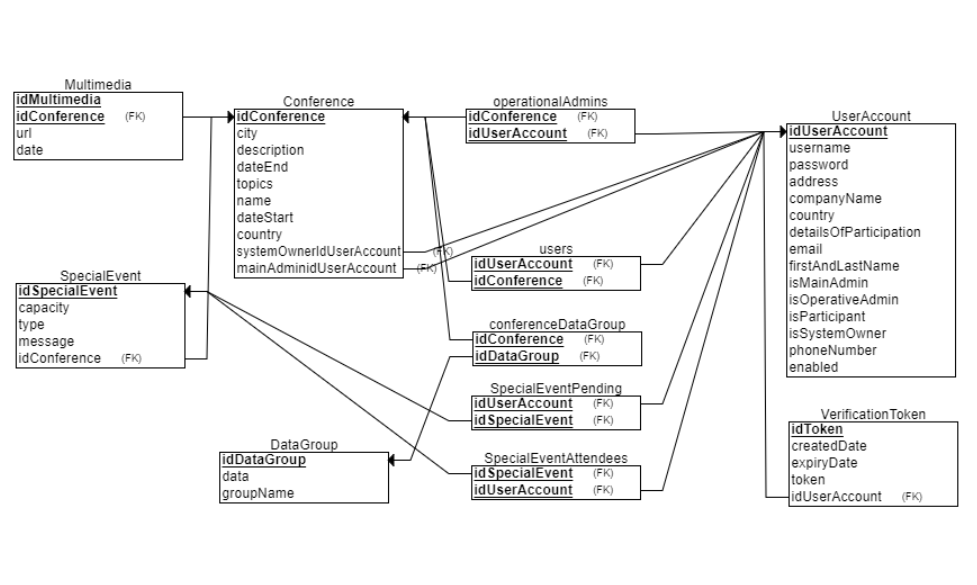
\includegraphics[scale=0.85]{slike/RelModel.PNG} %veličina slike u odnosu na originalnu datoteku i pozicija slike
			\centering
			\caption{Relacijski model baze}
			\label{fig:promjene}
		\end{figure}
			
			\eject
			
			
		
			\section{Dijagram razreda}

			\text Na slikama 4.3, 4.4, 4.5 i 4.6 su prikazani razredi koji pripadaju backend dijelu arhitekture. Slika 4.3 prikazuje razred DTO \textit{(Data Transfer Object)} razrede.
			Na slici 4.4. prikazan je dijagram Modela, oni predstavljaju entitete naše baze podataka, na tom dijagramu također možemo vidjeti i međusobnu ovisnost entiteta. Zatim slike 4.5 i 4.6 prikazuju Kontrolere i Service, metode u Kontrolerima manipuliraju s DTO podatcima, primaju zahtjeve s frontend-a koje dalje šalje na Service gdje se zahtjev obrađuje. Povratna informacija koja se generira u Service se ponovno vraća preko Kontrolera koji vraća JSON datoteku na frontend. 
			

			\begin{figure}[H]
			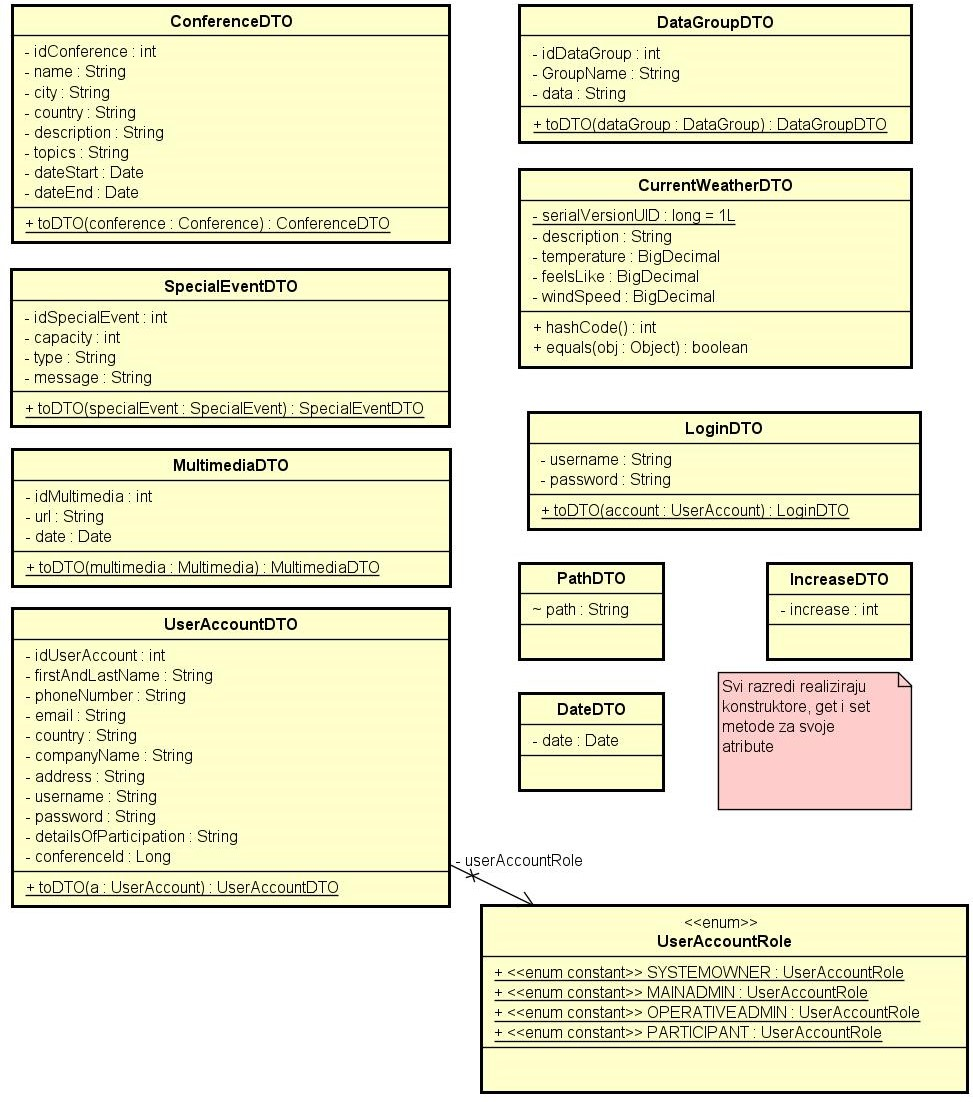
\includegraphics[width=\textwidth]{slike/DTO Dijagram.jpg}
			\centering
			\caption{Dijagram razreda - DTO}
			\label{fig:}
			\end{figure}
			
			\newpage

			\begin{figure}[H]
			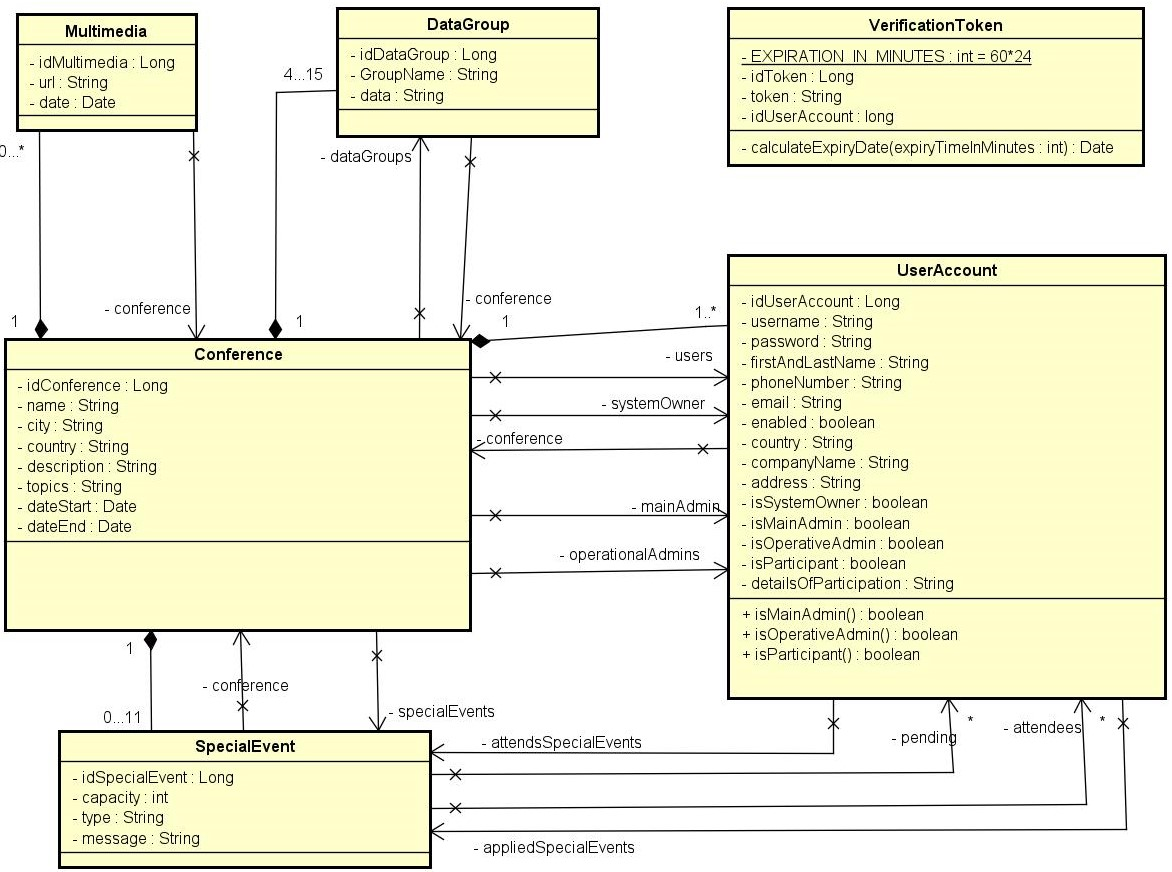
\includegraphics[width=\textwidth]{slike/Model diagram.jpg}
			\centering
			\caption{Dijagram razreda - Modeli}
			\label{fig:dijagram_razreda_modeli}
			\end{figure}
			
			\newpage


			\begin{figure}[H]
			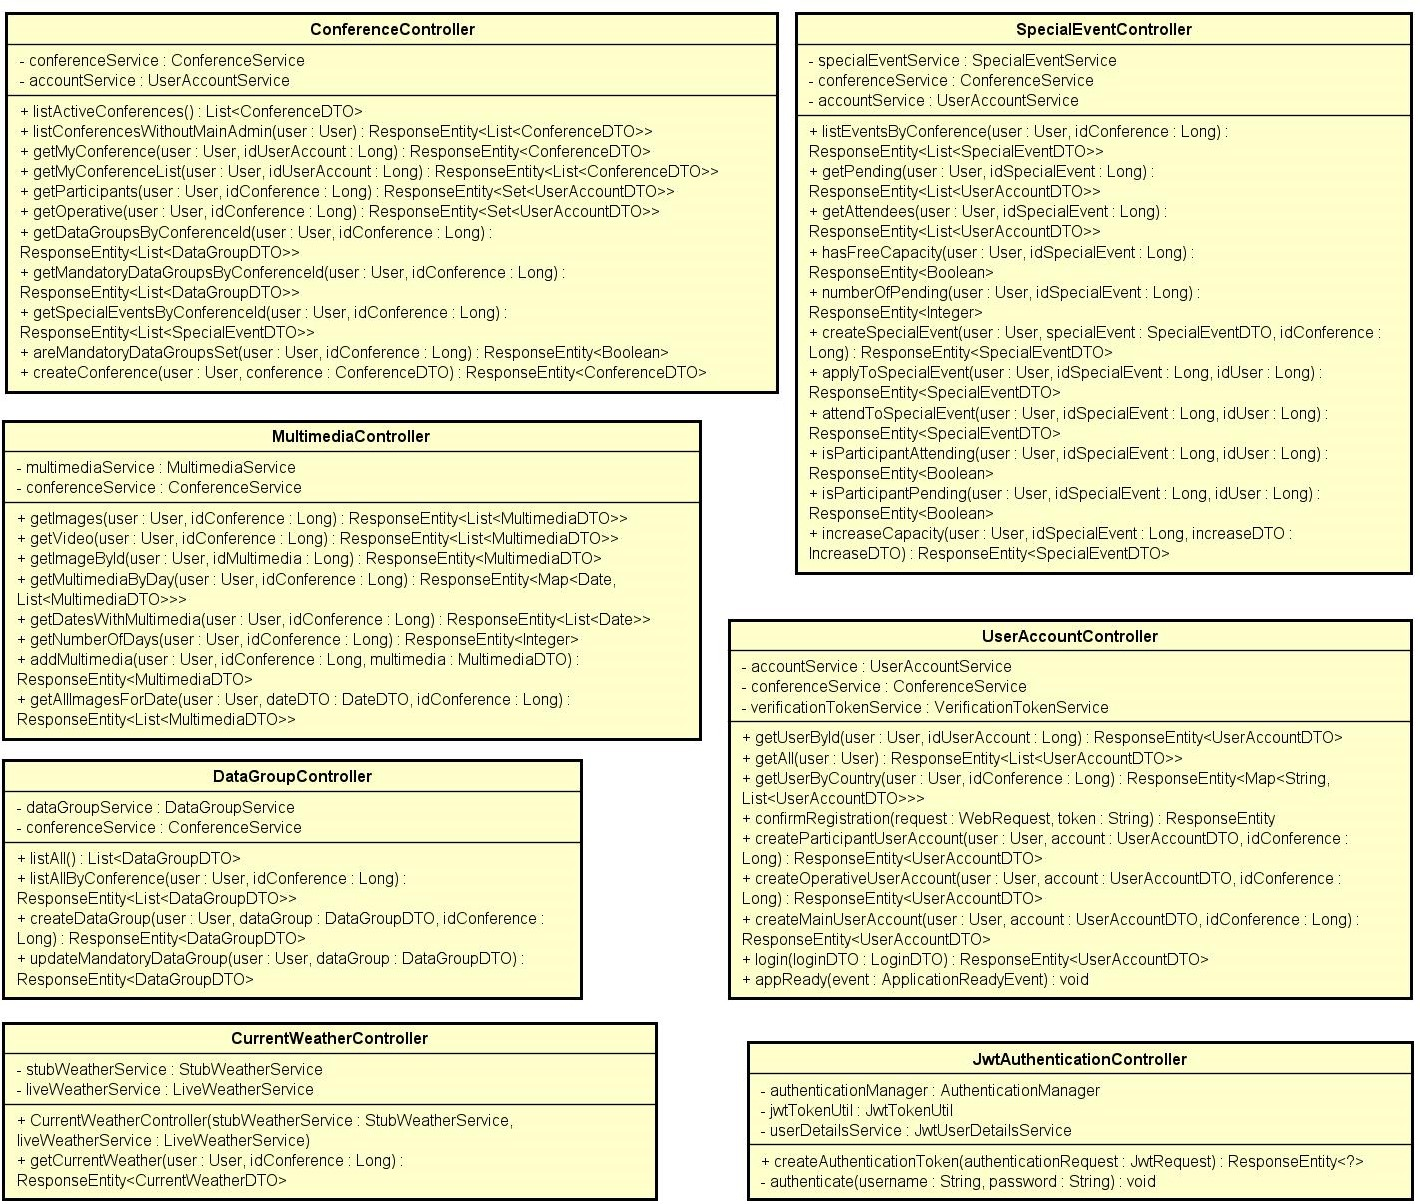
\includegraphics[width=\textwidth]{slike/Controller Dijagram.jpg}
			\centering
			\caption{Dijagram razreda - Kontroleri}
			\label{fig:dijagram_razreda_kontroleri}
			\end{figure}
			
			\newpage

			 \begin{figure}[H]
			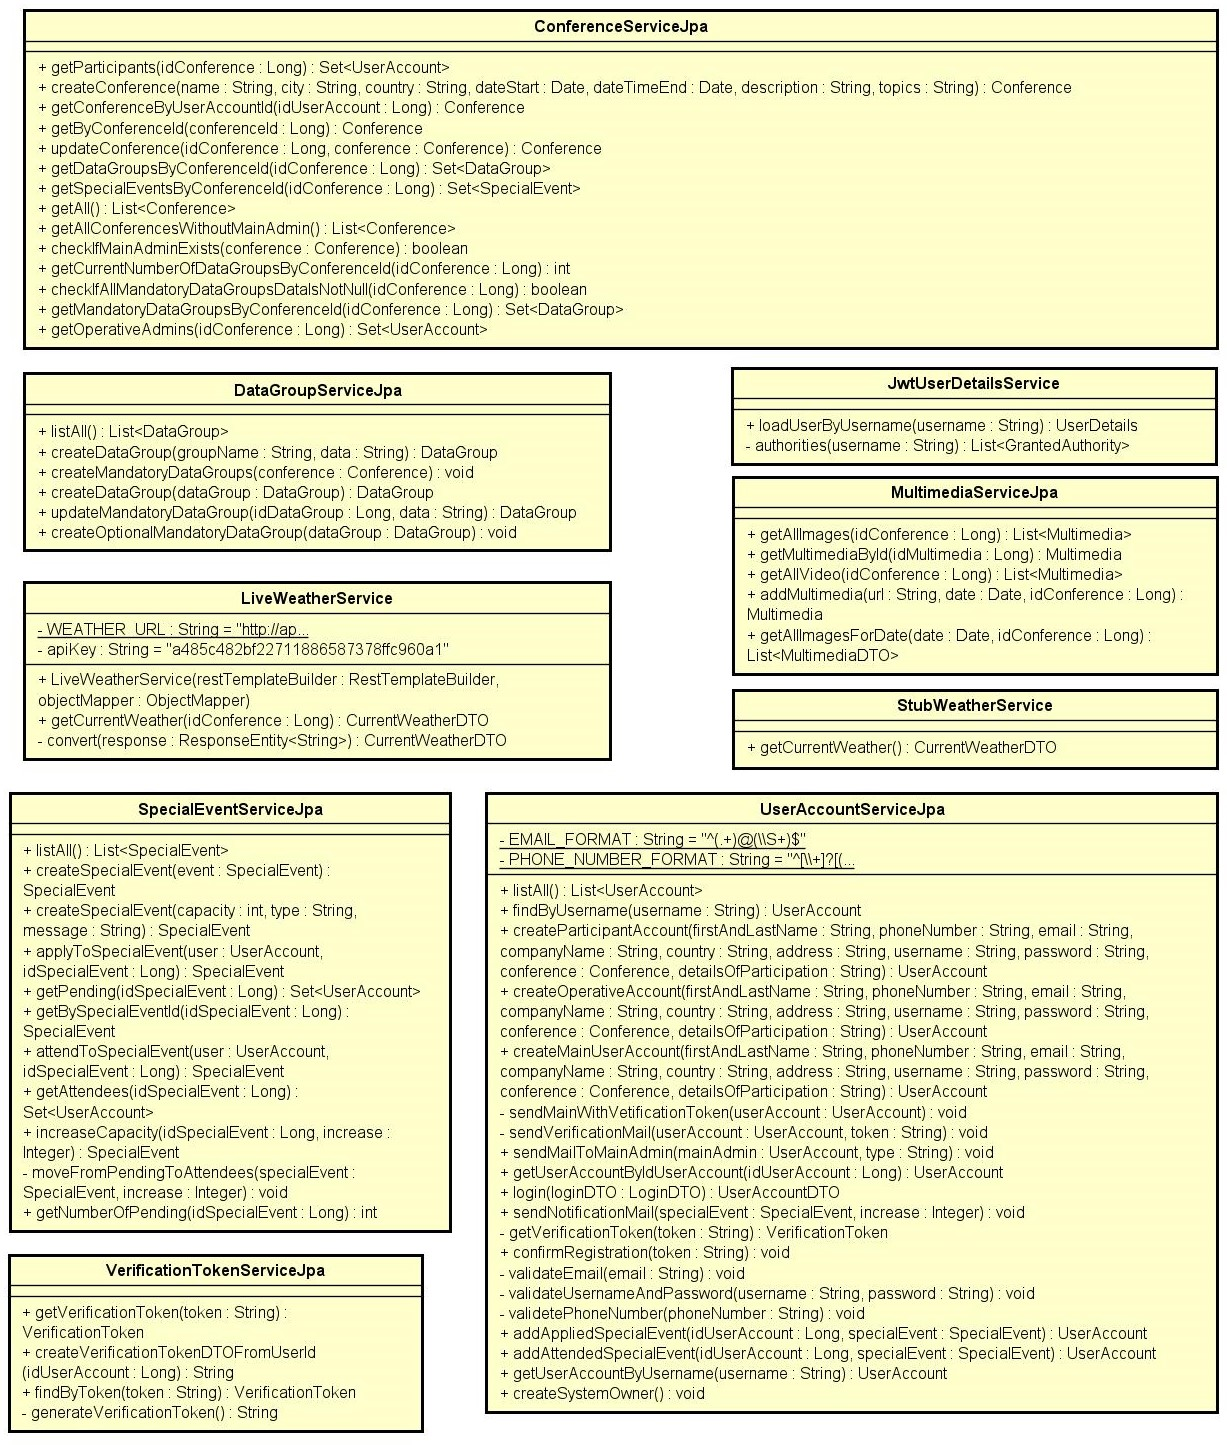
\includegraphics[width=\textwidth]{slike/ServiceImpl Dijagram.jpg}
			\centering
			\caption{Dijagram razreda -  Service}
			\label{fig:dijagram_razreda_service}
			\end{figure}
			
			\newpage
			
	
			\eject
		
		\section{Dijagram stanja}
			
			
Dijagram stanja prikazuje stanja objekta te prijelaze iz jednog stanja u drugo temeljene na dogadajima. Na slici 4.7 prikazan je dijagram stanja za registriranog main admina. Nakon prijave prvo se prikazuje početni izbornik koji nudi tri opcije : \textit{Home, My Conference} i \textit{Create Operative Admin}. Klikom na "Home" poziva se početna stranica na kojoj se prikazuju aktivne konferencije. Klikom na "Create Operative Admin" prikaže se forma za kreiranje operativnog admina. Klikom na \"My Conference" prikažu se podatci o konferenciji. Main admin tu ima mogućnosti stvoriti novu grupu podataka klikom na "New Data Group". Ima mogućnsot pregleda svih sudionika i operativnih admina klikom na \textit{Show Attendees}. Klikom na "Special Events" main admin dobiva prikaz svih događaja za tu konferenciju gdje može odabrati stvaranje novog događaja klikom na "New Special Event". Također može povećati kapacitet za određeni događaj. Ako je lista čekanja prazna, povećanje kapaciteta će biti odbijeno, ako lista čekanja nije prazna kapacitet će se povećati. Iz stanja \textit{Prikaz Moje Konferencije} može pristupiti i multimediji klikom na "See Multimedia", dobiva prikaz direktorija raspoređeni po danima, klikom na direktorij prikažu se slike tog dana.

                \begin{figure}[H]
			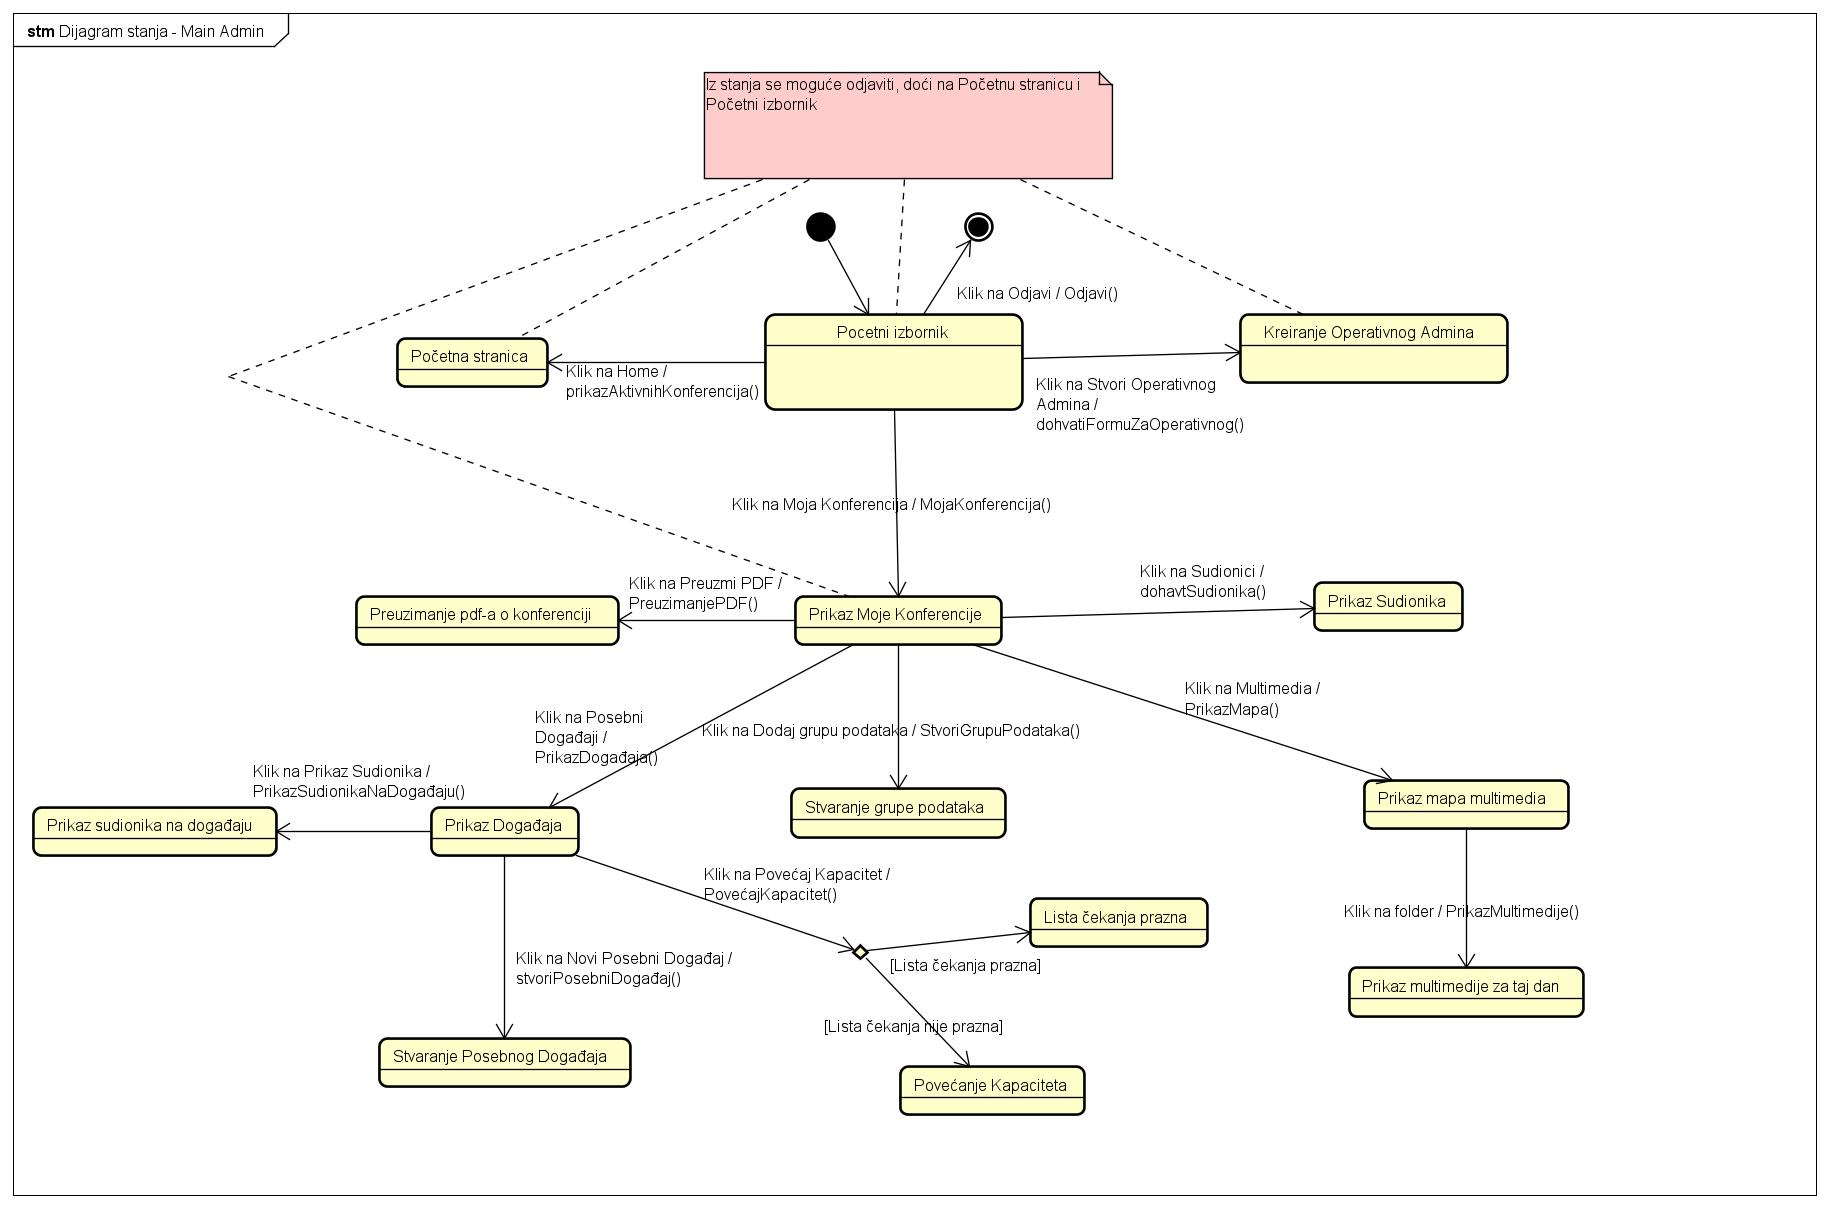
\includegraphics[width = \textwidth]{slike/Dijagram stanja - Main Admin.jpg}
			\centering
			\caption{Dijagram stanja - Main Admin}
			\label{fig:dijagram-stanja-main-admin}
			\end{figure}
			
			
			\eject 
		
			\section{Dijagram aktivnosti}
			
			\textbf{Vlasnik sustava - kreiranje konferencije i glavnog admina}\\

		   \text Na dijagramu aktivnosti prikazan je proces stvaranja konferencije i main admina. Vlasnik sustava prijavljuje se u sustav, odabire gumb za kreiranje konferencije, te unosi podatke o konferenciji. Nakon toga otvara se obrazac za unos podataka o main adminu.


		   \begin{figure}[H]
		   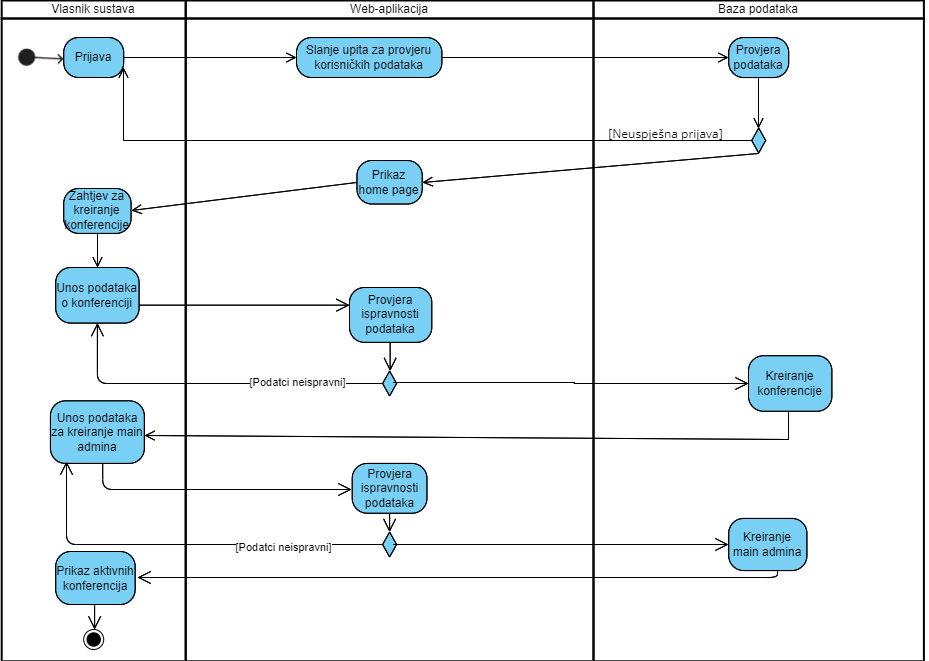
\includegraphics[scale=0.65]{slike/Dijagram aktivnosti - system owner.png} %veličina
		   
		   \centering
		   \caption{Kreiranje konferencije i glavnog admina}
		   \label{fig:dijagram_aktivnosti_vlasnik_sustava}
		   \end{figure}

  \textbf{Glavni admin - unos grupa podataka}\\

		   \text Na dijagramu aktivnosti prikazan je proces unosa grupa podataka. Glavni admin prijavljuje se u sustav, odabire gumb "My conference", te unosi obavezne grupe podataka. Nakon toga može stvarati i opcionalne grupe po dataka. 


		   \begin{figure}[H]
		   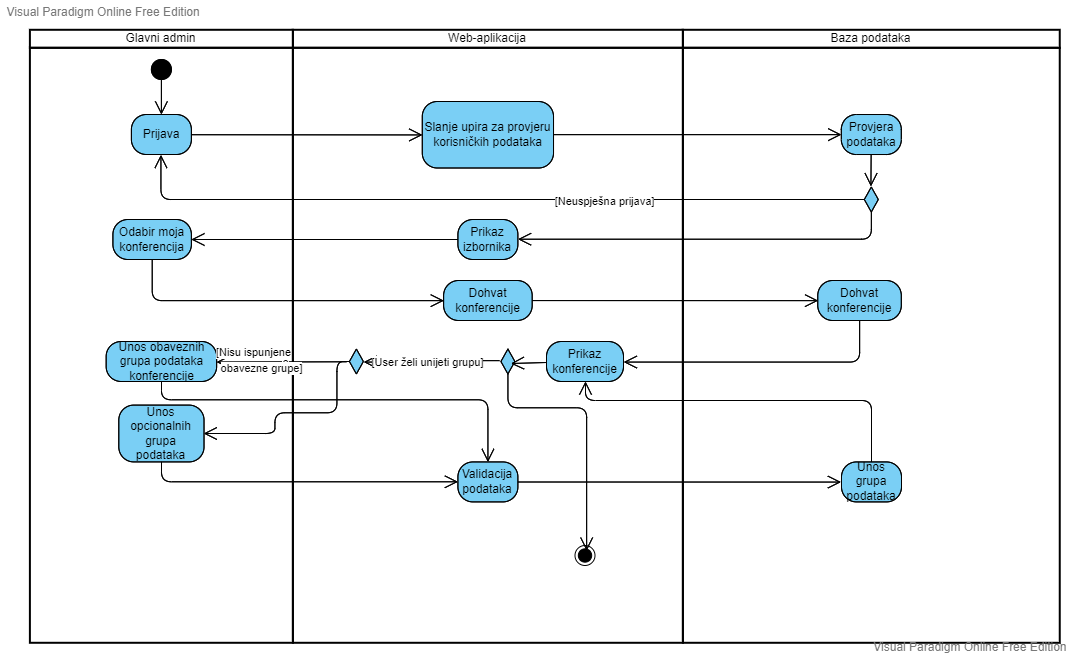
\includegraphics[scale=0.45]{slike/Main admin - unos grupa podataka.png} %veličina
		   
		   \centering
		   \caption{Unos grupa podataka}
		   \label{fig:dijagram_aktivnosti_glavni_admin}
		   \end{figure}

   \textbf{Operativni admin - kreiranje korisnika}\\

		   \text Na dijagramu aktivnosti prikazan je proces kreiranja korisnika. Operativni admin prijavljuje se u sustav, odabire gumb "Create user", te mu se otvara obrazac za popunjavanje podataka o korisniku. Nakon uspješnog unosa korisnika, korisnik mora potvrditi svoj korisnički račun mailom.  


		   \begin{figure}[H]
		   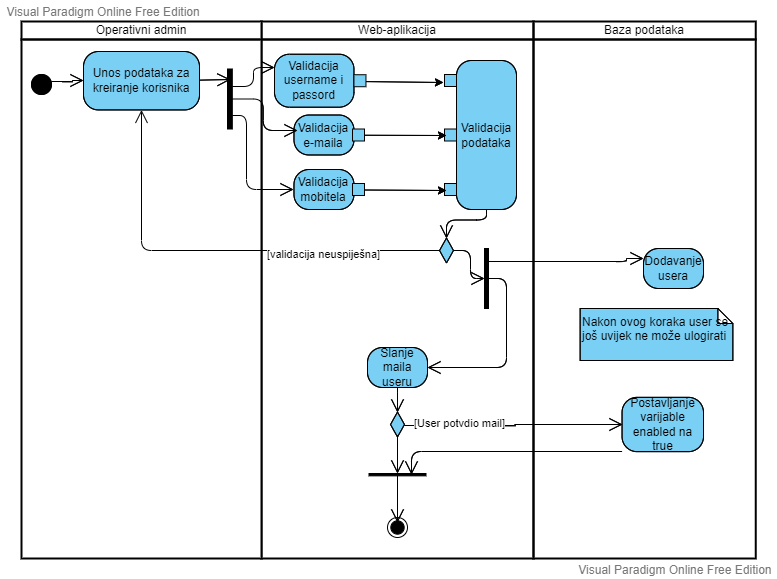
\includegraphics[scale=0.60]{slike/Creating user.vpd.png} %veličina
		   
		   \centering
		   \caption{Kreiranje korisnika}
		   \label{fig:dijagram_aktivnosti_operativni_admin}
		   \end{figure}

  \textbf{Korisnik - prijava na specijalni event}\\

		   \text Na dijagramu aktivnosti prikazan je proces prijave korisnika na specijalni event. Kada korisnik odabere gumb "Special event", otvara mu se lista specijalnih eventova na koje se može prijaviti. Ako na na specijalnom eventu ima mjesta, korisnik se automatski dodaje na listu prijavljenih korisnika za specijalni event. U slučaju da su sva mjesta na specijalnom eventu popunjena, korisnika se o tome obavještava. U slučaju da se naknadno poveća broj slobodnih mjesta na specijalnom eventu, korisnika se mailom obavještava da je sada na listi prijavljenih korisnika.  


		   \begin{figure}[H]
		   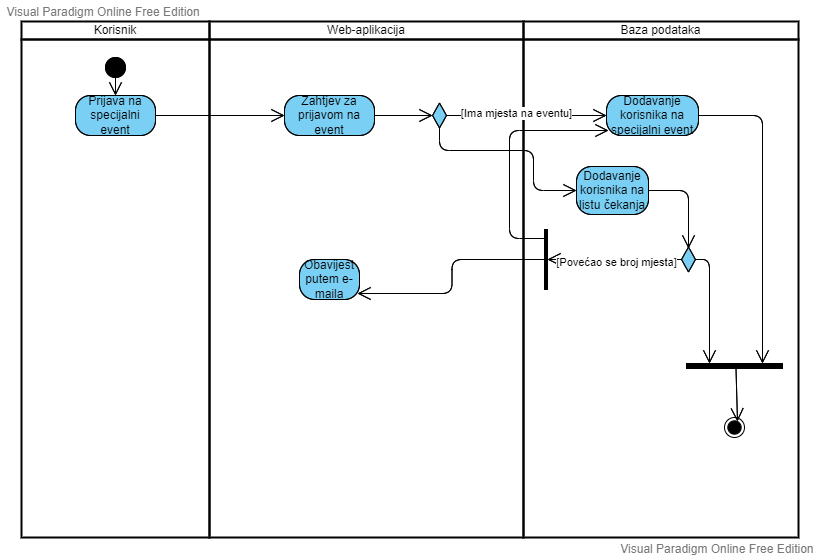
\includegraphics[scale=0.55]{slike/Prijava na special event.vpd.png} %veličina
		   
		   \centering
		   \caption{Prijava na specijalni event}
		   \label{fig:dijagram_aktivnosti_korisnik}
		   \end{figure}
		   
		   
		   \eject

		\section{Dijagram komponenti}

     \textbf{Dijagram komponenti}\\
				
				{Prikazani dijagram komponenti prikazuje organizaciju i međuovisnost komponenti i odnose prema okolini. Sustavu se pristupa preko dva različita sučelja. Preko sučelja za dohvat HTML, CSS i JS datoteka poslužuju se datoteke koje pripadaju frontend dijelu aplikacije. To je sučelje zahtjevano sučelje za React View komponentu budući da preko njega ostvaruje prikaz i osvježavanje frontenda. Router je komponenta koja na upit s url-om određuje koja datoteka će se poslužiti na sučelje. Svaka datoteka predstavlja jednu stranicu aplikacije, tj. JavaScript kod te datoteke. Sve JavaScript datoteke ovise o React biblioteci iz koje dohvaćaju gotove komponente kao što su gumbi, forme i slično. Preko sučelja za dohvat JSON podataka pristupa se REST API komponenti. REST API poslužuje podatke koji pripadaju backend dijelu aplikacije. JPA(Java persistance API) je zadužen za dohvaćanje tablica iz baze podataka pomoću SQL upita. Sučelje za komunikaciju s JPA koristi Repository razred Swing aplikacije kako bi na zahtjev iz Service komponente mogla poslati upit bazi podataka. Podatci koji su pristigli iz baze se šalju dalje arhitekturi u obliku DTO (Data transfer object) iz Service prema Contolleru i dalje prema frontend dijelu aplikacije. Reactview komponenta preko dostupnih sučelja komunicira sa Kokeferencije aplikacijom te ovisno o korisnikovim akcijama osvježava prikaz i dohvaća nove podatke ili datoteke.}
				
		        \begin{figure}[H]
			            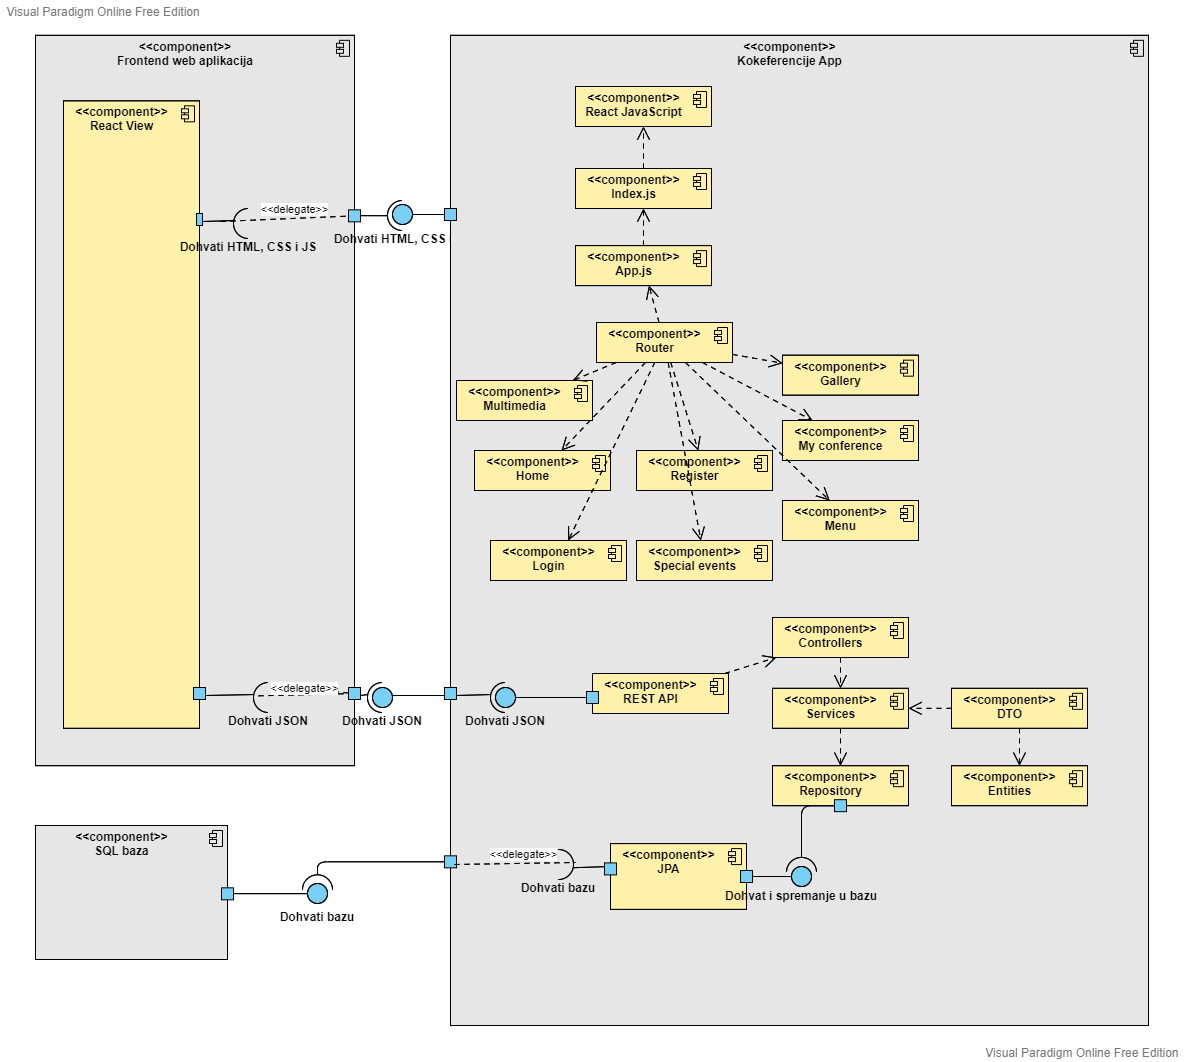
\includegraphics[scale=0.40]{slike/Dijagram_komp.png} %veličina slike u odnosu na originalnu datoteku i pozicija slike
			            \centering
			            \caption{Dijagram komponenti}
			            \label{fig:seq-dijagram2}
		        \end{figure}\\
				\eject
	\chapter{Implementacija i korisničko sučelje}
		
		
		\section{Korištene tehnologije i alati}
		
		Tim je komunicirao putem aplikacija WhatsApp\footnote{\url{https://www.whatsapp.com/}} te Discord\footnote{\url{https://discord.com/}}. WhatsApp je besplatna aplikacija za dopisivanje te je prvenstveno služila za međusobne dogovore kao i razrješavanje pojedinih nejasnoća. Discord je  aplikacija i platforma za digitalnu distribuciju, dizajnirana prvenstveno za zajednice koje se bave igranjem video igara. Specijalizirana je za tekstualnu, slikovnu, video i audio komunikaciju između korisnika što je uvelike olakšalo komunikaciju prilikom procesa izrade aplikacije. Za izradu UML dijagrama korišten je alat Astah Professional\footnote{\url{https://astah.net/products/astah-professional/}} te Visual Paradigm\footnote{\url{https://www.visual-paradigm.com/}}. Kao sustav za upavljanje izvornim kodom koristio se Git\footnote{\url{https://git-scm.com/}}, a udaljeni repozitorij projekta je dostupan na web platformi Gitlab\footnote{\url{https://gitlab.com/}}.
		\newline

Kao razvojna okruženja korišteni su IntelliJ IDEA\footnote{\url{https://www.jetbrains.com/idea/}}, Eclipse\footnote{\url{https://www.eclipse.org/}} te Microsoft Visual Studio\footnote{\url{https://visualstudio.microsoft.com/}}. IntelliJ IDEA je integrirano razvojno okruženje (IDE) napisano u Javi za razvoj računalnog softvera napisanog u Javi, Kotlinu, Groovyju i drugim jezicima koji se temelje na JVM-u. Razvio ga je JetBrains (ranije poznat kao IntelliJ) i dostupan je kao Apache 2 licencirano izdanje zajednice i u vlasničkom komercijalnom izdanju. Oba se izdanja mogu koristiti za komercijalni razvoj. Eclipse je integrirano razvojno okruženje koje se koristi u računalnom programiranju. Sadrži osnovni radni prostor i proširivi sustav za prilagođavanje okruženja. To je drugi najpopularniji IDE za Java razvoj, a do 2016. bilo je najpopularniji. Visual Studio je integrirano razvojno okruženje tvrtke Microsoft. Koristi se za razvoj računalnih programa uključujući web stranice, web aplikacije, web usluge i mobilne aplikacije.
		\newline

Aplikacija je napisana pomoću radnog okvira Spring framework\footnote{\url{https://spring.io/projects/spring-framework}} i jezika Java\footnote{\url{https://www.java.com/en/}} za izradu \textit{backenda}, a za izradu \textit{frontenda} koristio se React\footnote{\url{https://reactjs.org/}} te jezik Javascript\footnote{\url{https://www.javascript.com/}}. Spring framework omogućava jednostavan razvoj modernih aplikacija u Javi. Nudi brojne značajke koje su organizirane u module. Središnji modul je Spring spremnik čija je dužnost povezivanje, konfiguriranje, stvaranje i upravljanje životnim ciklusom pojedinog objekta, tj. Spring bean-a. Za razvoj web aplikacija veliku važnost ima Spring MVC modul. On kombinira sve prednosti \textit{Model-View-Controller} obrasca i Spring okvira. Osim Spring modula postoje i Spring projekti, a oni nude sve značajke za određenu funkcionalnost. React je Javascript biblioteka otvorenog koda koja se temelji na lakšem dizajniranju sučelja. Odgovoran je za prikaz slojeva u aplikaciji, a napravio ga je Facebook. React omogućuje programiranje i razvoj aplikacija te je važan dio za  \textit{frontend} development.
	\newline

Za razvoj i testiranje HTTP REST API-ja korišten je alat Postman\footnote{\url{https://www.postman.com/}}, a baza podataka se prije procesa \textit{deploymenta} nalazila lokalno što je ostvareno pomoću PostgreSQL-a\footnote{\url{https://www.postgresql.org/}}, sustava za upravljanje relacijskom bazom podataka otvorenog koda. Nakon \textit{deploymenta} baza podataka se nalazi na poslužitelju u oblaku Render\footnote{\url{https://render.com/}}.
			
			\eject 
		
	
		\section{Ispitivanje programskog rješenja}
			
	
			
			\subsection{Ispitivanje komponenti}

   
			\textbf{Ispitni slučaj 1: Login sa postojećim i nepostojećim korisnikom, te korisnikom čija konferencija više nije dostupna. }
   
   \textbf{Ulaz:}
   \begin{packed_item}
   \item[] \begin{packed_enum}
				
				\item Username i password postojećeg korisnika
    \item Username i password nepostojećeg korisnika
    \item Username i password korisnika čija konferencije više nije dostupna
				
			\end{packed_enum}
   \end{packed_item}

   \textbf{Očekivani rezultat:}
   \begin{packed_item}
   \item[] \begin{packed_enum}
				
				\item Login je uspješan za postojećeg korisnika i kao odgovor se vraća korisnički račun usera.
    \item Login je neuspješan za nepostojećeg korisnika i kao odgovor se vraća Unauthorised.
    \item Login je neuspješan za korisnika čija je konferencija nedostupna i odgovor je Forbidden.
				
			\end{packed_enum}
   \end{packed_item}
   \textbf{Rezultat:} \text Svaki očekivani rezultat je ostvaren. \color{red} Aplikacija je prošla test. \color{black}

    \begin{figure}[H]
            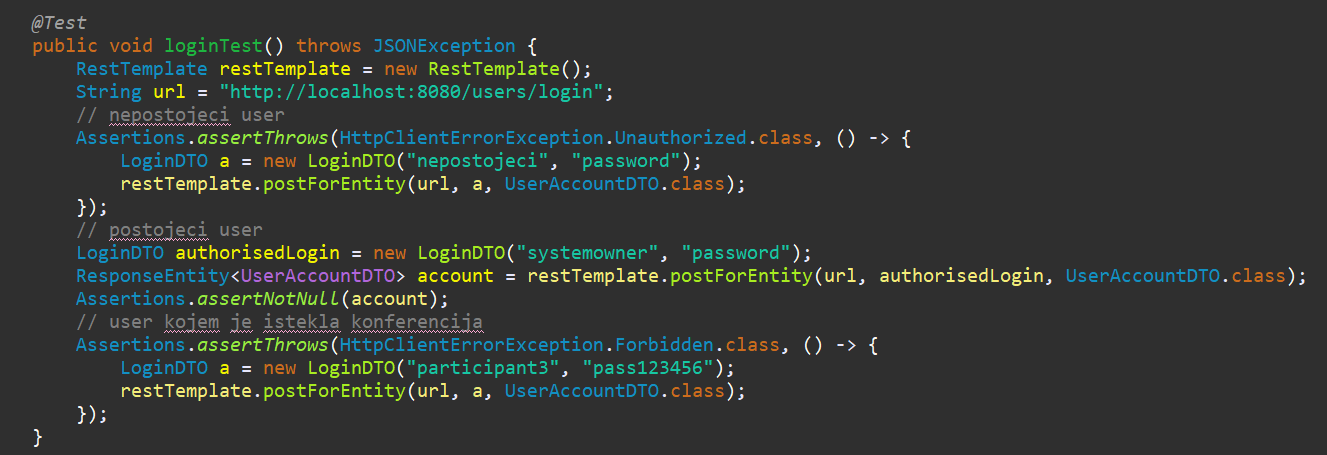
\includegraphics[scale=0.55]{slike/login.png} %veličina
			
			\centering
			\caption{Testiranje prijave}
			\label{fig:testiranje prijave}
			\end{figure}






   \textbf{\newline Ispitni slučaj 2: Registracija korisnika\newline  }
   \textbf{Ulaz:}
   \begin{packed_item}
   \item[] \begin{packed_enum}
				
				\item Stvaranje konferencije te unos ispravnih podataka o korisniku.
    \item Stvaranje konferencije, te unos neispravnih podataka za korisnika (neispravni format e-maila, neispravan format broja mobitela, nedovoljan broj znakova za username, nedovoljan broj znakova za password itd.).
				
			\end{packed_enum}
   \end{packed_item}

   \textbf{Očekivani rezultat:}
   \begin{packed_item}
   \item[] \begin{packed_enum}
				
				\item Registracija je uspješna i kao odgovor se vraća stvoreni korisnički račun.
    \item Registracija je neuspješna te se kao odgovor vraća BadRequest.
				
			\end{packed_enum}
   \end{packed_item}
   \textbf{Rezultat:} \text Svaki očekivani rezultat je ostvaren. \color{red} Aplikacija je prošla test. \color{black}

    \begin{figure}[H]
            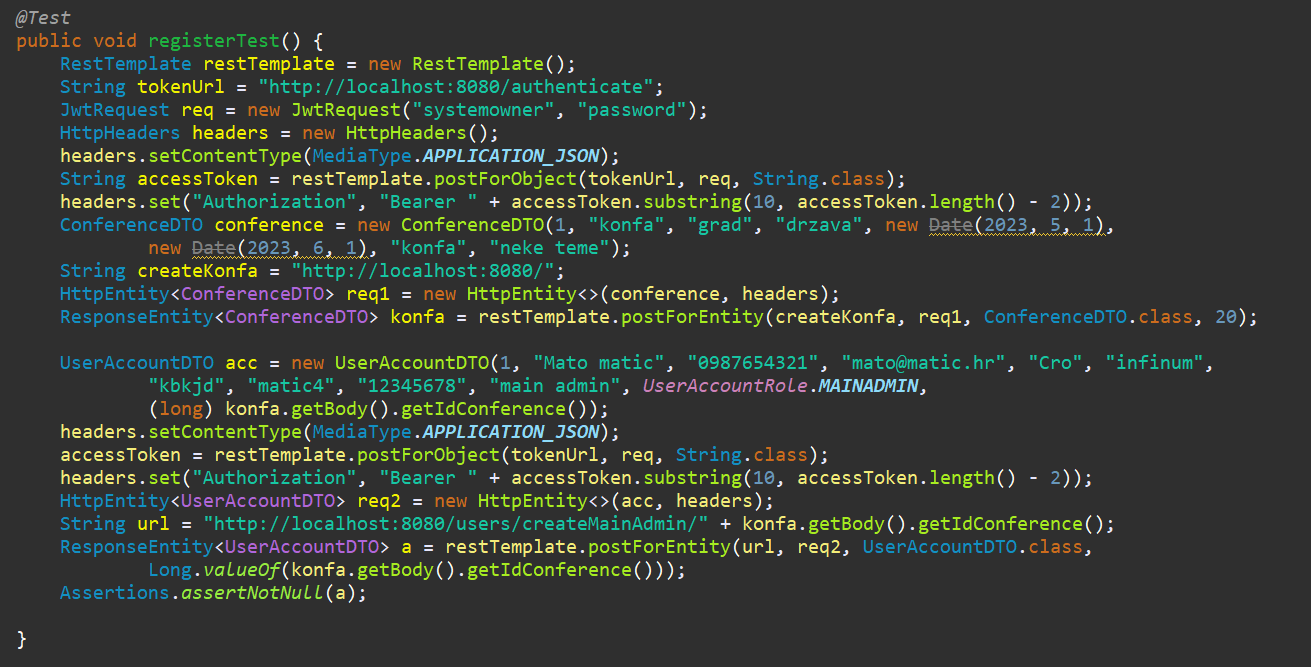
\includegraphics[scale=0.55]{slike/register_test.png} %veličina
			
			\centering
			\caption{Test ispravne registracije korisnika}
			\label{fig:ispravna registracija test}
			\end{figure}

    \begin{figure}[H]
            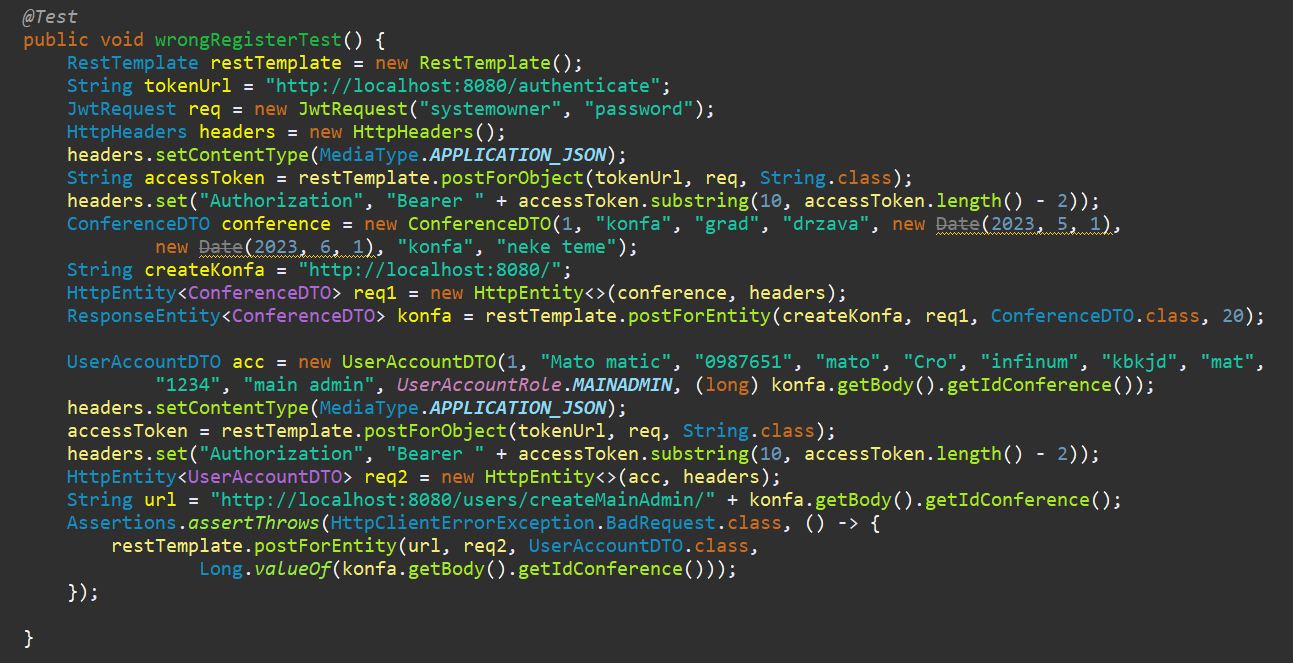
\includegraphics[scale=0.55]{slike/wrong_register_test.png} %veličina
			
			\centering
			\caption{Neispravna registracija korisnika}
			\label{fig:neispravna registracija korisnika}
			\end{figure}
  



   \textbf{\newline Ispitni slučaj 3: Kreiranje konferencije \newline}
   \textbf{Ulaz:}
   \begin{packed_item}
   \item[] \begin{packed_enum}
				
				\item Stvaranje konferencije sa svim ispravnim podatcima.
    \item Kreiranje konferencije s neispravnim podatcima (npr. datum početka je nakon datuma završetka).
				
			\end{packed_enum}
   \end{packed_item}

   \textbf{Očekivani rezultat:}
   \begin{packed_item}
   \item[] \begin{packed_enum}
				
				\item Kreiranje konferencije je uspješno. Kao odgovor se vraća kreirana konferencija.
    \item Kreiranje konferencije je neuspješno i kao odgovor se vraća BadRequest.
				
			\end{packed_enum}
   \end{packed_item}
   \textbf{Rezultat:} \text Svaki očekivani rezultat je ostvaren. \color{red} Aplikacija je prošla test. \color{black}

    \begin{figure}[H]
            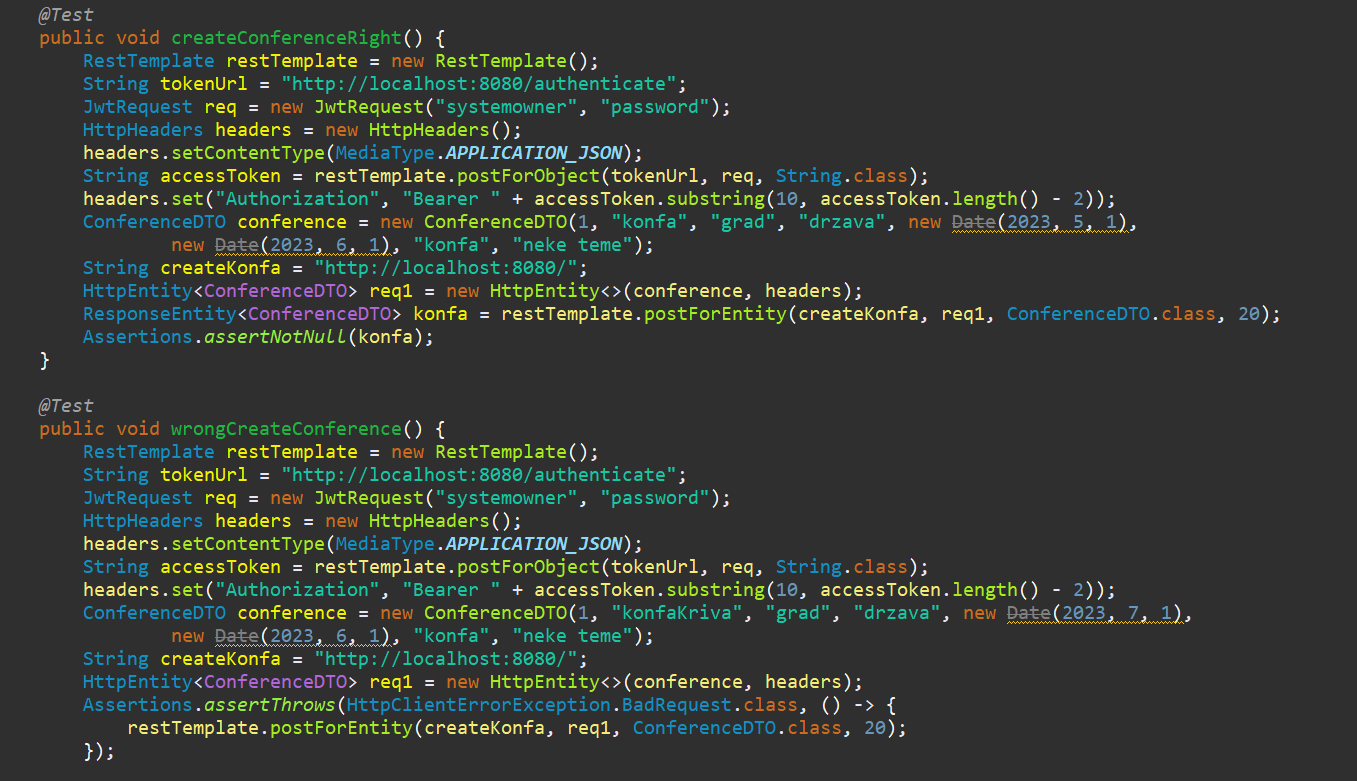
\includegraphics[scale=0.55]{slike/conf_test.png} %veličina
			
			\centering
			\caption{Testiranje kreiranja konferencije}
			\label{fig:test kreiranja konferencije}
			\end{figure}

   
   			\textbf{Ispitni slučaj 4: Stvaranje grupe podataka \newline}
   
   \textbf{Ulaz:}
   \begin{packed_item}
   \item[] \begin{packed_enum}
				
				\item Podatci o grupi podataka koju pokušava stvoriti ovlašteni glavni admin.
    \item Podatci o grupi podataka koju pokušava stvoriti neovlašteni operativni admin.
				
			\end{packed_enum}
   \end{packed_item}

   \textbf{Očekivani rezultat:}
   \begin{packed_item}
   \item[] \begin{packed_enum}
				
				\item Kreiranje grupe podataka je uspješno i kao odgovor se vraća stvorena grupa podataka.
    \item  Kreiranje grupe podataka je neuspješno i kao odgovor se vraća Forbidden.
				
			\end{packed_enum}
   \end{packed_item}
   \textbf{Rezultat:} \text Svaki očekivani rezultat je ostvaren. \color{red} Aplikacija je prošla test. \color{black}

    \begin{figure}[H]
            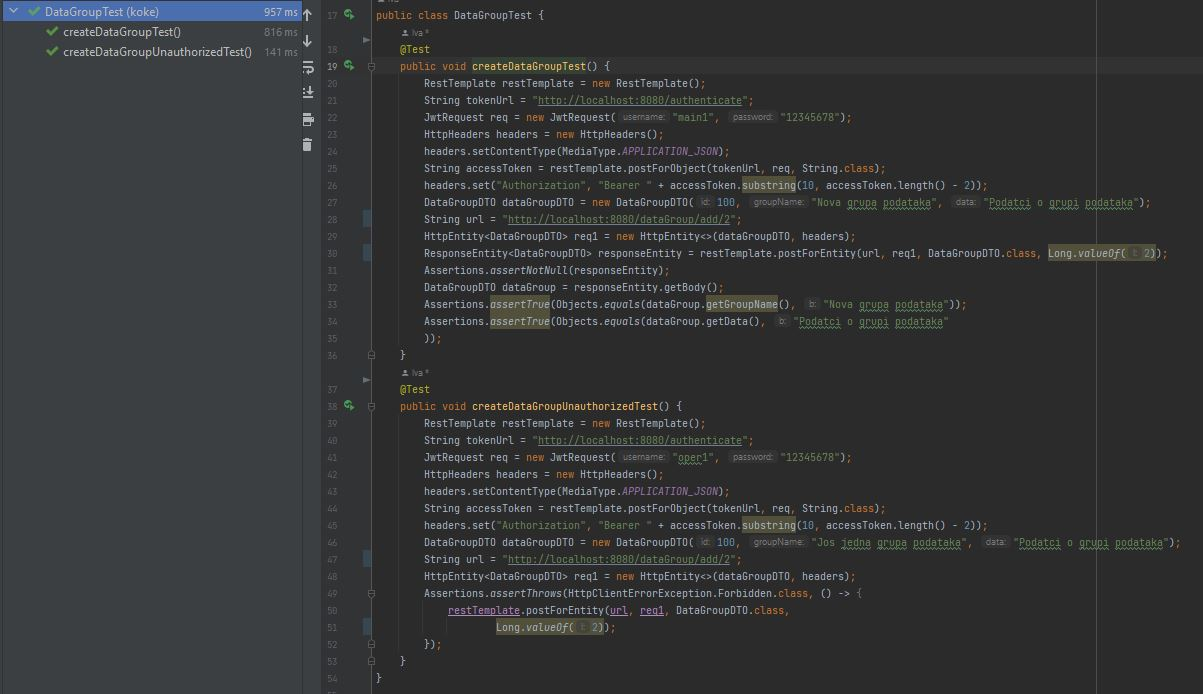
\includegraphics[scale=0.55]{slike/DataGroupTest.JPG} %veličina
			
			\centering
			\caption{Testiranje kreiranja grupe podataka}
			\label{fig:testiranje kreiranja grupe podataka}
			\end{figure}

   
   			\textbf{Ispitni slučaj 5: Stvaranje specijalnog događaja za konferenciju \newline}
   
   \textbf{Ulaz:}
   \begin{packed_item}
   \item[] \begin{packed_enum}
				
				\item Podatci o specijalnom događaju kojeg pokušava stvoriti ovlašteni glavni admin.
    \item Podatci o specijalnom događaju kojeg pokušava stvoriti neovlašteni operativni admin.
				
			\end{packed_enum}
   \end{packed_item}

   \textbf{Očekivani rezultat:}
   \begin{packed_item}
   \item[] \begin{packed_enum}
				
				\item Kreiranje specijalnog događaja je uspješno i kao odgovor se vraća stvoreni specijalni događaj.
    \item  Kreiranje specijalnog događaja je neuspješno i kao odgovor se vraća Forbidden.
				
			\end{packed_enum}
   \end{packed_item}
   \textbf{Rezultat:} \text Svaki očekivani rezultat je ostvaren. \color{red} Aplikacija je prošla test. \color{black}

    \begin{figure}[H]
            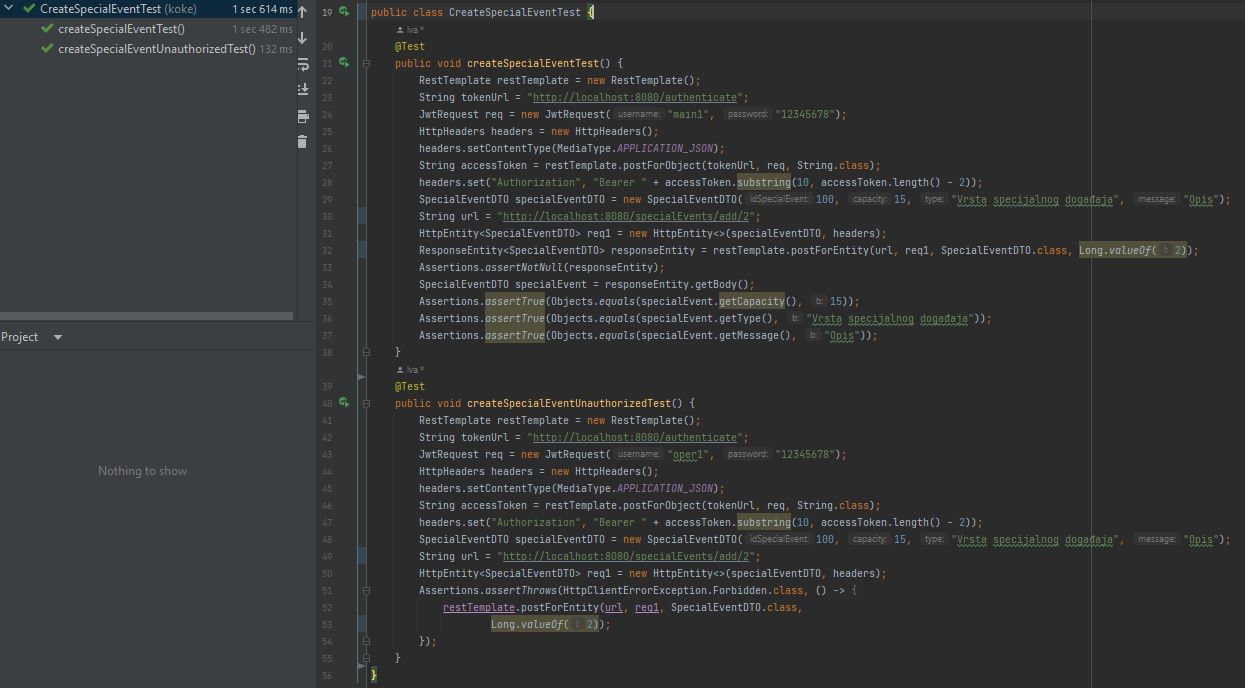
\includegraphics[scale=0.55]{slike/CreateSpecialEventTest.JPG} %veličina
			
			\centering
			\caption{Testiranje kreiranja specijalnog događaja}
			\label{fig:testiranje kreiranja specijalnog događaja}
			\end{figure}

   
   			\textbf{Ispitni slučaj 6: Prijava sudionika na specijalni događaj \newline}
   
   \textbf{Ulaz:}
   \begin{packed_item}
   \item[] \begin{packed_enum}
				
				\item Sudionik se prijavljuje na događaj kojem kapacitet nije popunjen.
    \item Sudionik se prijavljuje na događaj kojem kapacitet je popunjen.
				
			\end{packed_enum}
   \end{packed_item}

   \textbf{Očekivani rezultat:}
   \begin{packed_item}
   \item[] \begin{packed_enum}
				
				\item Sudionik se uspješno prijavio na događaj i kao odgovor se vraća taj  specijalni događaj.
    \item  Sudionik se nije prijavio na događaj, već je dodan u listu čekanja za taj događaj i na njegov email mu dolazi obavijest, a ovlaštenom glavnom adminu šalje se mail da lista čekanja nije prazna te da, ako je moguće, poveća kapacitet. Kao odgovor se vraća isti specijalni događaj.
				
			\end{packed_enum}
   \end{packed_item}
   \textbf{Rezultat:} \text Svaki očekivani rezultat je ostvaren. \color{red} Aplikacija je prošla test. \color{black}

    \begin{figure}[H]
            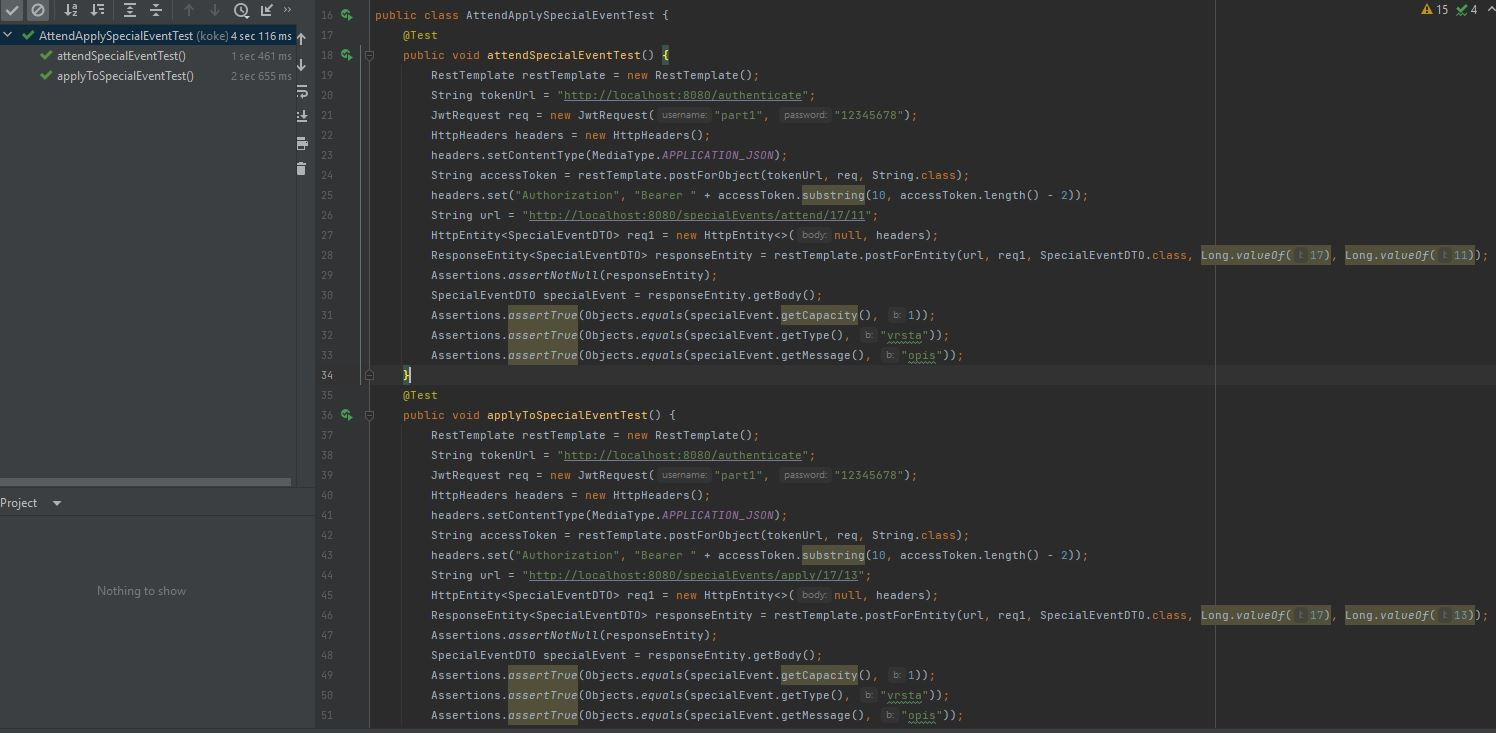
\includegraphics[scale=0.45]{slike/ApplyAttendSpecialEventTest.JPG} %veličina
			
			\centering
			\caption{Testiranje prijave na specijalni događaj}
			\label{fig:testiranje prijave na specijalni događaj}
			\end{figure}

   
   
   			\textbf{Ispitni slučaj 7: Povećanje kapaciteta specijalnog događaja \newline}
   
   \textbf{Ulaz:}
   \begin{packed_item}
   \item[] \begin{packed_enum}
				
				\item Ovlašteni glavni admin unosi za koliko želi povećati kapacitet specijalnog događaja.
				
			\end{packed_enum}
   \end{packed_item}

   \textbf{Očekivani rezultat:}
   \begin{packed_item}
   \item[] \begin{packed_enum}
				
				\item Kapacitet specijalnog događaja je povećan. Šalje se mail sudionicima na listi čekanja da su sada prijavljeni na specijalni događaj. Kao odgovor se vraća isti specijalni događaj.
				
			\end{packed_enum}
   \end{packed_item}
   \textbf{Rezultat:} \text Očekivani rezultat je ostvaren. \color{red} Aplikacija je prošla test. \color{black}

    \begin{figure}[H]
            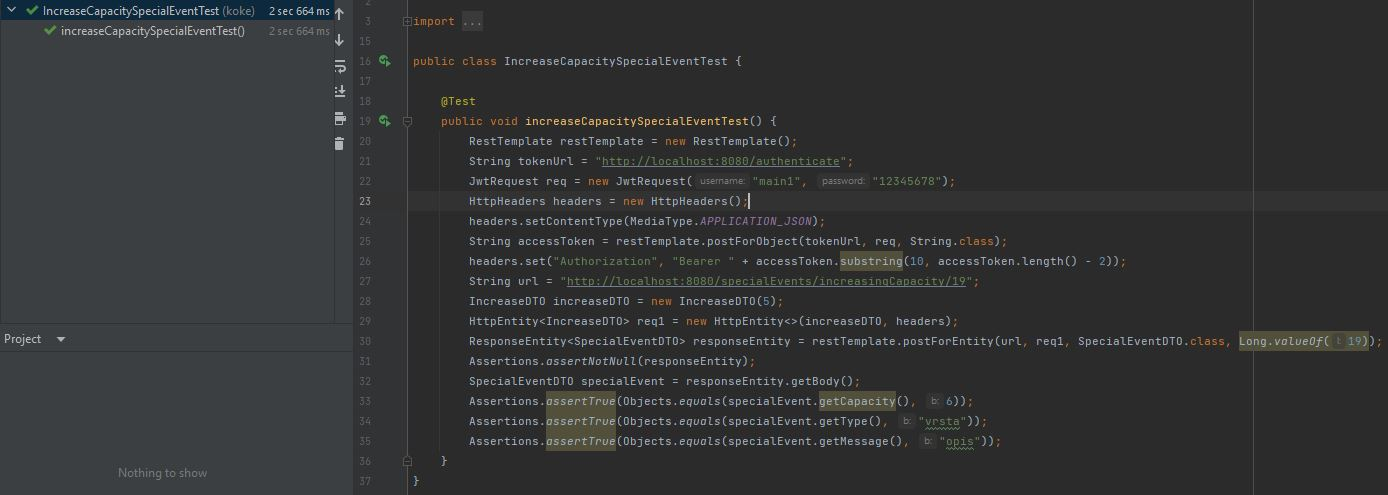
\includegraphics[scale=0.45]{slike/IncreaseCapacitySpecialEvent.JPG} %veličina
			
			\centering
			\caption{Testiranje povećanja kapaciteta specijalnog događaja}
			\label{fig:testiranje povećanja kapaciteta specijalnog događaja}
			\end{figure}

			
			\subsection{Ispitivanje sustava}
		\textbf{Ispitni slučaj 1: Uspješan login s postojećim korisnikom\newline}

  \newLine
   
   \textbf{Ulaz:}
   \begin{packed_item}
   \item[] \begin{packed_enum}
				
				\item Korisničko ime i lozinka postojećeg korisnika
				
			\end{packed_enum}
   \end{packed_item}

   \textbf{Očekivani rezultat:}
   \begin{packed_item}
   \item[] \begin{packed_enum}
				
				\item Login je uspješan i preusmjerava nas na početni izbornik. 
				
			\end{packed_enum}
   \end{packed_item}
   \textbf{Rezultat:} \text Očekivani rezultat je ostvaren. \color{red} Aplikacija je prošla test. \color{black}

    \begin{figure}[H]
            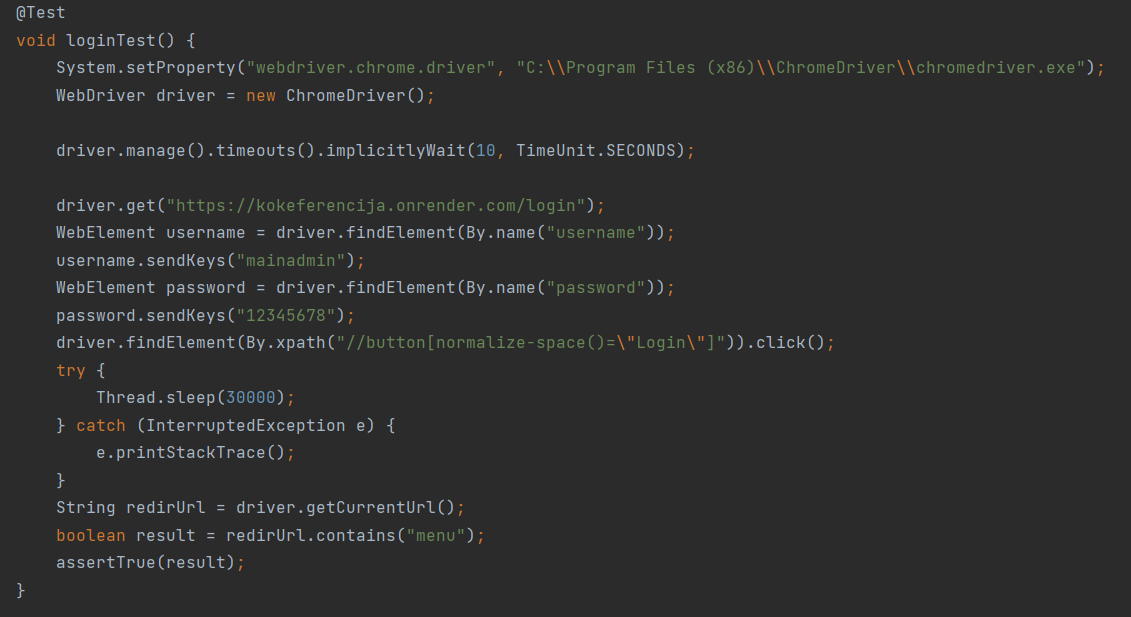
\includegraphics[width = \textwidth]{slike/Login succesful.png}
			
			\centering
			\caption{Uspješan login - Selenium}
			\label{fig:uspjesan login selenium}
			\end{figure}

   \textbf{Ispitni slučaj 2: Neuspješan login s nepostojećim korisnikom\newline}

  \newLine
   
   \textbf{Ulaz:}
   \begin{packed_item}
   \item[] \begin{packed_enum}
				
				\item Korisničko ime i lozinka nepostojećeg korisnika
				
			\end{packed_enum}
   \end{packed_item}

   \textbf{Očekivani rezultat:}
   \begin{packed_item}
   \item[] \begin{packed_enum}
				
				\item Login je neuspješan i ne preusmjerava nas na početni izbornik. 
				
			\end{packed_enum}
   \end{packed_item}
   \textbf{Rezultat:} \text Očekivani rezultat je ostvaren. \color{red} Aplikacija je prošla test. \color{black}

    \begin{figure}[H]
            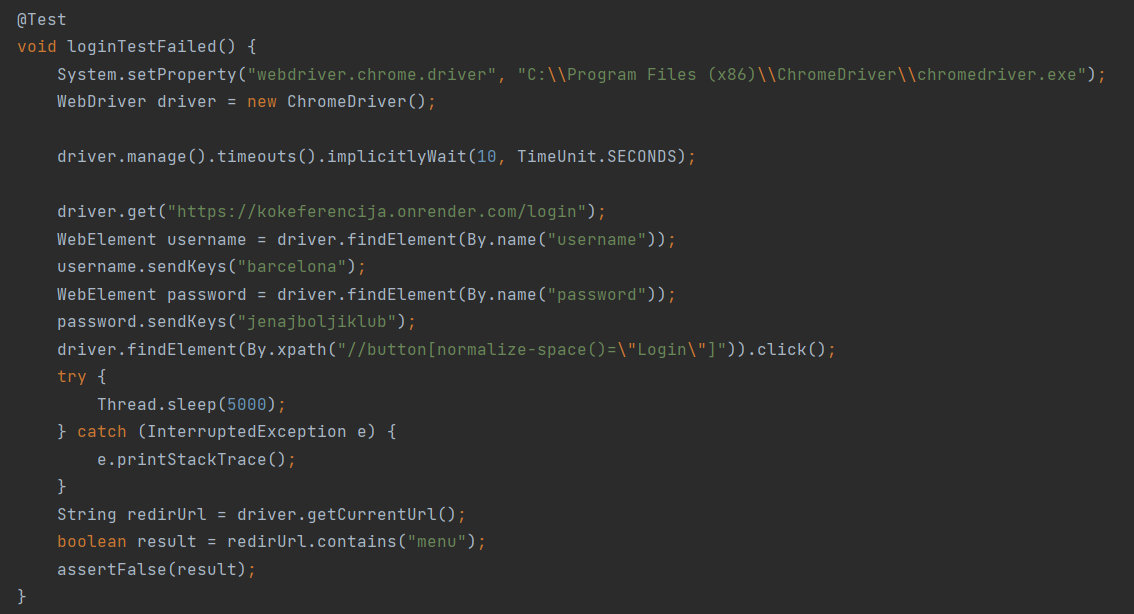
\includegraphics[width = \textwidth]{slike/login failed.png}
			
			\centering
			\caption{Neuspješan login - Selenium}
			\label{fig:neuspjesan login selenium}
			\end{figure}

   \eject

   \textbf{Ispitni slučaj 3: Otvaranje stranice MyConference\newline}

  \newLine
   
   \textbf{Ulaz:}
   \begin{packed_item}
            \item Korisničko ime i lozinka postojećeg korisnika
   \end{packed_item}

   \textbf{Očekivani rezultat:}
   \begin{packed_item}
   \item[] \begin{packed_enum}
				
				\item Uspješno se dohvaćaju svi resursi za prikaz stranice MyConference i stranica se uspješno prikazuje. 
				
			\end{packed_enum}
   \end{packed_item}
   \textbf{Rezultat:} \text Očekivani rezultat je ostvaren. \color{red} Aplikacija je prošla test. \color{black}

    \begin{figure}[H]
            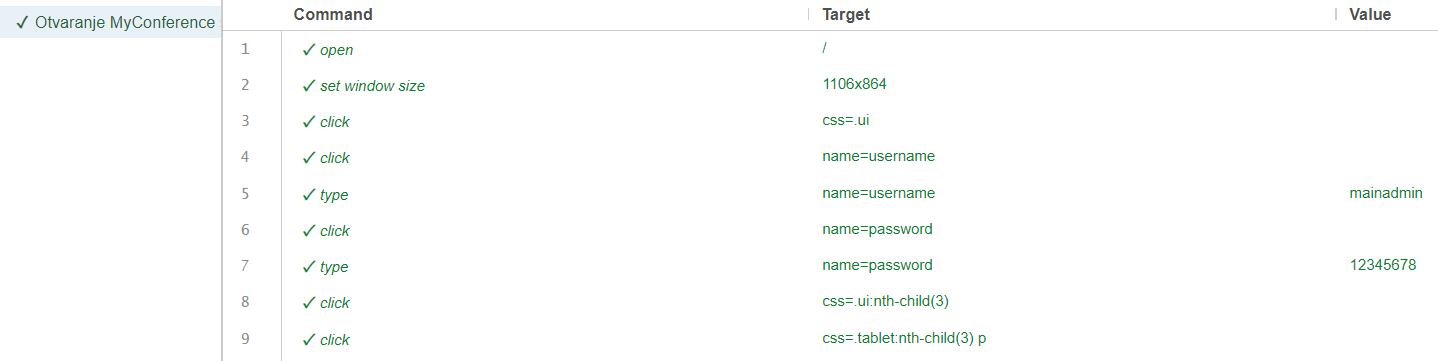
\includegraphics[width = \textwidth]{slike/MyConferenceTest.png}
			
			\centering
			\caption{Otvaranje MyConference test}
			\label{fig:myConferenceTest}
			\end{figure}

   \begin{figure}[H]
            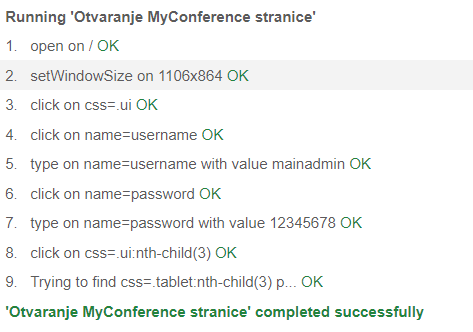
\includegraphics[scale = 0.8]{slike/MyConferenceRez.png}
			
			\centering
			\caption{Otvaranje MyConference rezultat}
			\label{fig:myConferenceRez}
			\end{figure}

   \textbf{Ispitni slučaj 4: Otvaranje galerije\newline}

  \newLine
   
   \textbf{Ulaz:}
   \begin{packed_item}
            \item Korisničko ime i lozinka postojećeg korisnika
   \end{packed_item}

   \textbf{Očekivani rezultat:}
   \begin{packed_item}
   \item[] \begin{packed_enum}
				
				\item Uspješno se dohvaćaju svi resursi za prikaz galerije i stranica se uspješno prikazuje. 
				
			\end{packed_enum}
   \end{packed_item}
   \textbf{Rezultat:} \text Očekivani rezultat je ostvaren. \color{red} Aplikacija je prošla test. \color{black}

    \begin{figure}[H]
            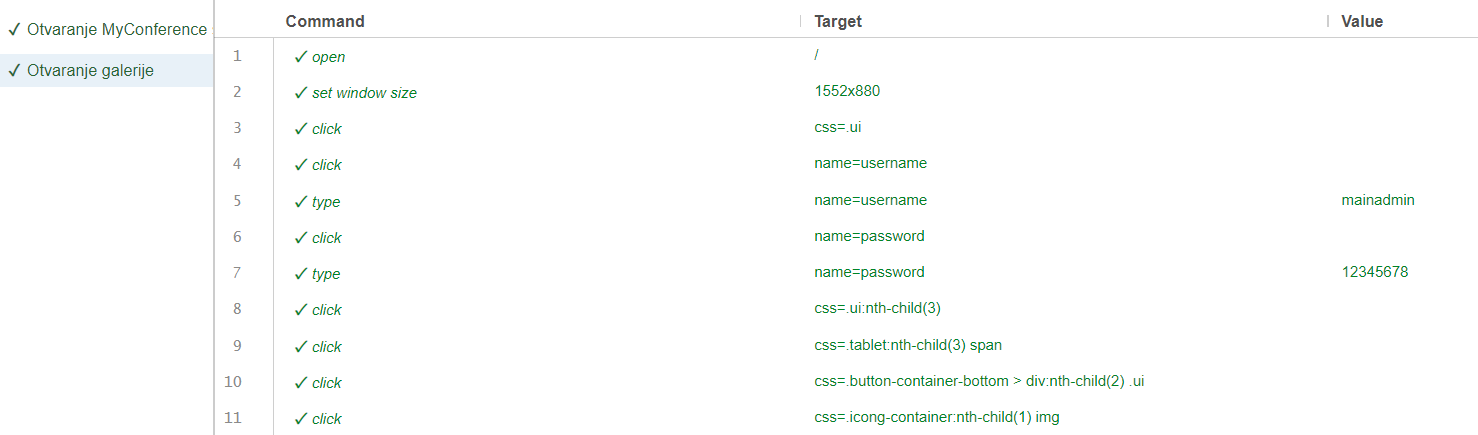
\includegraphics[width = \textwidth]{slike/OtvaranjeGalerije.png}
			
			\centering
			\caption{Otvaranje galerije test}
			\label{fig:myConferenceTest}
			\end{figure}

   \begin{figure}[H]
            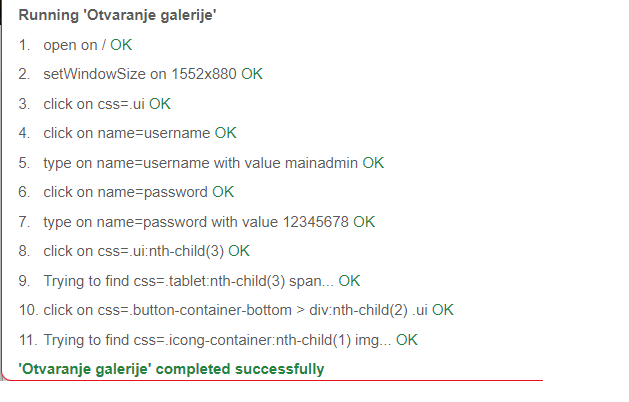
\includegraphics[scale = 0.8]{slike/OtvaranjeGalerijeRez.png}
			
			\centering
			\caption{Otvaranje galerije rezultat}
			\label{fig:myConferenceRez}
			\end{figure}
			
			\eject 
		
		
		\section{Dijagram razmještaja}
			
			Dijagram razmještaja opisuje topologiju sustava i usredotočen je na odnos
                sklopovskih i programskih dijelova. Arhitektura sustava aplikacije \textit{Kokeferencija} je ”klijent - poslužitelj” gdje se poslužitelj Render, na kojem se nalaze web stranica i baza podataka, nalazi na
                poslužiteljskom računalu, a klijenti koriste web preglednik kako bi pristupili web
                aplikaciji. Komunikacija između računala korisnika i poslužitelja odvija se preko 
                HTTP veze.

                \begin{figure}[H]
                 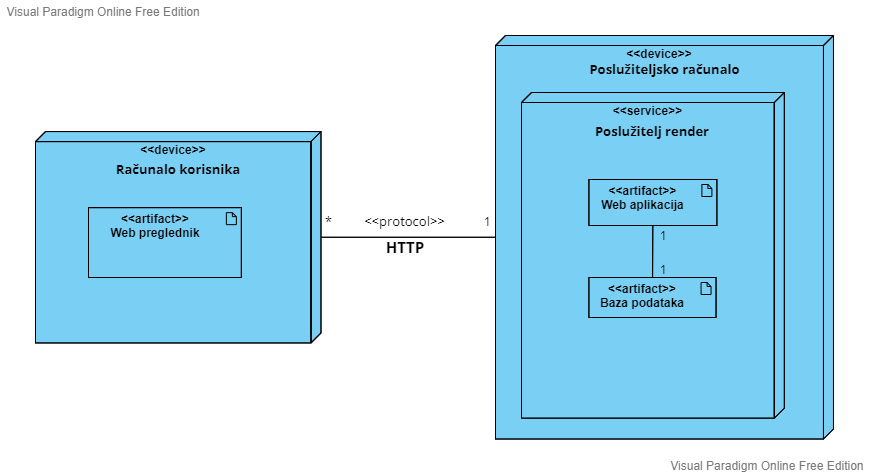
\includegraphics[scale = 0.55]{slike/dijagramRazmjestaja.png}
                \centering
                 \caption{dijagram razmještaja}
                 \label{fig:dijagram razmještaja}
                 \end{figure}\\

                 \eject


		
            \section{Upute za puštanje u pogon}

            \textbf{Postavljanje računa na Render\footnote{https://dashboard.render.com/}} \\
            Potrebno je stvoriti korisnički računa na Render-u, te 
           povezati ga s GitLab korisničkim računom kako bi mogli pristup projektu.\\
           \newLine

    \textbf{Konfiguracija i pokretanje poslužitelja baze podataka}\\
            Na nadzornoj ploči Rendera odabrati opciju New, zatim PostgreSQL. U polje \textit{Name} upisujemo ime baze koja se nalazi lokalno na našem računali, zatim u polja \textit{Database} i \textit{Username} opcionalno  upisujemo proizvoljno ime baze i korisničko ime. Za regiju odabiremo Frankfurt, te odgovarajuću PostegreSQL verziju. Za kraj odredimo besplatni plan. \\
            \newLine
             

            \textbf{Spajanje backend-a na poslužitelja baze podataka}\\
           U datoteku \textit{application.properties} upisujemo potrebne varijable. Kao \textit{spring.datasource.password} postavljamo lozinku koja se izgenerirala pri puštanju u pogon. Zatim postavljamo \textit{spring.datasource.username}. Url koji postavljamo ima oblik \textit{jdbc:postegreswl://hostname/database}. Za driver postavljamo \textit{org.postgresql.Driver}  Svi potrebi podatci o bazi koja je puštena u pogon nalaze se na Renderu(DashBoard 
            zatim naziv baze koji smo postavili pri pogonu). 
             U application.properties također dodamo liniju \textbf{server.servlet.context-path=/api} koja određuje prefiks svih zahtjeva na backend.
            \begin{figure}[H]
                 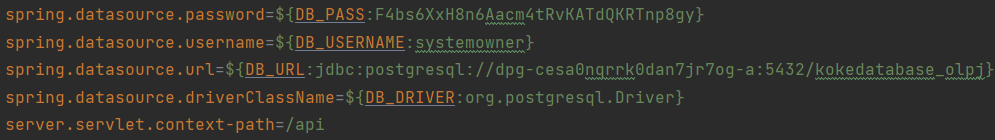
\includegraphics[width=\textwidth]{slike/application-properties.png}
                \centering
                 \caption{application.properties}
                 \label{fig:application.properties}
                 \end{figure}\\

        \textbf{Priprema backenda}\\
            Stvaramo Dockerfile u mapi u kojoj se nalazi \textit{sourcecode}. Konfiguracije datoteke jer prikazana na slici 5.10.
             \begin{figure}[H]
                 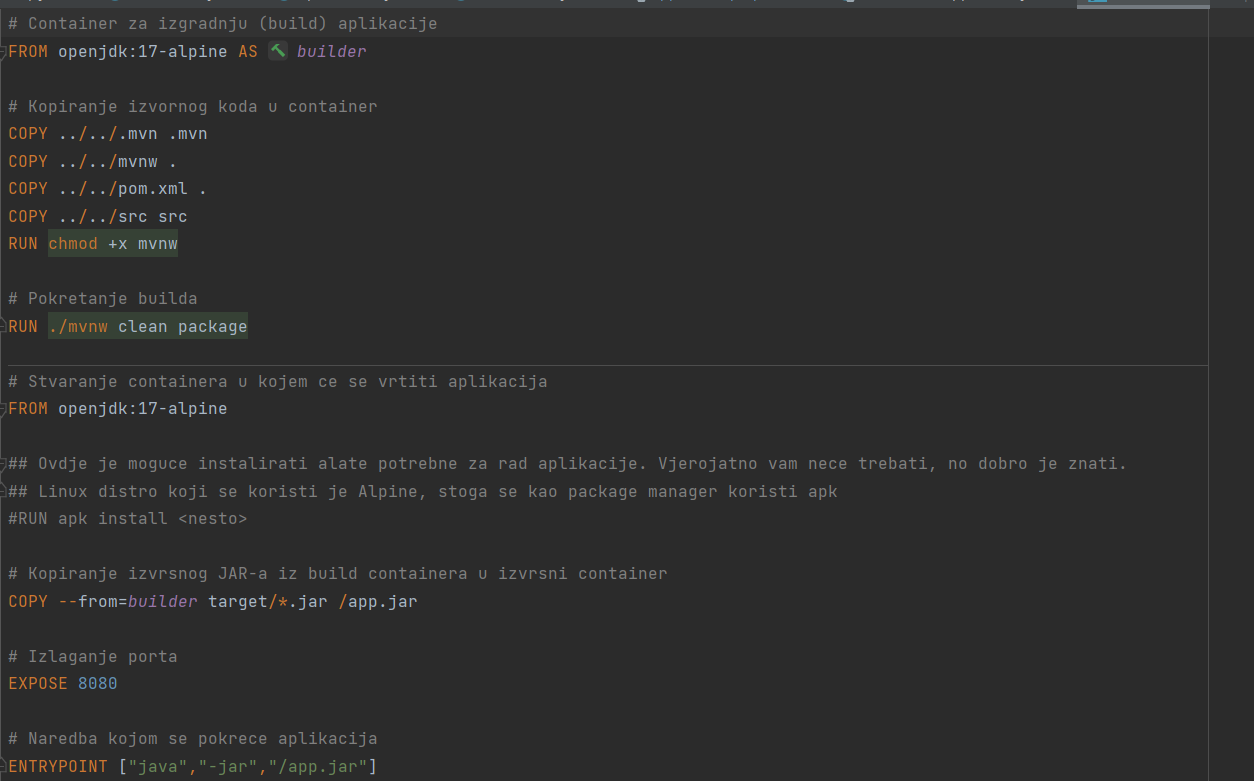
\includegraphics[scale = 0.5]{slike/Dockerfile.png}
                \centering
                 \caption{Dockerfile}
                 \label{fig:dockerfile}
                 \end{figure}\\\\

        \textbf{Puštanje backenda u pogon na Renderu}\\
            Na nadzornoj ploči Rendera izaberemo \textit{New} zatim \textit{Web Service}. Prikazat će se projekti povezanog GitLab računa. Pored odgovarajućeg projekta izaberemo \textit{Connect}. Postavljamo jedinstveno ime za servis (kokeferencije). Za regiju postavljamo Frankfurt. Zatim postavljamo granu na kojoj se nalazi kod i mapu u kojoj se nalazi izvorni kod. Za varijablu \textit{Environment} odabiremo \textit{Docker}.\\
            \begin{figure}[H]
                 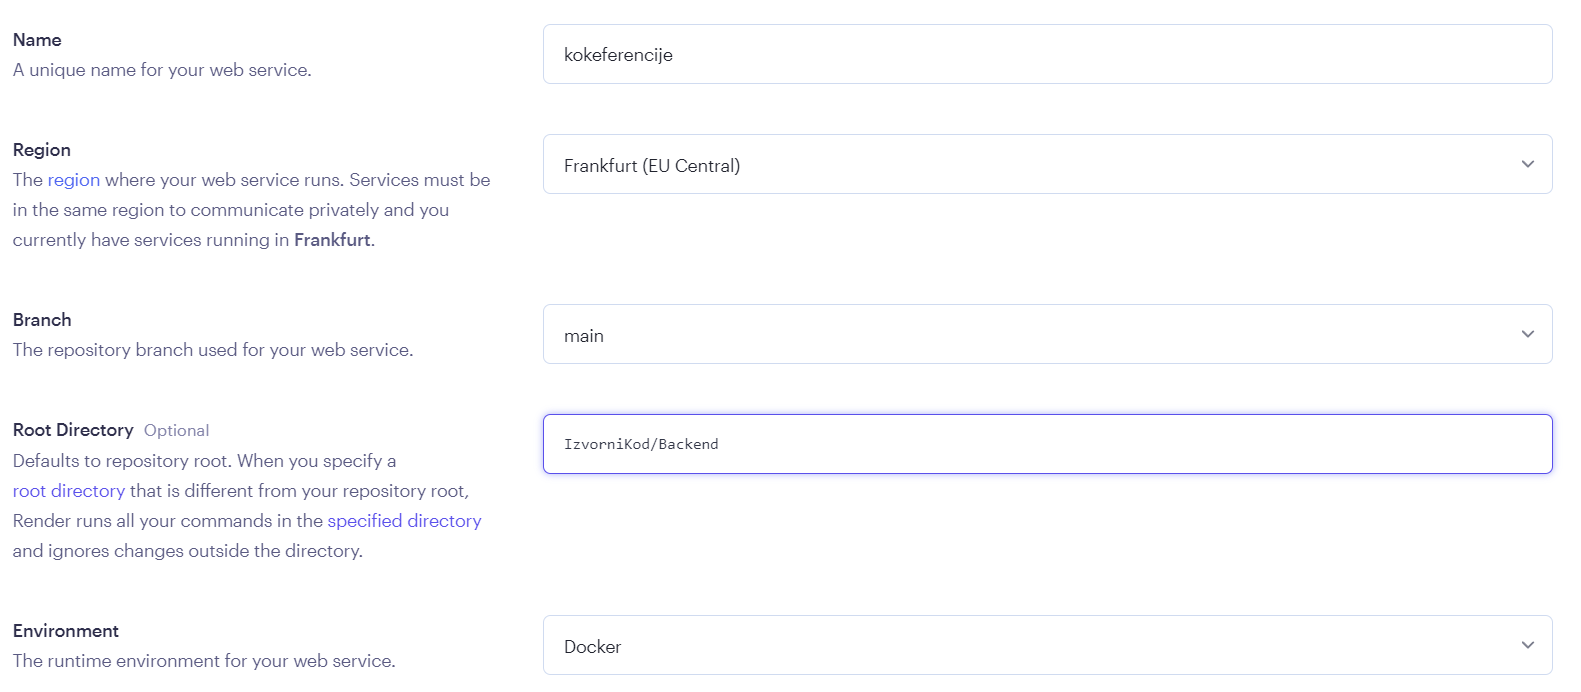
\includegraphics[width=\textwidth]{slike/Postavljanje backend za pogon.png}
                \centering
                 \caption{Postavljanje osnovnih varijabli za backend}
                 \label{fig:backend(1)}
                 \end{figure}
        Na dnu stranice odabiremo gumb \textit{Advanced}, zatim \textit{Add environment variable} te postavimo putanju za Dockerfile. Kada smo sve popunili odabiremo \textit{Create Web Service}.\\\\

        \textbf{Priprema frontenda}\\
        U package.json datoteku dodajemo ovisnosti potrebne za puštanje u pogon(http-proxy-middleware, dotenv, express)
         \begin{figure}[H]
                 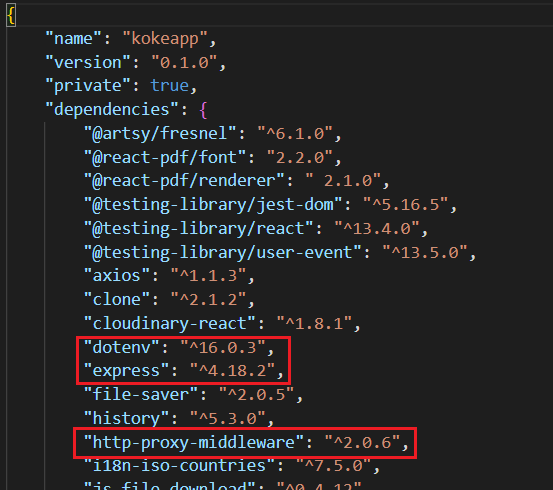
\includegraphics[scale = 0.70]{slike/package.json.png}
                \centering
                 \caption{package.json}
                 \label{fig:package.json}
                 \end{figure}
        U package.json izmijeniti naredbu \textbf{"build": "yarn install && react-scripts build"} i dodati naredbu \textbf{"start-prod": "node app.js"}.\\
        

        \textbf{Puštanje frontenda u pogon na Renderu}\\
             Na nadzornoj ploči Rendera izaberemo \textit{New} zatim \textit{Web Service}. Pored odgovarajućeg projekta odaberemo \textit{Connect}. Postavljamo ime za frontend servis koje će biti dio web-adrese (kokeferencija). Za regiju odabiremo Frankfurt, zatim odabiremo grane i mapu u kojoj se nalazi kod. Za varijablu \textit{Environment} biramo \textit{Node}. Za naredbu \textit{Build Command} postavljamo \textbf{yarn build}, a za \textit{Start Command} postavljamo \textbf{yarn start-prod}. Na dnu stranice odabiremo gumb \textit{Advanced} zatim \textit{Add Environment Variable}. Kao ključ postavljamo \textbf{APIBASEURL} a vrijednost postavljamo na adresu backend-a koji je pušten u pogon. Pritisnemo \textit{Create Web Service}. \\
        \textbf{Pokretanje web-stranice}\\
            Aplikaciji se može pristupiti preko adrese \textit{ https://kokeferencija.onrender.com/ \footnote{https://kokeferencija.onrender.com/}}.

    \eject 
	\chapter{Zaključak i budući rad}
				
		     Zadatak naše grupe bio je razvoj web aplikacije za konferencije. Omogućeno je prećenje dolaska sudionika na konferenciju, sudjelovanja sudionika u događanjima na konferenciji i davanje svih potrebnih informacija sudionicima. Rad na izradi aplikaciji trajao je 16 tjedana. Provedba projekta je bila kroz dvije faze.
   
             Prva faza projekta uključivala je okupljanje tima za razvoj aplikacije, dodjelu projektnog zadatka i dokumentiranje zahtjeva. Kvalitetna provedba prve faze uvelike je olakšala daljnji rad pri realizaciji osmišljenog sustava. Izrađeni obrasci i dijagrami (obrasci uporabe, sekvencijski dijagrami, model baze podataka, dijagram razreda) bili su od pomoći podtimovima zaduženima za razvoj \textit{backenda} i \textit{frontenda}. 
		
		     Dok se u prvoj fazi najvećim dijelom fokusiralo na grupnom pronalaženju optimalnog rješenja, druga faza projekta bila je puno intenzivnija po pitanju samostalnog rada članova. Članovi tima bili su bez iskustva rada na sličnim projektima te su dosta vremena potrošili na upoznavanje i učenje odabranih alata za izradu aplikacije. Također puno vremena potrošeno je na puštanje aplikacije u pogon. Osim realizacije rješenja i \textit{deploy}-a, u drugoj fazi je bilo potrebno dokumentirati ostale UML dijagrame i izraditi popratnu dokumentaciju kako bi budući korisnici mogli lakše koristiti. Dokumentiranje iz prve faze uštedjelo nam je na vremenu tijekom konkretne izrade aplikacije, iako je bilo manjih izmjena i dorada kako se aplikacija razvijala.

             Komunikacija između članova tima bila je većinom putem WhatsAppa, a manjim dijelom i Discorda. Moguće proširenje projekta bila bi izrada mobile aplikacije za lakše i efikasnije korištenje stalnim korisnicima.

             Rad na ovom projektu bilo je jako vrijedno te ujedno i novo iskustvo članovima tima. Naučili smo puno o radu u timu te smo proširili znanje u smislu poznavanja novih alata. Svjesni smo da aplikacija ima puno prostora za poboljšanje, no iznimno smo zadovoljni postignutim rezultatom projekta upravo zbog neiskustva svih članova tima.
		
		\eject 
	\chapter*{Popis literature}
		\addcontentsline{toc}{chapter}{Popis literature}
		
		
		\begin{enumerate}
			
			
			\item  Programsko inženjerstvo, FER ZEMRIS, \url{http://www.fer.hr/predmet/proinz}
			
			\item Stack Overflow,
			\url{https://stackoverflow.com/}
			
			\item  Geeks for Geeks,
			\url{https://www.geeksforgeeks.org/}
			
			\item  W3 Schools,
			\url{https://www.w3schools.com/}
			
			\item  The Unified Modeling Language, \url{https://www.uml-diagrams.org/}
			
			\item  Javatpoint, \url{https://www.javatpoint.com/}
			
			\item  Astah Community, \url{http://astah.net/editions/uml-new}
			\item Visual Paradigm, \url{https://www.visual-paradigm.com/}
		\end{enumerate}
		
		 
	
	
	\begingroup
	\renewcommand*\listfigurename{Indeks slika i dijagrama}
	%\renewcommand*\listtablename{Indeks tablica}
	%\let\clearpage\relax
	\listoffigures
	%\vspace{10mm}
	%\listoftables
	\endgroup
	\addcontentsline{toc}{chapter}{Indeks slika i dijagrama}


	
	\eject 
		
	\chapter*{Dodatak: Prikaz aktivnosti grupe}
		\addcontentsline{toc}{chapter}{Dodatak: Prikaz aktivnosti grupe}
		
		\section*{Dnevnik sastajanja}
		
		\begin{packed_enum}
			\item  sastanak
			
			\item[] \begin{packed_item}
				\item Datum: 20. listopada 2022.
				\item Prisustvovali: N.Benić, J.Markić, A.Ćepić, D.Dragojević, A.Kaselj, I.Ursić, V.Valić
				\item Teme sastanka:
				\begin{packed_item}
					\item  sastanak s asistentom i demonstratorom
					\item  upute i analiza zadatka
				\end{packed_item}
			\end{packed_item}
			
			\item  sastanak
			\item[] \begin{packed_item}
				\item Datum: 24. listopada 2022.
				\item Prisustvovali: N.Benić, J.Markić, A.Ćepić, D.Dragojević, A.Kaselj, I.Ursić, V.Valić
				\item Teme sastanka:
				\begin{packed_item}
					\item  dogovor odabira alata i tehnologija
					\item  pravljenje kanban ploče na gitu
					\item  izrada osnovnog plana po tjednima
				\end{packed_item}
			\end{packed_item}
		
			\item  sastanak
			\item[] \begin{packed_item}
				\item Datum: 25. listopada 2022.
				\item Prisustvovali: N.Benić, J.Markić, A.Ćepić, D.Dragojević, A.Kaselj, I.Ursić, V.Valić
				\item Teme sastanka:
				\begin{packed_item}
					\item  razrada inicijalnog ER modela
					\item  diskusija funkcionalnosti
					\item  podjela poslova na relacijski model i obrasce uporabe
				\end{packed_item}
			\end{packed_item}
		
			\item  sastanak
			\item[] \begin{packed_item}
				\item Datum: 27. listopada 2022.
				\item Prisustvovali: N.Benić, D.Dragojević, A.Kaselj, I.Ursić
				\item Teme sastanka:
				\begin{packed_item}
					\item  sastanak s asistentom i demonstratorom - diskusija dosadašnjeg rada
					\item  konačan odabir alata i tehnologija
					\item  raščišćavanje dilema o funkcionalnostima
				\end{packed_item}
			\end{packed_item}
		
			\item  sastanak
			\item[] \begin{packed_item}
				\item Datum: 31. listopada 2022.
				\item Prisustvovali: N.Benić, J.Markić, A.Ćepić, D.Dragojević, A.Kaselj, I.Ursić, V.Valić
				\item Teme sastanka:
				\begin{packed_item}
					\item  podjela poslova za izradu baze i backenda
					\item  dogovor za pisanje dokumentacije
				\end{packed_item}
			\end{packed_item}

                \item  sastanak
			\item[] \begin{packed_item}
				\item Datum: 2. studenog 2022.
				\item Prisustvovali: N.Benić, A.Ćepić, A.Kaselj, I.Ursić
				\item Teme sastanka:
				\begin{packed_item}
					\item  pregled backenda
					\item  popis klasa i metoda
				\end{packed_item}
			\end{packed_item}

                \item  sastanak
			\item[] \begin{packed_item}
				\item Datum: 3. studenog 2022.
				\item Prisustvovali: N.Benić, I.Ursić
				\item Teme sastanka:
				\begin{packed_item}
					\item  sastanak s asistentom i demonstratorom- diskusija dosadašnjeg rada
					\item  razrada vrsta korisnika
                        \item ispravke u bazi
				\end{packed_item}
			\end{packed_item}

                \item  sastanak
			\item[] \begin{packed_item}
				\item Datum: 8. studenog 2022.
				\item Prisustvovali: N.Benić, I.Ursić, A.Ćepić, D.Dragojević, J.Markić, V.Valić, A.Kaselj 
				\item Teme sastanka:
				\begin{packed_item}
					\item podjela ostatka posla
					\item  dogovor oko daljnje implementacije
				\end{packed_item}
			\end{packed_item}

                \eject

                \item  sastanak
			\item[] \begin{packed_item}
				\item Datum: 15. studenog 2022.
				\item Prisustvovali: N.Benić, I.Ursić, A.Ćepić, D.Dragojević, J.Markić, V.Valić, A.Kaselj 
				\item Teme sastanka:
				\begin{packed_item}
					\item čiščenje gita, rad na deploymentu aplikacije
					\item  završavanje dokumentacije
				\end{packed_item}
			\end{packed_item}

    \item  sastanak
			\item[] \begin{packed_item}
				\item Datum: 6. prosinca 2022.
				\item Prisustvovali: N.Benić, I.Ursić, A.Ćepić, D.Dragojević, J.Markić, V.Valić, A.Kaselj 
				\item Teme sastanka:
				\begin{packed_item}
					\item Dokumentacija
					\item  određivanje novih zadataka
				\end{packed_item}
			\end{packed_item}

   \item  sastanak
			\item[] \begin{packed_item}
				\item Datum: 7. prosinca 2022.
				\item Prisustvovali:  I.Ursić, D.Dragojević, J.Markić, A.Kaselj 
				\item Teme sastanka:
				\begin{packed_item}
					\item  određivanje novih zadataka za backend
				\end{packed_item}
			\end{packed_item}

   \item  sastanak
			\item[] \begin{packed_item}
				\item Datum: 8. prosinca 2022.
				\item Prisustvovali: N.Benić, I.Ursić, A.Ćepić, D.Dragojević, J.Markić, V.Valić, A.Kaselj 
				\item Teme sastanka:
				\begin{packed_item}
					\item  određivanje novih zadataka za frontend i backend
				\end{packed_item}
			\end{packed_item}

   \item  sastanak
			\item[] \begin{packed_item}
				\item Datum: 9. prosinca 2022.
				\item Prisustvovali: N.Benić, I.Ursić, A.Ćepić, D.Dragojević, J.Markić, V.Valić, A.Kaselj 
				\item Teme sastanka:
				\begin{packed_item}
					\item  određivanje novih zadataka za frontend i backend
				\end{packed_item}
			\end{packed_item}

   \eject

   \item  sastanak
			\item[] \begin{packed_item}
				\item Datum: 2. siječnja 2023.
				\item Prisustvovali: N.Benić, I.Ursić, A.Ćepić, D.Dragojević, J.Markić, V.Valić, A.Kaselj 
				\item Teme sastanka:
				\begin{packed_item}
					\item  dogovor o pisanju dokumentacije
				\end{packed_item}
			\end{packed_item}

    \item  sastanak
			\item[] \begin{packed_item}
				\item Datum: 11. siječnja 2023.
				\item Prisustvovali: N.Benić, I.Ursić, A.Ćepić, D.Dragojević, J.Markić, V.Valić 
				\item Teme sastanka:
				\begin{packed_item}
					\item  ispravak i provjera dokumentacije
				\end{packed_item}
			\end{packed_item}
			
			%
			
		\end{packed_enum}
		
		\eject
		\section*{Tablica aktivnosti}

			\begin{longtblr}[
					label=none,
				]{
					vlines,hlines,
					width = \textwidth,
					colspec={X[7, l]X[1, c]X[1, c]X[1, c]X[1, c]X[1, c]X[1, c]X[1, c]}, 
					vline{1} = {1}{text=\clap{}},
					hline{1} = {1}{text=\clap{}},
					rowhead = 1,
				} 
				\multicolumn{1}{c|}{} & \multicolumn{1}{c|}{\rotatebox{90}{\textbf{Nikoleta Benić}}} & \multicolumn{1}{c|}{\rotatebox{90}{\textbf{Josipa Markić }}} &	\multicolumn{1}{c|}{\rotatebox{90}{\textbf{Iva Ursić }}} & \multicolumn{1}{c|}{\rotatebox{90}{\textbf{Valentina Valić }}} &	\multicolumn{1}{c|}{\rotatebox{90}{\textbf{Ana Ćepić }}} & \multicolumn{1}{c|}{\rotatebox{90}{\textbf{Andrea Kaselj }}} &	\multicolumn{1}{c|}{\rotatebox{90}{\textbf{Dorotea Dragojević }}} \\  
				Upravljanje projektom 		&6  &6  &6  &6  &10  &8  &10 \\ 
				Opis projektnog zadatka 	&0  &0  &0  &4  &0  &0  &0 \\ 
				
				Funkcionalni zahtjevi       &0  &0  &0  &0  &3  &0  &0  \\ 
				Opis pojedinih obrazaca 	&4  &0  &4  &0  &2  &0  &0  \\ 
				Dijagram obrazaca 			&0  &0  &1.5  &0  &2  &3  &0  \\ 
				Sekvencijski dijagrami 		&0  &1.5  &0  &0  &4  &0  &0  \\ 
				Opis ostalih zahtjeva 		&0  &0  &0.5  &0  &0  &1  &0  \\ 

				Arhitektura i dizajn sustava	 &0  &0  &0  &0  &0  &4  &0  \\ 
				Baza podataka				&0  &5.5  &0  &0  &0  &0  &0.5   \\ 
				Dijagram razreda 			&5  &0  &0  &0  &0  &0  &0   \\ 
				Dijagram stanja				&1.5  &0  &0  &0  &0  &0  &0  \\ 
				Dijagram aktivnosti 		&0  &0  &0  &0  &0  &0  &3  \\ 
				Dijagram komponenti			&0  &0  &0  &0  &1  &0  &0  \\ 
				Korištene tehnologije i alati 		&0  &0  &0  &1  &0  &0  &0  \\ 
				Ispitivanje programskog rješenja 	&1  &0  &1  &0  &0  &0  &0.75  \\ 
				Dijagram razmještaja			&0  &1.5  &0  &0  &0  &0  &0  \\ 
				Upute za puštanje u pogon 		&1 &0  &0  &0  &0  &0  &0  \\  
				Dnevnik sastajanja 			&0  &0  &0  &0  &0  &1  &2  \\ 
				Zaključak i budući rad 		&0  &0  &1  &0  &0  &0  &0  \\  
				Popis literature 			&0  &0  &0  &0.2  &0  &0  &0  \\   \hline 
				Frontend 				&40  &20  &0  &38  &55  &0  &0  \\  
				Izrada baze podataka	 			&3  &8  &3  &8  &3  &3  &13 \\  
				Spajanje s bazom podataka						&2  &0  &2  &4  &0  &0  &2  \\ 
				Backend 							&15 &45  &55 &20  &25  &0  &51.5  \\  
                Puštanje aplikacije u pogon						&2  &20  &22  &4  &11  &5  &14  \\  
                Testiranje						&0  &0  &3  &0  &3  &0  &5  \\ 
			\end{longtblr}
					
					
		\eject
		\section*{Dijagrami pregleda promjena}
		
		
		 \begin{figure}[H]
            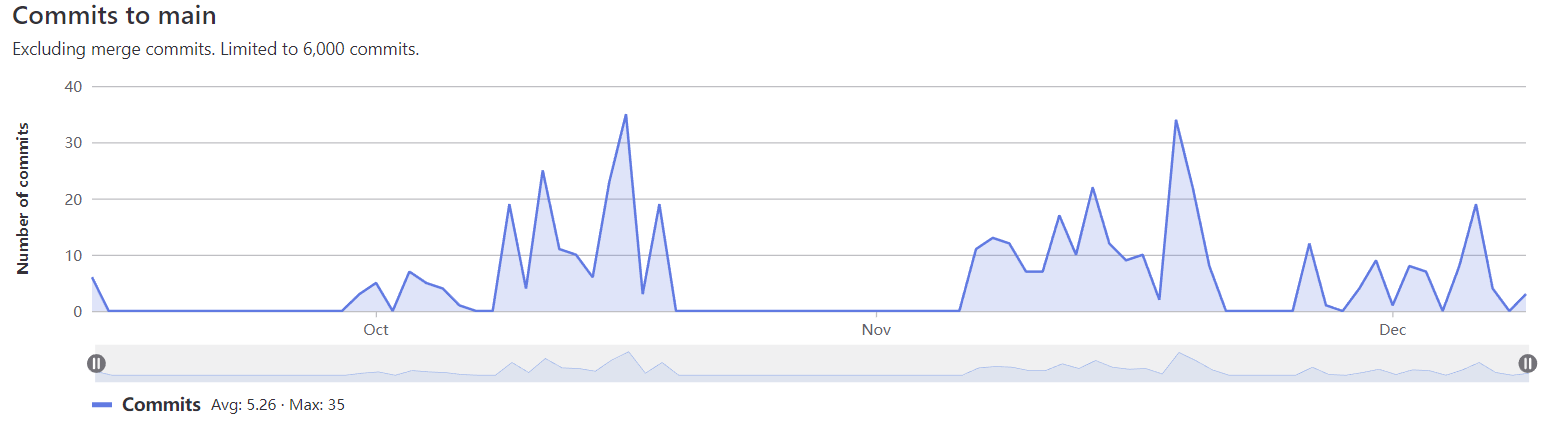
\includegraphics[scale=0.50]{slike/commits_main.png} %veličina
			
			\centering
			\caption{Commitovi na main grani}
			\label{fig:Commitovi na main grani}
			\end{figure}

         \begin{figure}[H]
            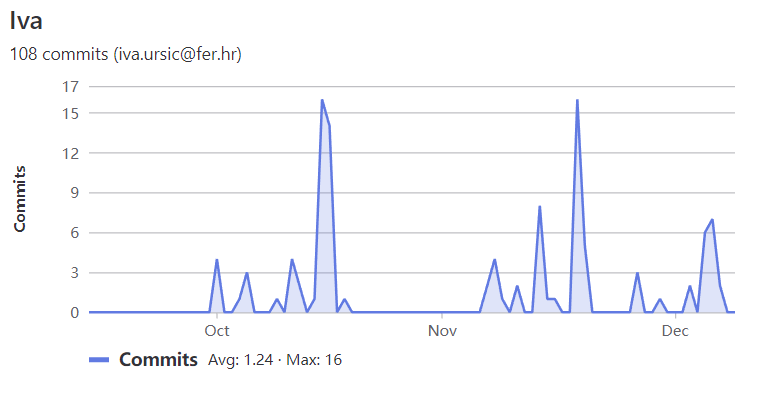
\includegraphics[scale=1]{slike/commits_iva_ursic.png} %veličina
			
			\centering
			\caption{Iva Ursić - commits}
			\label{fig:Iva Ursić commits}
			\end{figure}
         \begin{figure}[H]
            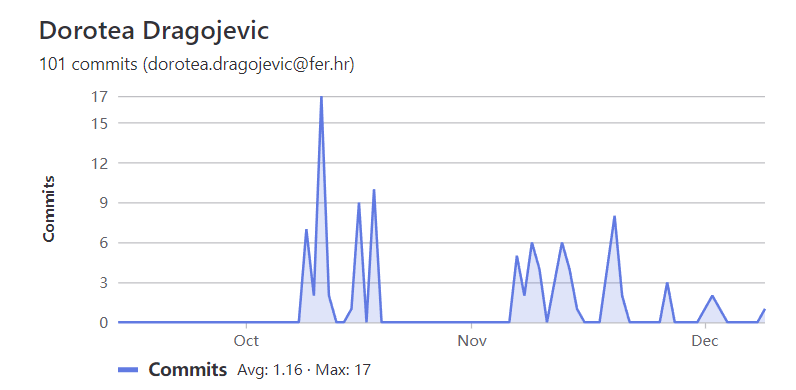
\includegraphics[scale=1]{slike/commits_dorotea_dragojevic.png} %veličina
			
			\centering
			\caption{Dorotea Dragojević - commits}
			\label{fig:Dorotea Dragojević - commits}
			\end{figure}
         \begin{figure}[H]
            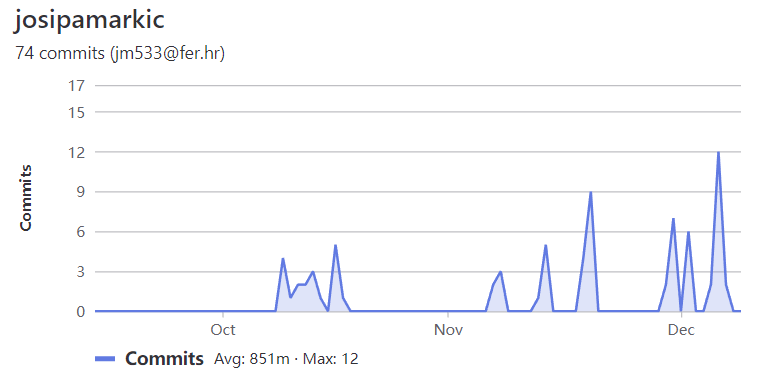
\includegraphics[scale=1]{slike/commits_josipa_markic.png} %veličina
			
			\centering
			\caption{Josipa Markić - commits}
			\label{fig:Josipa Markić commits}
			\end{figure}
    \begin{figure}[H]
            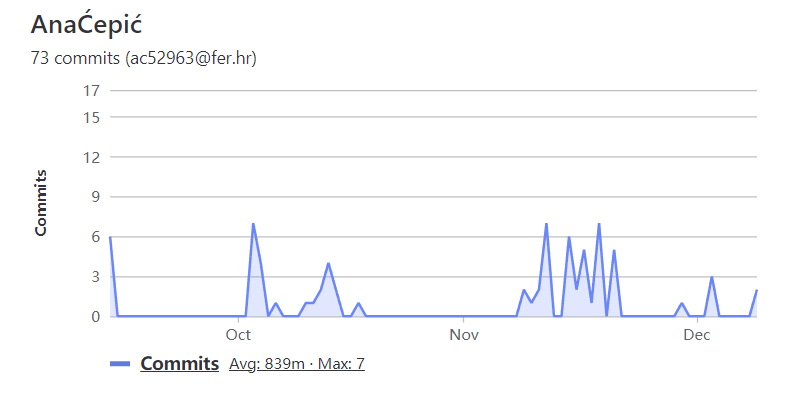
\includegraphics[scale=1]{slike/commits_ana_cepic.png} %veličina
			
			\centering
			\caption{Ana Ćepić - commits}
			\label{fig:Ana Ćepić commits}
			\end{figure}

    \begin{figure}[H]
            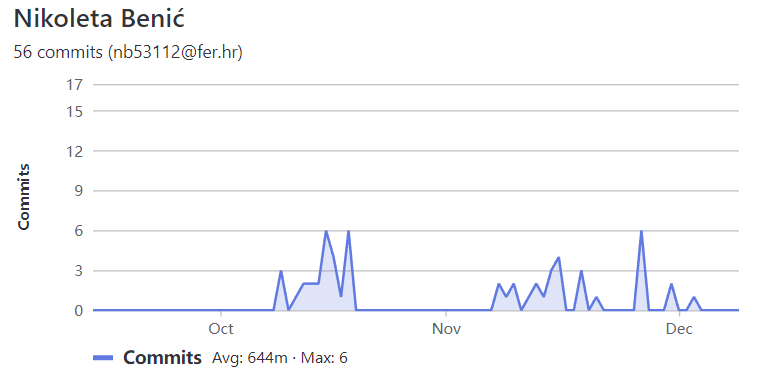
\includegraphics[scale=1]{slike/commits_nikoleta_benic.png} %veličina
			
			\centering
			\caption{Nikoleta Benić - commits}
			\label{fig:Nikoleta Benić commits}
			\end{figure}

    \begin{figure}[H]
            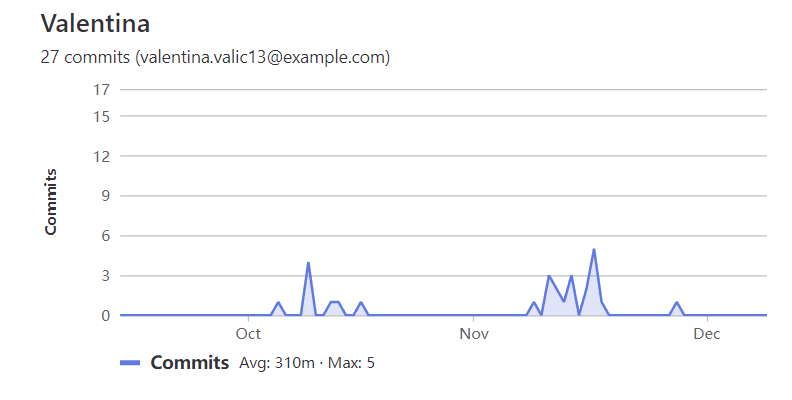
\includegraphics[scale=1]{slike/commits_valentina_valic.png} %veličina
			
			\centering
			\caption{Valentina Valić - commits}
			\label{fig:Valentina Valić commits}
			\end{figure}

    \begin{figure}[H]
            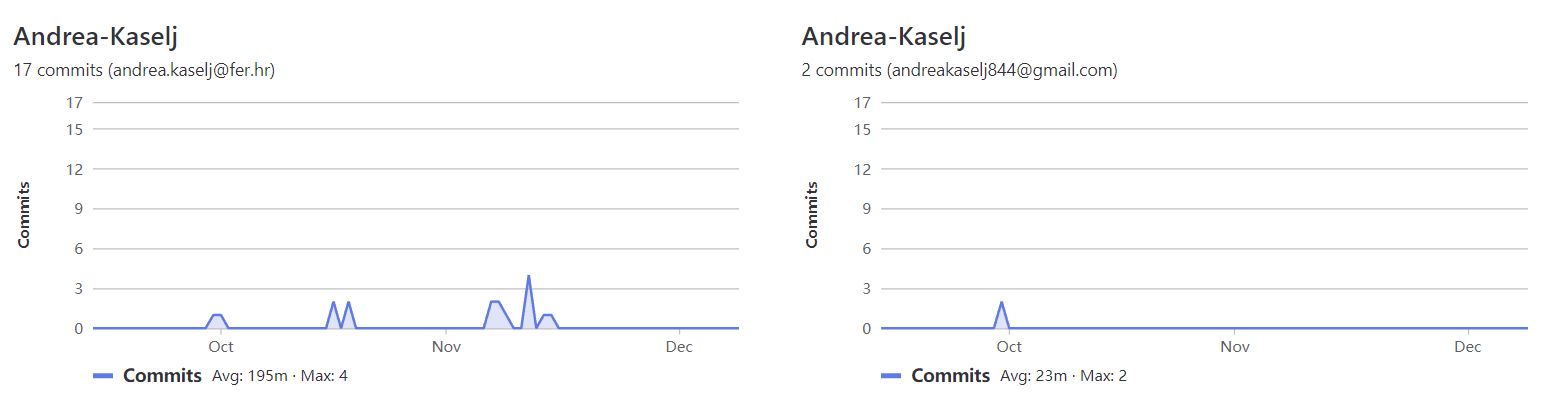
\includegraphics[scale=0.50]{slike/commits_andrea_kaselj.png} %veličina
			
			\centering
			\caption{Andrea Kaselj - commits}
			\label{fig:Andrea Kaselj commits}
			\end{figure}
   
		
	

		
	
			\chapter*{Dodatak: Prikaz aktivnosti grupe}
			\addcontentsline{toc}{chapter}{Dodatak: Prikaz aktivnosti grupe}
			
			\section*{Dnevnik sastajanja}
			
			\begin{packed_enum}
				\item  sastanak
				
				\item[] \begin{packed_item}
					\item Datum: 20. listopada 2022.
					\item Prisustvovali: N.Benić, J.Markić, A.Ćepić, D.Dragojević, A.Kaselj, I.Ursić, V.Valić
					\item Teme sastanka:
					\begin{packed_item}
						\item  sastanak s asistentom i demonstratorom
						\item  upute i analiza zadatka
					\end{packed_item}
				\end{packed_item}
				
				\item  sastanak
				\item[] \begin{packed_item}
					\item Datum: 24. listopada 2022.
					\item Prisustvovali: N.Benić, J.Markić, A.Ćepić, D.Dragojević, A.Kaselj, I.Ursić, V.Valić
					\item Teme sastanka:
					\begin{packed_item}
						\item  dogovor odabira alata i tehnologija
						\item  pravljenje kanban ploče na gitu
						\item  izrada osnovnog plana po tjednima
					\end{packed_item}
				\end{packed_item}
			
				\item  sastanak
				\item[] \begin{packed_item}
					\item Datum: 25. listopada 2022.
					\item Prisustvovali: N.Benić, J.Markić, A.Ćepić, D.Dragojević, A.Kaselj, I.Ursić, V.Valić
					\item Teme sastanka:
					\begin{packed_item}
						\item  razrada inicijalnog ER modela
						\item  diskusija funkcionalnosti
						\item  podjela poslova na relacijski model i obrasce uporabe
					\end{packed_item}
				\end{packed_item}
			
				\item  sastanak
				\item[] \begin{packed_item}
					\item Datum: 27. listopada 2022.
					\item Prisustvovali: N.Benić, D.Dragojević, A.Kaselj, I.Ursić
					\item Teme sastanka:
					\begin{packed_item}
						\item  sastanak s asistentom i demonstratorom - diskusija dosadašnjeg rada
						\item  konačan odabir alata i tehnologija
						\item  raščišćavanje dilema o funkcionalnostima
					\end{packed_item}
				\end{packed_item}
			
				\item  sastanak
				\item[] \begin{packed_item}
					\item Datum: 31. listopada 2022.
					\item Prisustvovali: N.Benić, J.Markić, A.Ćepić, D.Dragojević, A.Kaselj, I.Ursić, V.Valić
					\item Teme sastanka:
					\begin{packed_item}
						\item  podjela poslova za izradu baze i backenda
						\item  dogovor za pisanje dokumentacije
					\end{packed_item}
				\end{packed_item}
	
					\item  sastanak
				\item[] \begin{packed_item}
					\item Datum: 2. studenog 2022.
					\item Prisustvovali: N.Benić, A.Ćepić, A.Kaselj, I.Ursić
					\item Teme sastanka:
					\begin{packed_item}
						\item  pregled backenda
						\item  popis klasa i metoda
					\end{packed_item}
				\end{packed_item}
	
					\item  sastanak
				\item[] \begin{packed_item}
					\item Datum: 3. studenog 2022.
					\item Prisustvovali: N.Benić, I.Ursić
					\item Teme sastanka:
					\begin{packed_item}
						\item  sastanak s asistentom i demonstratorom- diskusija dosadašnjeg rada
						\item  razrada vrsta korisnika
							\item ispravke u bazi
					\end{packed_item}
				\end{packed_item}
	
					\item  sastanak
				\item[] \begin{packed_item}
					\item Datum: 8. studenog 2022.
					\item Prisustvovali: N.Benić, I.Ursić, A.Ćepić, D.Dragojević, J.Markić, V.Valić, A.Kaselj 
					\item Teme sastanka:
					\begin{packed_item}
						\item podjela ostatka posla
						\item  dogovor oko daljnje implementacije
					\end{packed_item}
				\end{packed_item}
	
					\eject
	
					\item  sastanak
				\item[] \begin{packed_item}
					\item Datum: 15. studenog 2022.
					\item Prisustvovali: N.Benić, I.Ursić, A.Ćepić, D.Dragojević, J.Markić, V.Valić, A.Kaselj 
					\item Teme sastanka:
					\begin{packed_item}
						\item čiščenje gita, rad na deploymentu aplikacije
						\item  završavanje dokumentacije
					\end{packed_item}
				\end{packed_item}
	
		\item  sastanak
				\item[] \begin{packed_item}
					\item Datum: 6. prosinca 2022.
					\item Prisustvovali: N.Benić, I.Ursić, A.Ćepić, D.Dragojević, J.Markić, V.Valić, A.Kaselj 
					\item Teme sastanka:
					\begin{packed_item}
						\item Dokumentacija
						\item  određivanje novih zadataka
					\end{packed_item}
				\end{packed_item}
	
	   \item  sastanak
				\item[] \begin{packed_item}
					\item Datum: 7. prosinca 2022.
					\item Prisustvovali:  I.Ursić, D.Dragojević, J.Markić, A.Kaselj 
					\item Teme sastanka:
					\begin{packed_item}
						\item  određivanje novih zadataka za backend
					\end{packed_item}
				\end{packed_item}
	
	   \item  sastanak
				\item[] \begin{packed_item}
					\item Datum: 8. prosinca 2022.
					\item Prisustvovali: N.Benić, I.Ursić, A.Ćepić, D.Dragojević, J.Markić, V.Valić, A.Kaselj 
					\item Teme sastanka:
					\begin{packed_item}
						\item  određivanje novih zadataka za frontend i backend
					\end{packed_item}
				\end{packed_item}
	
	   \item  sastanak
				\item[] \begin{packed_item}
					\item Datum: 9. prosinca 2022.
					\item Prisustvovali: N.Benić, I.Ursić, A.Ćepić, D.Dragojević, J.Markić, V.Valić, A.Kaselj 
					\item Teme sastanka:
					\begin{packed_item}
						\item  određivanje novih zadataka za frontend i backend
					\end{packed_item}
				\end{packed_item}
	
	   \eject
	
	   \item  sastanak
				\item[] \begin{packed_item}
					\item Datum: 2. siječnja 2023.
					\item Prisustvovali: N.Benić, I.Ursić, A.Ćepić, D.Dragojević, J.Markić, V.Valić, A.Kaselj 
					\item Teme sastanka:
					\begin{packed_item}
						\item  dogovor o pisanju dokumentacije
					\end{packed_item}
				\end{packed_item}
	
		\item  sastanak
				\item[] \begin{packed_item}
					\item Datum: 11. siječnja 2023.
					\item Prisustvovali: N.Benić, I.Ursić, A.Ćepić, D.Dragojević, J.Markić, V.Valić 
					\item Teme sastanka:
					\begin{packed_item}
						\item  ispravak i provjera dokumentacije
					\end{packed_item}
				\end{packed_item}
				
				%
				
			\end{packed_enum}
			
			\eject
			\section*{Tablica aktivnosti}
	
				\begin{longtblr}[
						label=none,
					]{
						vlines,hlines,
						width = \textwidth,
						colspec={X[7, l]X[1, c]X[1, c]X[1, c]X[1, c]X[1, c]X[1, c]X[1, c]}, 
						vline{1} = {1}{text=\clap{}},
						hline{1} = {1}{text=\clap{}},
						rowhead = 1,
					} 
					\multicolumn{1}{c|}{} & \multicolumn{1}{c|}{\rotatebox{90}{\textbf{Nikoleta Benić}}} & \multicolumn{1}{c|}{\rotatebox{90}{\textbf{Josipa Markić }}} &	\multicolumn{1}{c|}{\rotatebox{90}{\textbf{Iva Ursić }}} & \multicolumn{1}{c|}{\rotatebox{90}{\textbf{Valentina Valić }}} &	\multicolumn{1}{c|}{\rotatebox{90}{\textbf{Ana Ćepić }}} & \multicolumn{1}{c|}{\rotatebox{90}{\textbf{Andrea Kaselj }}} &	\multicolumn{1}{c|}{\rotatebox{90}{\textbf{Dorotea Dragojević }}} \\  
					Upravljanje projektom 		&6  &6  &6  &6  &10  &8  &10 \\ 
					Opis projektnog zadatka 	&0  &0  &0  &4  &0  &0  &0 \\ 
					
					Funkcionalni zahtjevi       &0  &0  &0  &0  &3  &0  &0  \\ 
					Opis pojedinih obrazaca 	&4  &0  &4  &0  &2  &0  &0  \\ 
					Dijagram obrazaca 			&0  &0  &1.5  &0  &2  &3  &0  \\ 
					Sekvencijski dijagrami 		&0  &1.5  &0  &0  &4  &0  &0  \\ 
					Opis ostalih zahtjeva 		&0  &0  &0.5  &0  &0  &1  &0  \\ 
	
					Arhitektura i dizajn sustava	 &0  &0  &0  &0  &0  &4  &0  \\ 
					Baza podataka				&0  &5.5  &0  &0  &0  &0  &0.5   \\ 
					Dijagram razreda 			&5  &0  &0  &0  &0  &0  &0   \\ 
					Dijagram stanja				&1.5  &0  &0  &0  &0  &0  &0  \\ 
					Dijagram aktivnosti 		&0  &0  &0  &0  &0  &0  &3  \\ 
					Dijagram komponenti			&0  &0  &0  &0  &1  &0  &0  \\ 
					Korištene tehnologije i alati 		&0  &0  &0  &1  &0  &0  &0  \\ 
					Ispitivanje programskog rješenja 	&1  &0  &1  &0  &0  &0  &0.75  \\ 
					Dijagram razmještaja			&0  &1.5  &0  &0  &0  &0  &0  \\ 
					Upute za puštanje u pogon 		&1 &0  &0  &0  &0  &0  &0  \\  
					Dnevnik sastajanja 			&0  &0  &0  &0  &0  &1  &2  \\ 
					Zaključak i budući rad 		&0  &0  &1  &0  &0  &0  &0  \\  
					Popis literature 			&0  &0  &0  &0.2  &0  &0  &0  \\   \hline 
					Frontend 				&40  &20  &0  &38  &55  &0  &0  \\  
					Izrada baze podataka	 			&3  &8  &3  &8  &3  &3  &13 \\  
					Spajanje s bazom podataka						&2  &0  &2  &4  &0  &0  &2  \\ 
					Backend 							&15 &45  &55 &20  &25  &0  &51.5  \\  
					Puštanje aplikacije u pogon						&2  &20  &22  &4  &11  &5  &14  \\  
					Testiranje						&0  &0  &3  &0  &3  &0  &5  \\ 
				\end{longtblr}
						
						
			\eject
			\section*{Dijagrami pregleda promjena}
			
			
			 \begin{figure}[H]
				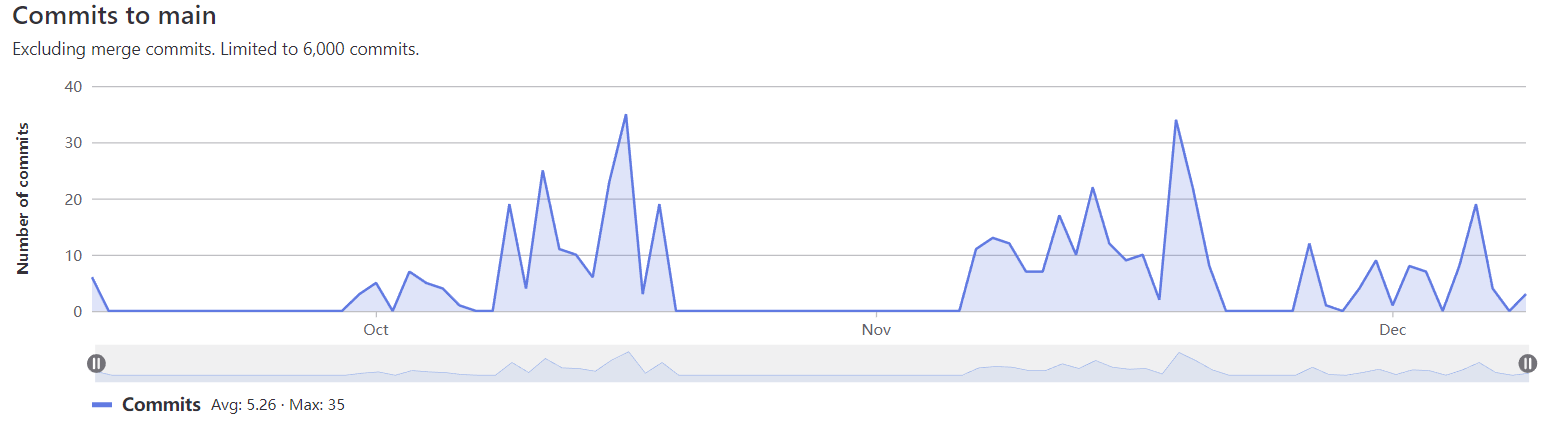
\includegraphics[scale=0.50]{slike/commits_main.png} %veličina
				
				\centering
				\caption{Commitovi na main grani}
				\label{fig:Commitovi na main grani}
				\end{figure}
	
			 \begin{figure}[H]
				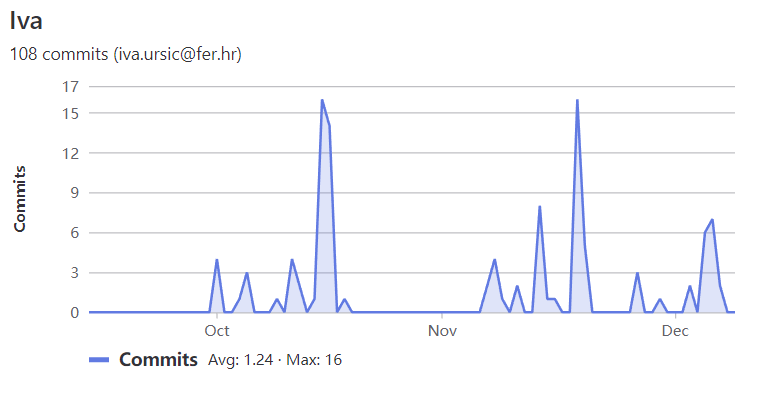
\includegraphics[scale=1]{slike/commits_iva_ursic.png} %veličina
				
				\centering
				\caption{Iva Ursić - commits}
				\label{fig:Iva Ursić commits}
				\end{figure}
			 \begin{figure}[H]
				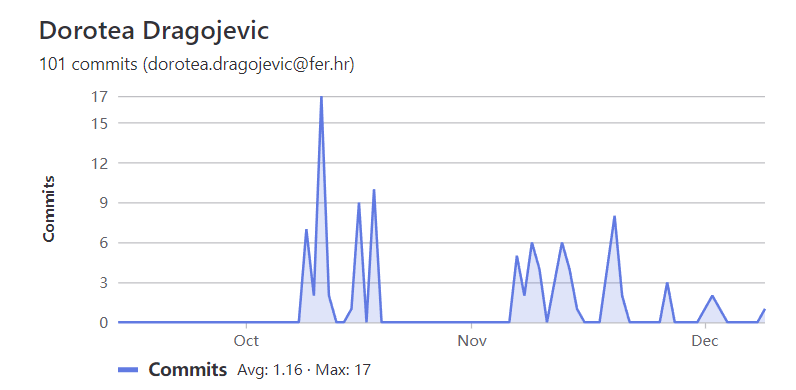
\includegraphics[scale=1]{slike/commits_dorotea_dragojevic.png} %veličina
				
				\centering
				\caption{Dorotea Dragojević - commits}
				\label{fig:Dorotea Dragojević - commits}
				\end{figure}
			 \begin{figure}[H]
				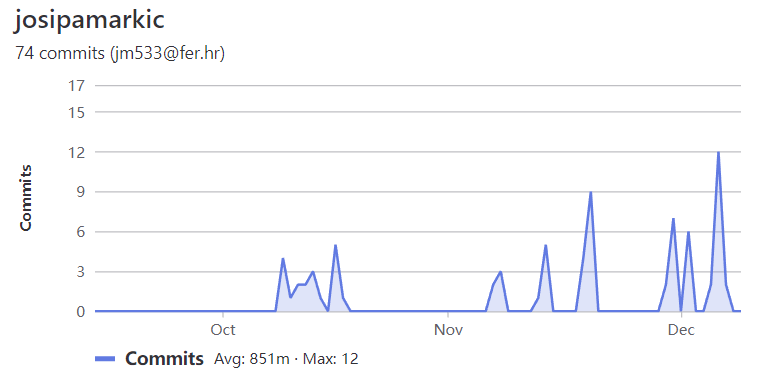
\includegraphics[scale=1]{slike/commits_josipa_markic.png} %veličina
				
				\centering
				\caption{Josipa Markić - commits}
				\label{fig:Josipa Markić commits}
				\end{figure}
		\begin{figure}[H]
				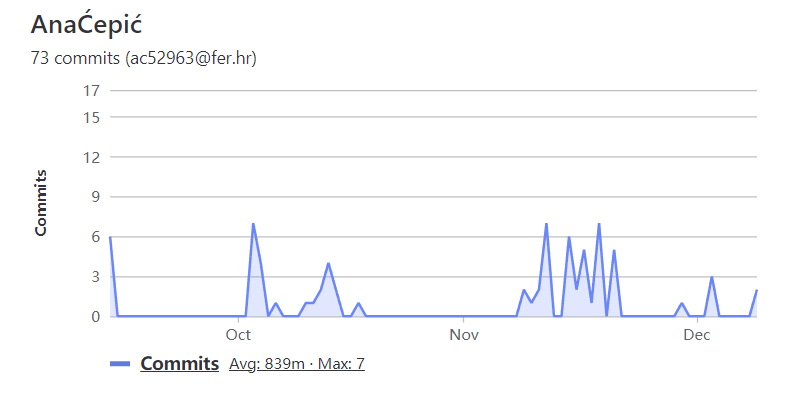
\includegraphics[scale=1]{slike/commits_ana_cepic.png} %veličina
				
				\centering
				\caption{Ana Ćepić - commits}
				\label{fig:Ana Ćepić commits}
				\end{figure}
	
		\begin{figure}[H]
				\includegraphics[scale=1]{slike/commits_nikoleta_benic.png} %veličina
				
				\centering
				\caption{Nikoleta Benić - commits}
				\label{fig:Nikoleta Benić commits}
				\end{figure}
	
		\begin{figure}[H]
				\includegraphics[scale=1]{slike/commits_valentina_valic.png} %veličina
				
				\centering
				\caption{Valentina Valić - commits}
				\label{fig:Valentina Valić commits}
				\end{figure}
	
		\begin{figure}[H]
				\includegraphics[scale=0.50]{slike/commits_andrea_kaselj.png} %veličina
				
				\centering
				\caption{Andrea Kaselj - commits}
				\label{fig:Andrea Kaselj commits}
				\end{figure}
	   
			
		
	
			
		
	


\end{document} %naredbe i tekst nakon ove naredbe ne ulaze u izgrađen dokument 


